%%%%%%%%%%%%%%%%%%%%%%%%%%%%%%%%%%%%%%%%%%%%%%%%%%%%%%%%%%%%%%%%%%%%%%
%%  disstemplate.tex, to be compiled with latex.                    %%
%%  08 April 2002 Version 5                                         %%
%%%%%%%%%%%%%%%%%%%%%%%%%%%%%%%%%%%%%%%%%%%%%%%%%%%%%%%%%%%%%%%%%%%%%%
%%                                                                  %%
%%  Writing a Doctoral Dissertation with LaTeX at                   %%
%%  the University of Texas at Austin                               %%
%%                                                                  %%
%%  (Modify this ``template'' for your own dissertation.)           %%
%%                                                                  %%
%%%%%%%%%%%%%%%%%%%%%%%%%%%%%%%%%%%%%%%%%%%%%%%%%%%%%%%%%%%%%%%%%%%%%%


\documentclass[12pt]{report}    % The documentclass must be ``report''.

\usepackage{utdiss2}            % Dissertation package style file.


%%%%%%%%%%%%%%%%%%%%%%%%%%%%%%%%%%%%%%%%%%%%%%%%%%%%%%%%%%%%%%%%%%%%%%
% Optional packages used for this sample dissertation. If you don't  %
% need a capability in your dissertation, feel free to comment out   %
% the package usage command.                                         %
%%%%%%%%%%%%%%%%%%%%%%%%%%%%%%%%%%%%%%%%%%%%%%%%%%%%%%%%%%%%%%%%%%%%%%

% Some packages to write mathematics.
\usepackage{amsmath,amsthm,amsfonts,amscd} 
\usepackage{eucal}      % Euler fonts
\usepackage{verbatim}   % Allows quoting source with commands.
\usepackage{makeidx}    % Package to make an index.
\usepackage{epsfig}     % Allows inclusion of eps files.
%\usepackage{citesort}  % citesort is ancient and deprecated
\usepackage{cite}   % 
\usepackage{listings}
\usepackage{url}		% Allows nice typesetting of web URLs.
%\usepackage{draftcopy} % Uncomment this line to have the
                        % word, "DRAFT," as a background
                        % "watermark" on all of the pages of
                        % of your draft versions. When ready
                        % to generate your final copy, re-comment
                        % it out with a percent sign to remove
                        % the word draft before you re-run
                        % Makediss for the last time.
% Needed for making certian figures
\usepackage{color}
\usepackage{tikz}
\usepackage{verbatim}
\usetikzlibrary{shapes,arrows}

\author{Anthony Michael Scopatz}    % Required

\address{2906 West Ave. \#16 \\ Austin, Texas 78705}  % Required

\title{Essential Physics Fuel Cycle Modeling \& Analysis}    % Required


%%%%%%%%%%%%%%%%%%%%%%%%%%%%%%%%%%%%%%%%%%%%%%%%%%%%%%%%%%%%%%%%%%%%%%
% NOTICE: The total number of supervisors and other members %%%%%%%%%%
%%%%%%%%%%%%%%% MUST be seven (7) or less! If you put in more, %%%%%%%
%%%%%%%%%%%%%%% they are put on the page after the Committee %%%%%%%%%
%%%%%%%%%%%%%%% Certification of Approved Version page. %%%%%%%%%%%%%%
%%%%%%%%%%%%%%%%%%%%%%%%%%%%%%%%%%%%%%%%%%%%%%%%%%%%%%%%%%%%%%%%%%%%%%

%%%%%%%%%%%%%%%%%%%%%%%%%%%%%%%%%%%%%%%%%%%%%%%%%%%%%%%%%%%%%%%%%%%%%%
%
% Enter names of the supervisor and co-supervisor(s), if any,
% of your dissertation committee. Put one name per line with
% the name in square brackets. The name on the last line, however,
% must be in curly braces.
%
% If you have only one supervisor, the entry below will read:
%
%	\supervisor
%		{Supervisor's Name}
%
% NOTE: Maximum three supervisors. Minimum one supervisor.
% NOTE: The Office of Graduate Studies will accept only two supervisors!
% 
%
\supervisor
    {Erich Schneider}

%%%%%%%%%%%%%%%%%%%%%%%%%%%%%%%%%%%%%%%%%%%%%%%%%%%%%%%%%%%%%%%%%%%%%%
%
% Enter names of the other (non-supervisor) members(s) of your
% dissertation committee. Put one name per line with the name
% in square brackets. The name on the last line, however, must
% be in curly braces.
%
% NOTE: Maximum six other members. Minimum zero other members.
% NOTE: The Office of Graduate Studies may restrict you to a total
%	of six committee members.
%
%
\committeemembers
    [Steven Biegalski]
    [Sheldon Landsberger]
	[Mark Deinert]
	{Man-Sung Yim}

%%%%%%%%%%%%%%%%%%%%%%%%%%%%%%%%%%%%%%%%%%%%%%%%%%%%%%%%%%%%%%%%%%%%%%

\previousdegrees{M.S.E.}
     % The abbreviated form of your previous degree(s).
     % E.g., \previousdegrees{B.S., MBA}.
     %
     % The default value is `B.S., M.S.'

\graduationmonth{August}
     % Graduation month, either May, August, or December, in the form
     % as `\graduationmonth{May}'. Do not abbreviate.
     %
     % The default value (either May, August, or December) is guessed
     % according to the time of running LaTeX.

\graduationyear{2011}
     % Graduation year, in the form as `\graduationyear{2001}'.
     % Use a 4 digit (not a 2 digit) number.
     %
     % The default value is guessed according to the time of 
     % running LaTeX.

\typist{the author}
     % The name(s) of typist(s), put `the author' if you do it yourself.
     % E.g., `\typist{Maryann Hersey and the author}'.
     %
     % The default value is `the author'.


%%%%%%%%%%%%%%%%%%%%%%%%%%%%%%%%%%%%%%%%%%%%%%%%%%%%%%%%%%%%%%%%%%%%%%
% Commands for master's theses and reports.			     %
%%%%%%%%%%%%%%%%%%%%%%%%%%%%%%%%%%%%%%%%%%%%%%%%%%%%%%%%%%%%%%%%%%%%%%
%
% If the degree you're seeking is NOT Doctor of Philosophy, uncomment
% (remove the % in front of) the following two command lines (the ones
% that have the \ as their second character).
%
%\degree{MASTER OF ARTS}
%\degreeabbr{M.A.}

% Uncomment the line below that corresponds to the type of master's
% document you are writing.
%
%\masterreport
%\masterthesis


%%%%%%%%%%%%%%%%%%%%%%%%%%%%%%%%%%%%%%%%%%%%%%%%%%%%%%%%%%%%%%%%%%%%%%
% Some optional commands to change the document's defaults.	     %
%%%%%%%%%%%%%%%%%%%%%%%%%%%%%%%%%%%%%%%%%%%%%%%%%%%%%%%%%%%%%%%%%%%%%%
%
%\singlespacing
%\oneandonehalfspacing

%\singlespacequote
\oneandonehalfspacequote

\topmargin 0.125in  % Adjust this value if the PostScript file output
                    % of your dissertation has incorrect top and 
                    % bottom margins. Print a copy of at least one
                    % full page of your dissertation (not the first
                    % page of a chapter) and measure the top and
                    % bottom margins with a ruler. You must have
                    % a top margin of 1.5" and a bottom margin of
                    % at least 1.25". The page numbers must be at
                    % least 1.00" from the bottom of the page.
                    % If the margins are not correct, adjust this
                    % value accordingly and re-compile and print again.
                    %
                    % The default value is 0.125"

                    % If you want to adjust other margins, they are in the
                    % utdiss2-nn.sty file near the top. If you are using
                    % the shell script Makediss on a Unix/Linux system, make
                    % your changes in the utdiss2-nn.sty file instead of
                    % utdiss2.sty because Makediss will overwrite any changes
                    % made to utdiss2.sty.

%%%%%%%%%%%%%%%%%%%%%%%%%%%%%%%%%%%%%%%%%%%%%%%%%%%%%%%%%%%%%%%%%%%%%%
% Some optional commands to be tested.                               %
%%%%%%%%%%%%%%%%%%%%%%%%%%%%%%%%%%%%%%%%%%%%%%%%%%%%%%%%%%%%%%%%%%%%%%

% If there are 10 or more sections, 10 or more subsections for a section,
% etc., you need to make an adjustment to the Table of Contents with the
% command \longtocentry.
%
%\longtocentry 



%%%%%%%%%%%%%%%%%%%%%%%%%%%%%%%%%%%%%%%%%%%%%%%%%%%%%%%%%%%%%%%%%%%%%%
%	Some math support.                                               %
%%%%%%%%%%%%%%%%%%%%%%%%%%%%%%%%%%%%%%%%%%%%%%%%%%%%%%%%%%%%%%%%%%%%%%
%
%	Theorem environments (these need the amsthm package)
%
%% \theoremstyle{plain} %% This is the default

\newtheorem{thm}{Theorem}[section]
\newtheorem{cor}[thm]{Corollary}
\newtheorem{lem}[thm]{Lemma}
\newtheorem{prop}[thm]{Proposition}
\newtheorem{ax}{Axiom}

\theoremstyle{definition}
\newtheorem{defn}{Definition}[section]

\theoremstyle{remark}
\newtheorem{rem}{Remark}[section]
\newtheorem*{notation}{Notation}

%\numberwithin{equation}{section}


%%%%%%%%%%%%%%%%%%%%%%%%%%%%%%%%%%%%%%%%%%%%%%%%%%%%%%%%%%%%%%%%%%%%%%
%	Macros.							     %
%%%%%%%%%%%%%%%%%%%%%%%%%%%%%%%%%%%%%%%%%%%%%%%%%%%%%%%%%%%%%%%%%%%%%%
%
%	Here some macros that are needed in this document:


\newcommand{\latexe}{{\LaTeX\kern.125em2%
                      \lower.5ex\hbox{$\varepsilon$}}}

\newcommand{\amslatex}{\AmS-\LaTeX{}}

\chardef\bslash=`\\ % \bslash makes a backslash (in tt fonts)
                    %	p. 424, TeXbook

\newcommand{\cn}[1]{\texttt{\bslash #1}}

\makeatletter   % Starts section where @ is considered a letter
                % and thus may be used in commands.
\def\square{\RIfM@\bgroup\else$\bgroup\aftergroup$\fi
  \vcenter{\hrule\hbox{\vrule\@height.6em\kern.6em\vrule}%
                                              \hrule}\egroup}
\makeatother    % Ends sections where @ is considered a letter.
                % Now @ cannot be used in commands.

\makeindex      % Make the index

%
% My Macros
%
%General Short-Cut Commands
\newcommand{\superscript}[1]{\ensuremath{^{\textrm{#1}}}}
\newcommand{\subscript}[1]{\ensuremath{_{\textrm{#1}}}}
\newcommand{\nuc}[2]{\superscript{#2}{#1}}

%%%%%%%%%%%%%%%%%%%%%%%%%%%%%%%%%%%%%%%%%%%%%%%%%%%%%%%%%%%%%%%%%%%%%%
%		The document starts here.                                    %
%%%%%%%%%%%%%%%%%%%%%%%%%%%%%%%%%%%%%%%%%%%%%%%%%%%%%%%%%%%%%%%%%%%%%%

\begin{document}

\copyrightpage  % Produces the copyright page.


%
% NOTE: In a doctoral dissertation, the Committee Certification page
%		(with signatures) is BEFORE the Title page.
%	In a masters thesis or report, the Signature page
%		(with signatures) is AFTER the Title page.
%
%	If you are writing a masters thesis or report, you MUST REVERSE
%	the order of the \commcertpage and \titlepage commands below.
%
\commcertpage   % Produces the Committee Certification
                % of Approved Version page (doctoral)
                % or Signature page (masters).
                %   20 Mar 2002 cwm

\titlepage      % Produces the title page.



%%%%%%%%%%%%%%%%%%%%%%%%%%%%%%%%%%%%%%%%%%%%%%%%%%%%%%%%%%%%%%%%%%%%%%
% Dedication and/or epigraph are optional, but must occur here.      %
%%%%%%%%%%%%%%%%%%%%%%%%%%%%%%%%%%%%%%%%%%%%%%%%%%%%%%%%%%%%%%%%%%%%%%
%
\begin{dedication}
\index{Dedication@\emph{Dedication}}%
For the Horde!
\end{dedication}


\begin{acknowledgments}		% Optional
\index{Acknowledgments@\emph{Acknowledgments}}%
Thank you.  I'll be here til Thursday.
\end{acknowledgments}


% The abstract is required. Note the use of ``utabstract'' instead of
% ``abstract''! This was necessary to fix a page numbering problem.
% The abstract heading is generated automatically.
% Do NOT use \begin{abstract} ... \end{abstract}.
%
\utabstract
\index{Abstract}%
\indent
This document has the form of a ``fake'' doctoral dissertation
in order to provide an example of such, but it is actually a
copy of Miguel Lerma's documentation for the Mathematics
Department Computer Seminar of 25 March 1998 updated in July 2001
and following by Craig McCluskey to meet the March 2001
requirements of the Graduate School.

This document and its source file show to write a Doctoral Dissertation using 
\LaTeX{} and the utdiss2 package. 



\tableofcontents   % Table of Contents will be automatically
                   % generated and placed here.

\listoftables      % List of Tables and List of Figures will be placed
\listoffigures     % here, if applicable.



%%%%%%%%%%%%%%%%%%%%%%%%%%%%%%%%%%%%%%%%%%%%%%%%%%%%%%%%%%%%%%%%%%%%%%
% Actual text starts here.					     %
%%%%%%%%%%%%%%%%%%%%%%%%%%%%%%%%%%%%%%%%%%%%%%%%%%%%%%%%%%%%%%%%%%%%%%
%
% Including external files for each chapter makes this document simpler,
% makes each chapter simpler, and allows for generating test documents
% with as few as zero chapters (by commenting out the include statements).
% This allows quicker processing by the Makediss command file in case you
% are not working on a specific, long and slow to compile chapter. You
% can even change the chapter order by merely interchanging the order
% of the include statements (something I found helpful in my own
% dissertation).
%
%\include{chapter-introduction}

\chapter{One-Group Reactor Methodology}
\index{One-Group Reactor Methodology@\emph{One-Group Reactor Methodology}}
\label{1g_paper}



\section{Introduction}
\index{Introduction@\emph{Introduction}}
\label{1g_sec:intro}
High fidelity coupled neutron transport and fuel burnup calculations require large execution times
and intensive computational resources.  This constraint renders such calculations impractical when 
it is desired to address high level fuel cycle engineering problems on a reasonable time scale.  
The approaches taken in the past to circumvent these time constraints have typically sacrificed 
fidelity by fully decoupling the fuel cycle simulation from physics-based reactor burnup calculations [1].  

Fuel cycle problems revolve around finding the optimum value for a parameter in order to achieve a certain 
global result.  For instance, initial fresh fuel compositions in a reactor may be varied to attain a specific 
burnup. Or repository impact may be of more concern so cooling time before emplacement may be varied.  Even 
the simplest once-through fuel cycle on an isotopic level has a large number of degrees of freedom, each 
featuring a continuum of acceptable values.  Lengthy calculation times for input and output fuel vectors 
in the fuel cycles reactor or reactors make a real parameterization of these degrees of freedom a near 
impossibility.  

Rather than relying on predetermined recipes that limit study to specific cores with precise burnups, 
there is a need for a medium fidelity mechanism that allows for quick, dynamic calculation of burnup 
parameters.  The methodology that is described within details a tool for use in fuel cycle analyses 
that calculates these burnup-related parameters for any arbitrary reactor or interacting fleet of reactors.

The burnup-related parameters include at least the input and output isotopic vectors for the reactor 
as well as the burnup itself, which in turn depends on criticality, allowable fluence, safety issues 
such as reactivity coefficient values, and other constraints.  Other parameters may be of interest 
for specific fuel cycles and will be discussed as they arise.  The burnup tool uses pre-tabulated 
values for the neutron production and destruction rates and the burnup as a function of initial 
isotope present and fluence.  The algorithm then eliminates fluence, giving the burnup only in 
terms of the initial isotopics of the reactor.  The initial isotopics of the core may be iterated 
using this process until the composition that reaches some target burnup is found.  This process 
assumes that there are multiple actinide streams to be blended, and the blending ratios are unknowns 
to be computed.  The output isotopics of the reactor are dependent on initial core composition and 
the burnup, and thus are calculated after other parameters.   This tool may then be embedded within 
a full fuel cycle model.  To demonstrate how such a coupled framework functions, it is applied to 
two fuel cycle concepts.  

The first of the two fuel cycles incorporates a limited uranium recycle strategy.   Uranium from a 
standard pressurized water reactor (PWR) is reprocessed and blended with enriched natural uranium 
(NU) before going into the second core to be burned again.  After this burn, it is noteworthy that 
further recycling via blending is still possible.  In other words, this fuel cycle could be fully 
closed with respect to the uranium stream, avoiding the need to dispose of the reprocessed uranium 
that comprises over 90\% of the mass of spent PWR fuel on an initial heavy metal (IHM) basis.  
This is known as a recyclable uranium (RU) blend and burn fuel cycle since the uranium is reused 
in PWRs, independently of other actinides.  RU blend and burn is an attractive option since it has 
the potential to eventually do a near complete burn of all uranium in LWR spent fuel if used in a 
fully closed cycle.

The second fuel cycle that utilizes the burnup tool developed here demonstrates how the tool may 
be used to improve the fidelity of the fuel cycle material balance calculations associated with 
one of the Global Nuclear Energy Partnership (GNEP) base-case proposals [2].  This case is a 
closed fuel cycle that uses a fast burner reactor (FR) with a conversion ratio of 0.5.  
Actinides are continually recycled in the FR while fission products (FP) are removed and 
disposed.  The reprocessing facility that is built for fast reactor spent fuel has a separation 
efficiency of 0.99 for all actinides.  This is a meaningful option to explore since fast reactors 
are considered to be a key component of long term nuclear energy strategies that close the fuel cycle.

In these two instances the same basic algorithm is used to very quickly solve the blending problem 
to obtain the fresh fuel composition that achieves the desired discharge burnup (BUd); the isotopic 
content of the output is also calculated.   A fuel cycle wrapper governs the mass streams through 
the reactors and other fuel cycle components.  

As will be seen, many fuel cycle parameters may be calculated from the resulting data.  Moreover 
due to the dynamic nature of this method, these parameters will be more accurate and meaningful 
than if a static recipe or simple linearization had been used.  A static recipe would not be able 
to mix recyclable and low enriched uranium (LEU) streams in a way that respects the dependence of 
neutronic characteristics on feed composition, an issue that is inherent to the RU fuel cycle.  
Moreover, models that use static recipes may fail to accurately capture the evolution of material 
balances with each successive pass through a fast reactor.   

The remainder of this paper proceeds via the following layout. The next and second section is a 
full illustration of the burnup model.  The third section is discusses the in depth the recyclable 
uranium and fast reactor fuel cycles to which the burnup model is applied.  The fourth section 
presents the results obtained for these cycles.  The fifth and final section is concludes this 
study and discusses opportunities for future work. 




\section{Burnup Model}
\index{Burnup Model@\emph{Burnup Model}}
\label{1g_sec:bu_model}
The burnup model takes a given input isotopic composition and returns the maximum discharge 
burnup of the fuel as well as its post-irradiation isotopic composition.  Thus, if given a 
target burnup, the model can mix multiple material streams to solve for the fresh fuel composition 
that achieves this burnup.

To form the basis for the burnup model algorithm, certain quantities are assumed to be known.  
The neutron production and destruction rates, the burnup, and the compositional evolution of 
every isotope initially present, namely the actinides and the coolant, are given.  Furthermore, 
they are all specified as functions of fluence (F), the time integral of the total spatially-averaged 
flux in the reactor. A discussion of how to compute and compile these presupposed parameters follows 
later in the burnup model section. 


\subsection{Isotopic Transformation}
\index{Isotopic Transformation@\emph{Isotopic Transformation}}
\label{1g_sec:iso_transform}
The first of the known burnup model parameters is nuclide-specific isotopic transformation as a 
function of fluence, $T_{ij}(F)$ [kg\subscript{j}/kg\subscript{i}].  The subscript $i$ denotes 
the isotope initially present in the core, where as the subscript $j$ labels those nuclides bred in.  
The $T_{ij}(F)$ hence track the transmutation under fluence of the ith isotope into its daughters 
given a nominal reactor spectrum embodied by one-group cross sections.  The daughters tracked 
include both fission products (FP) as well and transuranics (TRU).

\begin{figure}[htbp]
\caption{\nuc{Pu}{239} Transformation as a Function of Fluence for a Sample Fast Reactor}
\label{1g_fig01}
\begin{center}
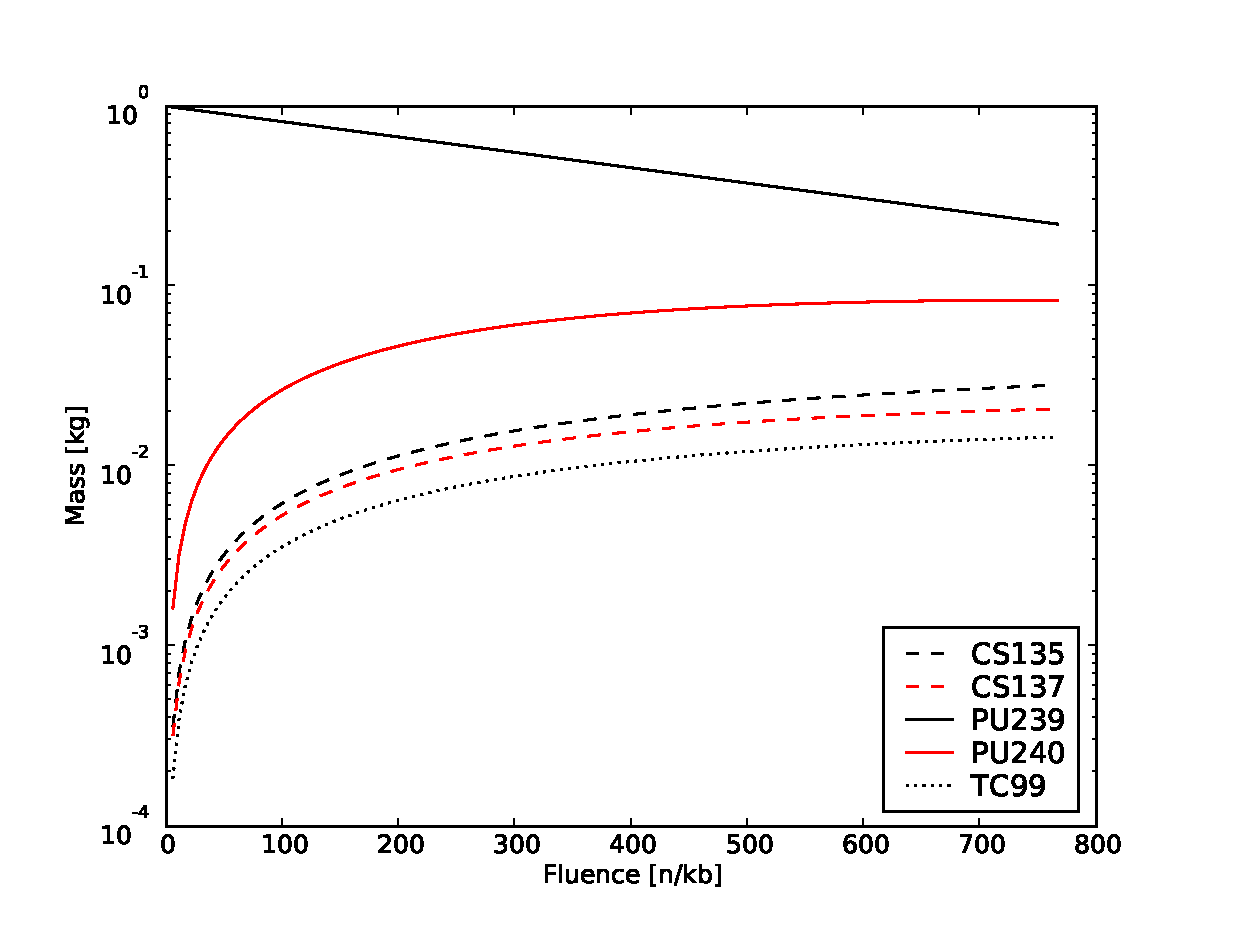
\includegraphics[scale=0.5]{one_group_method/figs/Fig01.eps}
\end{center}
\end{figure}

Figure \ref{1g_fig01} displays an example of this transformation data: the concentration in 
kilograms of tracked isotopes that are present in a sodium-cooled FR core as a function of 1 kg 
of the initial isotope (\nuc{Pu}{239} in this illustration).  In the figure, only one isotope 
(\nuc{Pu}{239} here) is non-zero at zero fluence (ie zero time in the reactor).  For each 
distinct reactor and general fuel type, similar data are required for all other transmuting 
nuclides initially present.   Note that not all species that \nuc{Pu}{239} transforms into are displayed. 

Since this example is for fast reactors, a constant flux of 2×1015 [n/cm2/s] was used when generating the transformation matrices.  For PWRs a constant flux of was 4×1014 [n/cm2/s] assumed.  The units of fluence (F) here are [neutrons/kilobarn], abbreviated [n/kb], while the flux (φ) is again [n/cm2/s], and time (t) is given in [days].

                (1) 

In practice, the Tij data need only exist for the actinides because coolant and structural material transmutation does not significantly impact core neutronic performance  

From here it is simple to apply initial isotopic weight fractions and superposition to Figure 1 and its analogies for all isotopes initially present in the core.  This superimposed result then describes how 1 kg of fresh fuel transforms as a function of fluence within the core. Once the burnup model is applied, the output fluence will also be known, as described below.  Plugging this fluence into the combined data yields the isotopic composition of the fuel at removal. 



\subsection{Neutron Production & Destruction Rates and Burnup}
\index{Neutron Production & Destruction Rates and Burnup@\emph{Neutron Production & Destruction Rates and Burnup}}
\label{1g_sec:pdbu}
Other assumed fuel cycle parameters that are required to perform burnup calculations are the neutron production and destruction rates, pi(F) and di(F) [n/s/flux/kgi].  These are given as functions of fluence for each isotope initially present in the core, just as with the isotopic transformation data.   An example of these parameters is shown in Figure 2.  
(Scopatz, Schneider, Fig. 2)
This figure displays the production and destruction rates for one initial kilogram of 239Pu in the sodium-cooled FR.   
Lastly, the specific burnup for each isotope initially present, BUi(F) [MWd/kgi], is assumed known by the burnup model.  The burnup is defined in the same way as the neutron production and destruction rates.  It is given as a function of fluence for each nuclide initially present in the core.  Figure 3 displays BUi(F) for a few actinides that may be present in the fresh fuel.
(Scopatz, Schneider, Fig. 3)
Now that all quantities assumed to be known have been outlined and defined, a description of the algorithm that calculates the discharge burnup and the input and output fuel isotopics follows.   




\subsection{Solving for BUd and Isotopics}
\index{Solving for BUd and Isotopics@\emph{Solving for BUd and Isotopics}}
\label{1g_sec:solve_BUd_iso}
First, knowing only the BUi(F), pi(F), di(F), and Ti(F) from the prior section, the maximum achievable discharge burnup, BUd [MWd/kgIHM], must be found.  The burnup of the fresh fuel as a function of fluence is then computed as a mass-weighted linear combination of the burnups from the initial constituent isotopes.  Similarly, the neutron production and destruction rates as a function of fluence for an arbitrary fresh fuel may also be found.  In the development below, it is assumed that the core consists of a lattice in which each cell contains two spatial regions, fuel “F” and coolant “C”, but the formulation can generalize to additional regions.  Denote the mass of the ith isotope initially present in the fuel region “F” per unit mass of initial heavy metal (IHM) in the cell by miF [kgi/kgIHM] and the mass of the ith isotope initially present in the coolant region “C” per unit mass of initial heavy metal (IHM) by miC [kgi/kgIHM].  
The volumes of the fuel and coolant regions, VF and VC [cm3], are needed to compute these IHM-normalized masses and the infinite lattice of unit cell model mentioned above is used in modified form for this purpose.  This two region method ignores the small effect of the cladding material on neutron capture.  Call r [cm] the radius of the fuel pin and l [cm] the pitch of the unit fuel cell.  It is important to correct for the fact that not all fuel pin slots in a fuel assembly are filled with fuel.  Denote ST as the total number of pin slots in a fuel assembly and SO as the open, non-fuel containing slots.  The effective volumes are then given in Equations 2 & 3.
                                         (2)
                         (3)
Hence the burnup of the core as a function of fluence, BU(F) [MWd/kgIHM], is given by the following sum.
                                (4)
Once this burnup is known, the maximum discharge burnup can be computed as that value of burnup for which the core ceases to be critical.  The fluence-dependent neutron production and destruction rates for each constituent are used here to compute the multiplication factor, k.    When k drops below unity, a reactor full of this fuel will no longer be able to sustain a chain reaction.  k(F) is approximated by calculating the full-core neutron production rate, P(F) [n/s/kgIHM], divided by the full-core average neutron destruction rate, D(F) [n/s/kgIHM].  Namely,
                                                  (5)
k(F) may thus also be calculated, like BU(F), as a mass-weighted convolution of the pi(F) and di(F).  The method by which one obtains P(F) and D(F) from the isotope-specific rates is discussed in the following sections.  However once known, k(F) is then set equal to one and then Equation 5 solved for the fluence.  This is the fluence at discharge and is called Fd [n/kb].  Fd may then be reinserted into Equation 4 and the burnup of the fuel composition at discharge, BUd [MWd/kgIHM], is attained.
Note that Equation 5 can hold for a multi-batch fuel management scheme as well as a one batch core system.  Extending this equation to a multi-batch system follows after a discussion of the calculation of P(F) and D(F).
Additional factors complicate the calculation of the core-average neutron production and destruction rates.  A complete depiction of the neutron balance requires that pi(F) and di(F) for non-fuel components of the core must also be known.  These non-fuel components include the coolant outside of fuel regions and the non-actinide species in the fuel region (e.g. oxygen in UOX).  Both of these classes of parasitic species serve to increase the full core destruction rate.  Disadvantage factors also affect the flux suppression in fuel regions which needs to be accounted for as well for PWR cases.  Furthermore, to account for spatial variation in the neutron flux when computing neutron interaction rates in non-fuel components, a general fuel assembly model is needed (as described above).  For example, to reflect a standard PWR fuel assembly geometry values from the OECD Burnup Credit Criticality Benchmark [3] were used for LWRs and nominal values for fast reactors were taken from [4].  A walkthrough of how to calculate the core-average production and destruction rates, P(F) and D(F), from the known set of pi(F) and di(F) for a given collection of mi now follows.  



\subsubsection{The Neutron Production Rate}
\index{The Neutron Production Rate@\emph{The Neutron Production Rate}}
\label{1g_sec:p_rate}
 The pi(F) and di(F) are superimposed to build the full-core loading.  These rates reflect the evolution of the neutron balance for an initial unit mass of the species i when exposed to the neutron flux spectrum extant in the reactor being studied.  Therefore they are computed using cross sections prepared for a specific reactor and fresh fuel composition.
However as mentioned above, flux spectra and magnitudes are spatially dependent.  The most basic geometric model and the one again used is that of an infinite lattice of unit cells consisting of a central fuel region surrounded by a coolant-filled region.  These two regions have neutron production and destruction rates that are distinct since the set of mi that are used in each region is different.  Once again, use the superscript “F” to denote a parameter relating to the fuel region and the superscript “C” for the coolant region. 
The production rates for the fuel and coolant regions, pF(F) and pC(F) [n/s/flux/kgIHM], can be calculated in direct analogy to Equation 4 for the burnup.  The neutron production rate in the fuel region is 
                                (6)
and pC(F) = 0 since the coolant contains no neutron producing isotopes.  
The advantage of this algorithm is easily seen through Equation 6.  By assuming that isotopic production and destruction rates are known, superposition is then used combine the individual rates into full-core or region specific rates.  This allows for fast recombining of core constituents without having to recalculate the isotopic rates from scratch.  For instance, to calculate the burnups achievable from 2% and 4% 235U enriched PWR fuel would typically require distinct computationally intensive runs because of differing initial fuel compositions.  With this method all that is needed is to change the mi used in Equation 6 and also perhaps to obtain case-specific burnup parameters pi(F), di(F) and BUi(F) by interpolating between a handful of precomputed sets.  
However, the fuel region production rate is not equivalent to the full-core production rate.  There is one core effect that is not seen at the fuel cell level: leakage.  To capture this macroscopic effect a non-leakage probability PNL is introduced.  The PNL effectively reduces the production rate of neutrons for the core. The PNL used is characteristic of the reactor design and composition; it may be computed using macroscopic transport methods, but in practice it is used as a calibration parameter.  Finally then, the full-core production rate is given simply as 
                                        (7)
Note that P(F) here is normalized to a unit mass of IHM.  Thus P(F) has units of [n/s/kgIHM], and the neutron destruction rate will be normalized in the same way.



\subsubsection{The Destruction Rate}
\index{The Destruction Rate@\emph{The Destruction Rate}}
\label{1g_sec:d_rate}
The full-core destruction rate, D(F), is calculated in the same manner as the fuel region production rate.  However, the other nuclides in the reactor, while not contributing to fission, do contribute to neutron destruction in the core. Similarly, the burnup BUi(F) for these nuclides will also be zero since fission does not occur. In fuel cell model used above, two other isotopes are present in a PWR core (16O and 1H) and one other main species in a FR core (23Na).
The following example walks through the calculation of D(F).  First, start with the fuel region destruction rate dF(F) in analogy to the fuel region production rate Equation 6.  Note that the units of dF(F) are [n/s/flux/kgIHM].  
                                (8)
Moreover, the coolant can strongly contribute to the destruction rate.  However, it is important to take into account that for some fuel/coolant combinations the flux is not spatially uniform; for instance in PWRs the thermal flux is generally higher in the coolant than in the fuel. To account for this, a disadvantage factor is introduced.  For other reactor types, for example FRs, the flux profile is much flatter over the unit cell and a disadvantage factor is not necessary. The disadvantage factor ζ is qualitatively the average flux in the moderator divided by the average flux in the fuel. The fuel suppresses the thermal flux levels so ζ will always be greater than one and the flux in the moderator will always be greater than the flux in the fuel. Since it is dependent on the composition of the fuel, ζ is therefore also a function of the fluence because the fuel isotopic makeup is altered as a function of fluence. A fuller look at how to calculate ζ(F) can be found in [5].  Figure 4 shows how ζ(F) changes with fluence for two LEU fuels with 3.2% and 4.3% 235U. 
(Scopatz, Schneider, Fig. 4)
Thus the coolant destruction rate is then given as
                        (9)
Note that the volumetric weight in miC for the coolant region already includes both empty and filled fuel pin slots.  Therefore the full-core destruction rate D(F) is given by the sum of the destruction rate in the fuel and the destruction rate in the coolant.  Namely, 
                                (10)
Now that P(F) and D(F) are known, k(F) may be calculated as per Equation 5.  Once again, Fd is defined such that k(Fd) = 1 which yields the maximum discharge burnup BU(Fd) = BUd.



\subsubsection{Multiple Batch Cores}
\index{Multiple Batch Cores@\emph{Multiple Batch Cores}}
\label{1g_sec:batch_ave}
What has just been shown is how to find the discharge burnup with a given fuel composition for a one batch system.  However, for multiple batches of fuel the process is less straightforward as the production and destruction rates are averaged over their end of cycle values for each batch.  The general idea is to perform these operations in reverse and then iterate over them.  In other words, one picks a burnup and then solves for the multiplication factor.  Then one picks another burnup that will yield a k closer to one and solves again for k.  This process continues until a k is found that is acceptably close to one.  
The bisection method is preferred to pick successively closer values of k.  It is not prone to the erratic behavior that arises when Newton’s method is used with pointwise data.   Furthermore, the bisection method ensures that the fuel is burnable.  To use the bisection method here there must be both some fluence where k < 1 and some fluence where 1 < k.  Since the multiplication factor is in reality continuous and more or less monotonic, these conditions imply that at some fluence k = 1.  However, if these conditions fail then the fuel has too little fissile material to sustain a chain reaction. 
(Scopatz, Schneider, Fig. 5) 
(Scopatz, Schneider, Fig. 6)
A walkthrough of the details of this process for multiple batches follows.  First, a maximum discharge burnup BUd is guessed.  Say without loss of generality that the system at hand is concerned with a three batch refueling cycle.  Then, assuming equal interbatch power sharing, the fluence must be found for three burnups, namely BUd, 2/3 BUd, and 1/3 BUd.   Lines drawn on Figure 5 from the burnup axis to the curve and then down from the curve to the fluence axis will give the fluence at the three points required.  Note that the highest fluence (F3 here) is the fluence at discharge Fd.  After the fluence for each of the burnups has been calculated, the multiplication factor of the system needs to be known. 
To achieve this for a multibatch core, a flux-weighted batch averaging procedure is followed.  The multiplication factor at each fluence is determined by the P(F)/D(F) ratio.  Denote the batch number that a parameter is associated with by the index subscript “b”.  In Figure 6, the three kbs correspond to the three fluences chosen and here kb(Fb) = Pb(Fb)/Db(Fb).  These are interpreted as the multiplication factors if the full core was in fact composed entirely of fuel that had been exposed to this fluence. Thus the true multiplication factor of the core is the weighted average of the production divided by destruction rates with the flux as a weight for “B” number of batches.
                                                (11)
However, the flux φbin Equation 11, the average flux within batch b, is not known.  Thus because the batch power remains constant φb does not.  Yet the flux is by definition the time derivative of the fluence. Thus a good approximation of the flux is given in Equation 11.
                                                (12)
Here, ∆F can be measured at a given fluence by perturbing BU(F) by a small amount and finding the ∆BU.  This is easily done as ∆BU / ∆F is identically the slope of the BU(F) graph at fluence F as seen in Figure 5.  Given the assumption of constant power density, a change in burnup yields a corresponding change in time such that
                                        (13)
Where BUd is the discharge burnup guess and Tres [days] is the residence time that the fuel took to achieve this discharge burnup. Combining Equations 12 and 13, φb is found to be
                                        (14)
Inserting Equation 14 into Equation 11 an expression for the effective multiplication factor for a multiple batch system at the time that a batch is discharged is obtained.
                        (15)
Now that a k has been found, its value is converged to unity via the bisection iterations.  Another value of the maximum discharge burnup is then chosen and this process is repeated until a BUd is found that yields a k = 1.  Figures 5 and 6 represent the process of finding a multiplication factor for a sample three batch system for a fast reactor core.  
In the process of determining the maximum discharge burnup Fd is also found.  It is also easy to perform a mass-weighted linear combination of the isotopic transformation matrices. From here how each isotope initially present is transmuted at any fluence is known.  The mass of the jth nuclide at fluence F is called Mj(F) [kgj/kgIHM] and is given by

                                 (16)
Here “i” represents isotopes initially present in the fuel.  Plugging in the fluence at discharge Fd into Equation 16 will yield the mass of isotope “j” in the spent fuel per kilogram of IHM.  Performing this operation for all “j” isotopes of interest will yield the isotopic output vector for the core.  Since fission product masses were included in the transformation matrices, the fission products at discharge are also known.  
(Scopatz, Schneider, Fig. 7)
Figure 7 shows a graphical representation of the Mj(F) for various isotopes present in a fast reactor.  Each curve for each nuclide is the superposition of all of the transformation matrices with their weight, as described above.  Some species, such as 238U and 239Pu, are burned out of the core faster than they are bred back in and are therefore represented by lines of negative slope.  Other isotopes, namely fission products, were not initially present and get bred into the core by any fissioning species.  These are shown as the curves growing towards some asymptote.  Still other nuclides, higher order species like 243Am and 244Cm, have a more dynamic effect.  They grow into the core and then peak and start to burn out.  
In conclusion, the above is an algorithm for finding the maximum discharge burnup and its discharge composition given only a fuel form represented by mi, the pre-generated burnup parameters (pi(F), di(F), BUi(F), and Tij(F)), the number of batches in the core B, and the non-leakage probability PNL.  However, methods for generating these burnup parameters have not been discussed.  This follows in the next section. 



\subsection{Generating Burnup Parameters}
\index{Generating Burnup Parameters@\emph{Generating Burnup Parameters}}
\label{1g_sec:gen_BU_param}
The burnup parameters pi(F), di(F), BUi(F), and Tij(F) are typically calculated for a specific reactor design.  However, if the reactor type is perceived as being representative of all reactors of that type then the burnup parameters may be applied generally to all reactors of this type without having to recalculate new pi(F), di(F), BUi(F), and Tij(F).  Qualitatively, what it means to be representative of a reactor type and fuel composition is that the neutron energy spectrum inherent in the few-group cross sections used to generate the burnup parameters is similar to that of other reactors of this type and other fuel compositions that will be studied.   
In this study, the burnup parameters are calculated and tabulated based on the reactor-specific data libraries created from ORIGEN 2.2 [7] isotope-by-isotope burnup analyses.  As mentioned, the ORIGEN input libraries contain cross sections that are thought of as generic to a reactor type and range of fuel compositions.  For example, the libraries used here for fast reactors were prepared for a sodium cooled burner reactor with a target conversion ratio of 0.5.  This reactor is described in more detail in [4].  The burnup model therefore utilizes pre-computed libraries of the pi(F), di(F), BUi(F), and Tij(F) that were built up from ORIGEN runs.  These libraries contain point wise data as a function of fluence.  Recall that all data in these libraries track the evolution of the parameter on a per unit mass basis.
To be more explicit, ORIGEN 2.2 is run for a kilogram mass of a given nuclide with the characteristic ORIGEN libraries.  Therefore, the isotopic mass balances and reaction rates obtained from this run reflect the evolution of one kilogram of this isotope within the core.  The ORIGEN output is then parsed and placed in the appropriate libraries for usage by the burnup model.  These ORIGEN runs are performed for all nuclides in the core.  Naturally, if one were to use initial ORIGEN libraries for a different reactor type, then the tables and matrices generated here would be representative of this other reactor.  These libraries only need to be generated once ever for a given reactor type, geometry and representative fuel composition.
In addition, the representative cycle-average neutron energy spectrum changes with BUd.  This is because more fissile fuel is needed to achieve increased burnups and even for an identical fuel to coolant volume ratio the spectral dependence on burnup is often too large to neglect.  Thus for thermal-spectrum systems ORIGEN input libraries are prepared for a number of differing BUds: for PWRs, for instance, libraries representative of 20, 33 and 50 MWd/kgIHM discharge burnups have been used in these studies.  Thes libraries are interpolated to create customized libraries at any burnup in this range.  They thus capture the dependence of the cycle-average cross sections on discharge fluence and, implicitly, initial isotopics.  This is of more significance to PWRs as fast reactor spectra are relatively more stable; moreover, to investigate high-burnup PWR fuels additional libraries for BUd of 70 and 100 MWd/kgIHM have been prepared using assumed initial 235U enrichments of 5.5 and 8 w/o, respectively..
Even systems whose spectra are less sensitive to initial composition and burnup must be treated using a number of cross section libraries prepared from detailed transport calculations.  For the sodium-cooled FR design studied here, for example, a number of libraries are available.  The core aspect ratio for the design varies to ensure acceptable coolant void reactivity properties as the conversion ratio and uranium content decrease, so distinct sets of libraries were prepared for 0.5 (used in this study) and 0.25 target conversion ratio designs.  Additionally, separate libraries were prepared at each conversion ratio for fuels with higher and lower minor actinide (MA) content.   The higher MA case is representative of the feed to a FR if Pu from spent UOX is first burned in MOX, while the lower MA library, the one used in this study, reflects the TRU content with no MOX burn.



\subsubsection{Hydrogen Cross Section Rescaling}
\index{Hydrogen Cross Section Rescaling@\emph{Hydrogen Cross Section Rescaling}}
\label{1g_sec:H_rescale}
The one group cross sections are functions of fuel burnup and therefore fluence, in some cases quite strongly so.  The model supports the adjustment of cross sections – and therefore production and destruction rates as well as transmutation rates – with fluence.  For instance, the effective one group radiative capture cross section of 1H in typical PWR coolant changes significantly with fluence as the flux spectrum in the core evolves to maintain constant power density.  Just as with the interpolation of the ORIGEN input libraries, the hydrogen cross section may be parameterized around the burnup that the core has experienced.  Moreover, hydrogen contributes about 10% to the total destruction rate in the core.  Thus a significant change in the hydrogen cross section could yield an appreciable error in the model as formulated above.  What follows is more of an adjustment to the hydrogen one-group cross section than a true mutli-group theory response.  However, this provides an easy to calculate and integrate model to reduce the error induced into the neutron destruction rates.
To account for these spectral variations an f-factor is introduced that is a function of the burnup BU(F).    f(F) is a unitless factor by which all hydrogen destruction rates dH(F) are multiplied by in Equations 8-10. Two hydrogen cross sections are known for two burnups.  These were taken from the ORIGEN cross section libraries prepared for 33 and 50 MWd/kgIHM burnups in PWRs.
f(F) is the computed by drawing the line between these two points and dividing it by the cross section that was used for the ORIGEN runs.  Since ORIGEN was run using the 33 MWd/kgIHM library, the line is simply divided by 0.03474 barns.  The equation for f(F) is therefore, 
                        (17)
As is seen in this extrapolation, the per atom hydrogen neutron destruction rate can vary considerably.  Multiplying f(F) by dH(F) results in an increase of the accuracy of all destruction rate and multiplication factor data that is computed.  The inclusion of the hydrogen rescaling factor and subsequent effects on BUd and initial compositions will be discussed in a later section with regards to the example of standard PWRs.  



\section{}
\index{@\emph{}}
\label{1g_sec:}
3 Fuel Cycles:
The Global Nuclear Energy Partnership (GNEP) plan for domestic fuel cycles offers many possible pathways.  With most of these options GNEP hopes to reduce the stockpile of United States transuranics (TRU) and obviate the technical need for a second repository during this century.  Separated transuranics are moreover seen as dangerous to nuclear non-proliferation goals.  Furthermore, most TRU species negatively impact repository performance as compared to an equivalent mass of NU.  Two fuel cycles involving recycle – uranium recycle in PWRs and full TRU recycle in FRs – are examined here as case studies to which the method presented above is applied. 


\subsection{Uranium Recycle Fuel Cycle}
\index{Uranium Recycle Fuel Cycle@\emph{Uranium Recycle Fuel Cycle}}
\label{1g_sec:UFC}
The first of the fuel cycles that are analyzed here explores blending of RU with enriched NU to achieve sustained uranium recycle in light water reactors (LWR).  Since RU is a product of reprocessing of light water reactor spent nuclear fuel (LWR SNF), the front end for the RU creation process includes the back end of the reprocessing based LWR-NU fuel cycle.  The application of the burnup model to the RU burning reactor will be demonstrated through the study of this fuel cycle.
Figure 8 depicts the RU blending option studied here.  Red arrows in Figure 8 connote RU flow stemming from the UREX+ reprocessing component or the enrichment component.  Black arrows that lead out of components indicate flows that do not comprise the mass input streams to the RU burning reactor.  
(Scopatz, Schneider, Fig. 8)
Blending RU with enriched natural uranium is a method of increasing the fissile content of the RU while also impeding the buildup of 236U, a neutron poison.  From the standpoint of the fuel cycle material balance alone, if the utilization of RU is to be maximized the best material to serve as a blend stock with RU is highly enriched uranium (HEU).  HEU is in limited supply as a blend stock [8] and its use for civilian applications is undesirable; therefore, if this strategy is to be sustained, the blend stock would be low enriched uranium (LEU).  
LWR SNF contains a higher enrichment of 235U than NU; therefore RU blending may be economically advantageous over the once-through fuel cycle given that reprocessing is already taking place to recover TRU. The weight percent of 235U in the legacy spent fuel of the United States is between 0.8-0.9% [6].  However, LWR SNF also has had 236U bred into it in non-negligible amounts of around 0.3-0.5%.  As 236U is a neutron poison, the advantage of the extra 235U in RU is not immediately quantitatively obvious.  Therefore, to increase the fissile content of an RU fuel form, it is blended with LEU. This LEU blend stock serves to dilute the 236U and thereby decrease its negative impact on the neutron balance in the core. 
Fuel that goes into the RU reactor must be assigned a target burnup; for reasons of simplicity and practicality, it will be assumed that it is desirable to achieve parity between the traditional LEU- and RU-bearing fuel burnups.  Since the RU isotopic composition is set by the burnup in the initial reactor, the free parameters that are used to match the burnup of RU fuel to that of virgin LEU fuel in the reactor are the LEU enrichment and its mass fraction in the blended LEU-RU stream.    
The first blending option is that the mass of LEU blend stock per unit mass of RU is held constant.  Thus the fissile content of the RU-bearing fuel is controlled by the enrichment of the LEU.  On the other hand, the LEU enrichment can be held constant and the mass that is mixed with the RU may be varied.  In this second case the LEU enrichment may be up to 19.9%.  
It should be noted that higher LEU enrichment levels mean that more RU can be blended for a given mass of LEU.  But generally, near-future enrichment plants will not be licensed to produce LEU at greater than 8% 235U enrichment. However, the LEU/HEU limit is 19.9% so it is conceivable that if RU recycle came to fruition civilian enrichment facilities would be allowed to produce 19.9% enriched product.  



\subsection{Fast Burner Reactor Fuel Cycle}
\index{Fast Burner Reactor Fuel Cycle@\emph{Fast Burner Reactor Fuel Cycle}}
\label{1g_sec:}
A fuel cycle that features full, sustained TRU recycle is the second one being examined.  The basis of the model used here is a fast reactor (FR) with LWR SNF top up.  The purpose of this fuel cycle option is to reduce the global actinide inventory per unit energy as compared to the standard once-through fuel cycle, with the specific aim of reducing transuranics.   To this end, the FR conversion ratio (CR) is less than unity.  The nominal value for the conversion ratio in this study is taken to be 0.5, consistent with the baseline sodium-cooled fast transmuting reactor point design used in GNEP scoping studies [2].  
(Scopatz, Schneider, Fig. 9)
Figure 9 depicts the FR fuel cycle that is being studied.  Once again, mass flows represented in red are the four mass streams that form the FR fresh fuel blend stock.  The mass of each stream relative to the others may be varied by the burnup model to achieve a target burnup.  The mass flows in black are the flows that are considered static to the burnup model and are not changed, though they may vary with fuel cycle pass number.  
Moreover because of the dynamic nature of the burnup model, the discharge burnup is not fixed but rather a target BUd is set as a parameter within the model.  Alteration of the BUd will change the balance of the FR input mass streams as well as all dependent isotopics.  However, burnup values of 51 MWd/kg for the LWR and 170 MWd/kg for the FR are used unless otherwise stated.  Both of these values were taken from the VISION [1] specifications for nominal LWR and FR cases.  Similarly, spent fuel from both the LWRs and FRs is allowed to cool for a time before being reprocessed.  The time that spent fuel of any sort is allowed to cool also affects the isotopics and mass stream material balances.  But once again, the cooling time is a parameter that may be specified within the fuel cycle model for which nominal values were taken here.
The input mass to the fast reactor is made up of four independent streams: the uranium coming from light water reactors (LWR-U), the transuranics coming from light water reactors (LWR-TRU), the uranium coming from fast reactors (FR-U), the transuranics coming from fast reactors (FR-TRU).  These streams are separated in the reprocessing facilities and then combined to form the input stream to the fast reactor.  The fission products from these streams are also removed from the fuel at this point and sent off to a disposal facility.  
It should be noted here that the reprocessing facility that deals with the light water reactor spent nuclear fuel (LWR SNF) and the reprocessing facility that handles the fast reactor spent nuclear fuel (FR SNF) are not the same.  They are displayed as one box in fuel cycle Figure 8 for ease of reading, although it is likely that these two fuel cycle components would be collocated.
Lastly, Figure 9 represents a closed fuel cycle which implies that actinides may be recycled indefinitely or until they are eventually burned as long as there exist enough FRs to handle the mass throughput.  Of course this is not strictly true since no separation process is perfect.  Some small actinide mass will be mixed with the fission products after reprocessing and be sent to the repository.  It is known that the reprocessing separation efficiencies ultimately affect repository performance [11].  However, because the isotopics change with every pass of TRU through the fuel cycle, there arises a mass stream feedback between the reactor burnup, the cooling time, and the reprocessing efficiencies that the burnup model handles with ease. 
The implication of a closed or partially closed fuel cycle is that mass may be sent through many recycles.  For a specific target FR burnup and other fuel cycle parameters, the relative masses and the isotopics of the four mass streams (LWR-U, LWR-TRU, FR-U, FR-TRU) may change significantly as a function of pass number.  However, one would eventually expect that equilibrium values for the mass balances and isotopics will be reached and indeed they typically are.  For some species, though, so-called equilibrium is not reached even after many recycles; indeed, in practice many decades, even centuries, would elapse before an ‘equilibrium’ scenario result would reflect reality.  Therefore, equilibrium fuel cycle simulation results must be interpreted with caution.  When equilibrium is achieved and how it is defined is discussed further in a later section.  



\subsection{Cooling Model}
\index{Cooling Model@\emph{Cooling Model}}
\label{1g_sec:cool_model}
Before reprocessing occurs, light water reactor spent nuclear fuel (LWR SNF) and fast reactor spent nuclear fuel (FR SNF) are typically stored and cooled.  This process represents the “Storage” boxes in fuel cycle Figures 8 and 9.  The cooling model computes the analytical solutions to the Bateman equations [12]: 
        (18)
Here, tC [years] is the time that the SNF spends in storage cooling,  Ni(tC) [kg] is the mass of the ith daughter of the parent species with mass N1 [kg]. The λs [1/years] are the decay constants for the respective nuclides in the decay chain.   The γs are the branch ratios that correspond to each decay constant for this decay chain.  
Finally, these results are sent to the reprocessing model (where separation efficiencies are applied), output parameters are recorded, graphs are generated, and (for the FR case) the next cycle starts.   It is therefore time for the dynamic fuel cycle results to be computed using the burnup model.





\section{The Fuel Cycle Model: Benchmarking & Results}
\index{The Fuel Cycle Model: Benchmarking & Results@\emph{The Fuel Cycle Model: Benchmarking & Results}}
\label{1g_sec:fcmodel_benchmark}
The fuel cycle model is the computational wrapper that executes much of the calculation and analysis.  The fuel cycles that are studied are specified by a large set of inputs extending to the various intrinsic parameters of the reactors that comprise it.  For example, the PNL of the different reactors are specific to that reactor’s design and neutron transport characteristics.  Other parameters include the reactor’s target burnup, the amount of time that SNF spends in storage cooling, and the fuel cell specifications that are used.  Values for these parameters that were used in this study are presented in Table 1.  Knowing this information, the fuel cycle model wraps around the reactor burnup model and invokes it when input streams need to be mixed or spent fuel compositions must be found.  The fuel cycle model then sends the results of the burnup model to the next fuel cycle component (as seen in Figures 8 and 9).  Thus the fuel cycle model coupled with the burnup model developed here to produce unique, physics-based values for the material balances and isotopics for one or many recycle passes.  This represents an advantage over recipe based simulations which are not able to alter any of the input parameters at will whereas here all of them are allowed to change. 
(Scopatz, Schneider, Table 1)
It is important to point out that the burnup model is sensitive to the input parameters specified in Table 1.  To select the non-leakage probability PNL and calibrate the model, enrichment and burnup combinations were taken from VISION [1] libraries for LEU for a 3 batch core.  By thinly varying PNL and the coolant density ρC [g/cm3] and toggling the f-factor correlating cycle-average hydrogen cross sections with discharge burnup a wide range of values for enrichment for given burnups was generated.  These are presented in Table 2 along with benchmark enrichment/burnup values taken from two other sources.  The parameter set H was the one that was chosen for the actual model as it most closely represents reality and the VISION targets.  Note that the enrichment is in weight percent 235U and BUd is in units of [MWd/kgIHM].  This calibration must be carried out for each reactor system to be analyzed.
(Scopatz, Schneider, Table 2)
A series of benchmarks were carried out to verify both the fresh fuel composition and fuel burnup calculations.  The OECD Burnup Credit Criticality Benchmark [3] series is a composite of many international studies using independent, high fidelity neutronics codes acting on the same specifications.  The study selected for benchmarking, Phase I for PWRs, uses an initial fuel vector (3.6 w/o 235U with trace amounts of 234U and 236U) that is burned to 40 MWd/kg.  The study lists output isotopics at various stages during the burn and post-removal cooling.  
To benchmark the burnup algorithm developed here, the initial fuel vector and burn parameters are taken from the study but “generic” PWR cross section sets were used.  In other words, the cross sections developed for a reference 17x17 PWR lattice were used with the burnup model and detailed transport calculations to create customized cross section sets for the benchmark case were not carried out.  This situation reflects the procedure that might actually be carried in a fuel cycle scoping calculation, where it is desirable to treat all reactors of a single general type as represented by a generic archetype.  Table 3 compares the computed isotopics to the isotopic vector reported in the OECD study for a 40 MWd/kgIHM burn with no cooling.  The table also shows the standard deviation of the collected results for the 21 participants in the Phase-IB study.  
(Scopatz, Schneider, Table 3)
All values are given in terms of weight percent of initial heavy metal.    These results show that the present method matches the Burnup Credit within two standard deviations for most actinides.  The only species showing a much larger relative departure is 241Am.  241Am is formed almost exclusively thorugh 241Pu decay and there are two reasons for this departure.  First, the fluence-dependent isotopic transformation matrices were assembled using a constant flux 4x1014 [n/cm2/s] that is representative of most PWRs.  If the average flux and power density are somewhat lower, and hence the irradiation time is somewhat longer as is the case here, the model will under predict the 241Am buildup in the core.   Second, the model does not explicitly treat refueling downtimes when transmutation ceases but decay continues. Note that the deviation in long-term 241Am content is smaller because the concentration of the much more abundant parent, 241Pu, is reasonably accurate. 
It is also necessary to benchmark the feed stream blending and discharge burnup calculations.  This is best achieved in the context of a comparison of a fuel cycle material balance.  Material balances of this type generated using the high-fidelity material balance simulation package COSI [14] are available in a number of OECD systems studies, e.g. [15].  A benchmark of the equilibrium material balance for a PWR/FR fleet has been carried out.  In this benchmark, the methodology described here is used to find the enrichment of PWR fuel to achieve a specified burnup as well as to derive the equilibrium FR fresh and spent fuel compositions through the cycle iteration procedure described in this paper.  Specific results benchmarked included the PWR/FR thermal power split, the isotopic composition of the burned fuel, and the fuel cycle cost derived from the material balance flowsheets.  A detailed description of the benchmark results may be found in section 3.2 of the companion paper [13] appearing in this issue.  Since the benchmark fuel cycle scenario served as a point of departure for the system study presented in that paper, and also because items outside the scope of this paper such as cost calculations were being benchmarked, it was felt more appropriate that this benchmark be presented there.





\subsection{The Recyclable Uranium Fuel Cycle}
\index{The Recyclable Uranium Fuel Cycle@\emph{The Recyclable Uranium Fuel Cycle}}
\label{1g_sec:RUFC}
The RU fuel cycle described here does not preclude multi-recycle of transuranics; instead it focuses only upon the uranium component of an integrated recycle strategy.  Moreover, for purposes of illustration only the first uranium recycle pass is considered.  A second example applying the burnup model to a dynamic case will be covered in the FR fuel cycle section.
To further characterize what is happening in the burnup model, it is of interest to characterize the isotopic breakdown of the neutron production and destruction rates in the core.  To do so, one simple case is considered.
For this illustrative case the 235U enrichment is chosen at 4.0%, while the 236U enrichment is set to 1.5%.  Three batch fuel management is assumed and a graph of BU(F) is made in analogy to Figure 5.  The discharge burnup BUd of this fuel is not known a priori but it is instead calculated via the burnup model that was described above.  BUd here turns out to be approximately 37 MWd/kgIHM.  Figures 10, 11, 12, and 13 show the computed core-average neutron production and destruction rates for burnups of 0, 1/3 BUd, 2/3 BUd, and BUd.  Zero burnup here indicates the neutron production and destruction rates for fresh fuel that has just been loaded into the reactor.  
It is crucial to note that the species-specific production and destruction rates shown in these figures reflect the isotope and all of its daughters.  For example, by the end of life, most of the neutrons are coming from 238U and its daughters.  In fact very few neutrons are spawned from 238U itself, but rather from its daughter 239Pu.  Similarly, by the time the fuel has reached BUd much of the 235U has already burned off.  These figures show that the neutron balance is well represented by a mass-weighted linear combination of initial isotopics; therefore the fluence dependent balance depends strongly on initial composition of the fuel.  To scope the merit of RU blending strategies, It has been found to be useful to parameterize discharge burnups of RU-bearing fuels around this dependence.
(Scopatz, Schneider, Fig. 10)
(Scopatz, Schneider, Fig. 11)
(Scopatz, Schneider, Fig. 12)
(Scopatz, Schneider, Fig. 13)
To accomplish this the achievable burnup is parameterized as a function of the fresh fuel initial 235U content, initial 236U content, and the number of batches in the fuel management scheme.    Note that given this small number of degrees of freedom, the whole parameter space may be comprehensively mapped.  Therefore the discharge burnup can be found as a function of these three variables (235U%, 236U%, B).  With the FRs, finding such a parameterization would be bulky and unwieldy if even computable.  Moreover, it would be prohibitive to try to do so for FRs since the parameter space of initial isotopes is larger by at least an order of magnitude.  
The functional form of the equation that gives BUd is shown in Equation 19.  In this equation, BUd is the discharge burnup achievable [MWd/kgIHM], x is the weight percent of 235U in the fresh fuel [(w/o)IHM], y is the weight percent of 236U in the fresh fuel [(w/o)IHM], and B is the number of batches.  All other letters appearing in Equation 19 are parameters of the fit and have units appropriate to their placement.  The values of these parameters that were obtained for the data set generated are given in Table 4.
        (19)
(Scopatz, Schneider, Table 4)
In Equation 19, fit parameters and the dependent variables are based on various physical meanings.  First, the 2B/(B+1) dependence of BUd comes directly from the results of a linear reactivity model with the core burnup being an independent variable when calculating the reactivity.  The proof of this dependence and its physicality are given in [10]. Moreover, the j(x-h)m term comes from the fact that the major trend for burnup follows a power law. One expects that the burnup would, as a function of fluence, asymptotically approach the maximum possible burnup (~935 MWd/kgIHM).  However, the power law, with “m”<1, seen here is a good approximation for the relatively low burnups achieved in PWRs. “j” scales this term up to the valid burnup range and “h” slides the burnup over to the 235U enrichment under which burning is not feasible.
Furthermore, at a given 235U enrichment, BUd is seen to have a near-linear dependence upon 236U content.  Because the 236U is a poison and is present in relatively small amounts, incremental changes in its enrichment yield matching changes in the burnup.  More explicitly, “s” determines how much a given 236U content affects the burnup.  Additionally, “s” is negative because 236U only destroys neutrons and does not directly increase the energy gained from the fuel per atom IHM.  However, BUd also decreases linearly with the 235U content.  The “tx” term is a correction factor to the power law term.  It slightly weights lower 235U enrichments preferentially to higher burnups.  This term exists because there is 236U present.  This term captures the poisoning effect of 236U: with increased 236U more 235U is needed to achieve a given burnup.  Lastly, the constant “k” term scales up the burnup to the appropriate base value.
Thus Equation 19 satisfies the requirements of fitting the maximum discharge burnup data to 235U content, 236U content, and the total number of batches while having a physical interpretation.  
Figures 14 and 15 show how the closed form equation with the given parameters fits to the actual data that was generated for three and six batch cores respectively.  These figures show that the fit with the data is quite good for 235U enrichments between 2 - 6% and 236U content from 0 - 4.5%.   Having such a fit equation is useful as it allows for the near instant calculation of the burnup for a PWR bearing RU fuel.  
There is a large advantage to this with respect to the RU fuel cycle.  Recall that the fuel cycle model mixes an RU stream from LWR SNF and an enriched NU stream.  Thus using Equation 19, the maximum achievable burnup of the mixed fuel can be found with ease and without resorting to a lengthy calculation or resubmitting the relevant data to the burnup model.  Moreover, given the 236U enrichment, the number of batches, and a target burnup, the fit equation can then be easily iterated to find the 235U enrichment required.  
(Scopatz, Schneider, Fig. 14)
(Scopatz, Schneider, Fig. 15)
In Figure 16 the 236U is held at a constant 1% while the number of batches is allowed to vary.  Note that in all three of these figures the low burnups do not fit as well to Equation 19. However, this region of discharge burnups of less than 20 MWd/kgIHM is of low concern for PWRs.   Moreover, as a function of batch number Equation 19 fits very well to all cases save the unlikely single batch case.  
(Scopatz, Schneider, Fig. 16)
Lastly, fuel cycle material balances may be expediently generated.   As an example case, set the target burnups of the RU- and NU-burning reactors to 51 MWd/kgIHM.  As discussed above, either the relative mass of RU/LEU or the LEU enrichment may be the free variable.  Allowing the LEU enrichment to be free and the mass of RU and LEU to be blended is the same,  Figure 17 shows the mass balance of the fuel cycle just defined and it can be seen that the LEU enrichment needed to obtain the target burnup for the blended fuel is 8.5%.  Note that this figure is in analogy to Figure 8, but with mass stream values included.  Moreover, Figure 17 is normalized to 1 kgIHM in the RU reactor.
(Scopatz, Schneider, Fig. 17)



\subsection{The Fast Reactor Fuel Cycle}
\index{The Fast Reactor Fuel Cycle@\emph{The Fast Reactor Fuel Cycle}}
\label{1g_sec:FRFC}
A walkthrough follows of how to apply the burnup model algorithm to the closed fast reactor system described above.  The first time a fast reactor system comes online, there exists no FR-U and FR-TRU streams from prior cycles so these mass flows and compositions are set to zero.   This leaves only reprocessed LWR-U and LWR-TRU streams to be mixed in order to obtain the burnup value specified for the fast reactor.  Luckily these two parameters in fact reduce to only one variable since LWR-U = 1 – LWR-TRU.  Therefore the system has only one degree of freedom.  
It should be noted here that the LWR-U and LWR-TRU internal isotopic compositions remain constant over all fuel cycle passes through the fast reactor.  This is because the LWR burnup remains the same  and identical LWR SNF is always used to top up the fast reactor.  
To obtain the LWR-U/LWR-TRU ratio that achieves the target burnup, an initial guess of the ratio is made.  This resulting fuel is then sent to the burnup model and maximum discharge burnup is calculated.  A root finding method is then used to iterate over the ratio and BUd until a proportion of LWR-U/LWR-TRU is found that generates the target burnup.  The bisection method is once again applied due to its usefulness with regards to pointwise approximations of continuous data.
More precisely, two initial conditions are first calculated for the bisection method to be used.  Firstly, a BUd is calculated (via the burnup model) for a fuel that is composed of entirely LWR-TRU.  If this is not a valid fuel form (as discussed above) then an incremental amount of LWR-U is added until a valid, burnable form is reached.  The second initial condition is just the inverse.  A BUd is found for a fuel that is primarily or all LWR-U.  These two conditions serve to bound the range of available burnups for the FR fresh fuel.  If the FR target burnup is outside of this range, then the remainder of the calculation is impossible.  Otherwise, the bisection method may be applied with these two starting conditions.  Upon reaching the target burnup, the amount of LWR-U and LWR-TRU that go into the fast reactor on the first pass of the FR fuel cycle is now known.
The isotopic output of this first fast reactor burn is then sent to the cooling model.   After the FR SNF has been decayed for the appropriate amount of time the reprocessing separation efficiencies are applied.  These separation efficiencies are set initially and are constant for the entire fuel cycle, although they may vary between individual chemical elements.  Fuel cycle parameters are now calculated and recorded.  This concludes the first cycle pass through the fast reactor.  
The second and further passes proceed similarly to the first.  However unlike in the first pass, the four mass streams (LWR-U, LWR-TRU, FR-U, and FR-TRU) now all exist as the FR-TRU and U discharged from the fast burner will be reloaded in the next cycle.  However, FRs convert 15-20% of their (initial actinide) mass into fission products over the course of their burn and considerable top-up from LWR-U and LWR-TRU will be required.  
However, the same problem remains as in the first pass case.  This that the LWR-U/LWR-TRU proportion that generates a burnup that equals the target burnup is not known a priori.  Thus the same strategy that was used in the first cycle is employed to find this proportion.  Once again, two guesses are made as to what the stream’s relative fractions are.  These bound the burnups available and the bisection method is applied to calculate the LWR-U/LWR-TRU ratio that hits the target burnup.  
Now that the target burnup has been reached and the fresh fuel burned, it becomes spent fuel once more.  The FR-SNF is again stored and cooled.  These results are then sent to the reprocessing code (where the separation efficiencies are applied).  Fuel cycle parameters that are specific to this pass are now calculated and stored.
This process may continue indefinitely as there are an infinite number of cycles possible.  However, fuel cycle parameters (such as isotopic concentrations in the fresh and spent fuels, uranium and transuranic masses) typically come to ‘equilibrium’ given enough passes through the system.  Two approaches to determining equilibrium status were considered: the stabilization of certain tracked isotopes or the convergence of the FR fresh fuel transuranic fraction.   This TRU fraction is tracked until it converges to within error, say a 1% change between the last cycle and the next-to-last cycle at which time equilibrium is declared.    The advantage of this method is that, for all practical applications, it ensures that the four input mass streams have all converged on their own and the gross mass balance is in near-equilibrium.  
If the fuel cycle study is concerned with the prevalence of isotopes having, for instance, a strong effect on repository performance it is wiser to develop a list of important species whose convergence is to be tracked.  Then at the start of each cycle after the first, the change of these isotopes concentrations in the spent fuel is calculated.  If all isotopes in the list have converged to within some allotted error (perhaps 1%), then the fuel cycle as a whole is said to have converged.   In the FR case considered here, 239Pu, 240Pu, and 242Pu dominate the TRU by mass and converge after only a few cycles.    Moreover, 242Pu is the precursor isotope for production of most of the trans-plutonium elements.    Even though other actinides affect the FR burnup, many either do so to a lesser degree or are present in such small amounts that they do not significantly impact the neutronics of the system.  However depending on the application being studied the convergence criteria may differ.  For instance, the radiologically significant isotope 244Cm still has not converged by the above definition, even after ten cycles.
Now that the entirety of the fuel cycle over multiple passes has been computed via the prior algorithm, a number of cycle specific parameters may be calculated.  The following example data was all produced using LWR SNF isotopic vectors from VISION [1]. Moreover the following table displays initial parameters input into the computational burnup and fuel cycle models.
(Scopatz, Schneider, Fig. 18)
The first set of parameters displayed is the input fractions of the four input mass streams into the fast reactor: LWR-U, LWR-TRU, FR-U, and FR-TRU.  This is shown in Figure 18.  The input mass of fuel into the fast reactor comes in some part from LWR spent fuel (1 kg or less) and partially from recycled FR fuel.  Note that all streams are normalized to 1 kgIHM for each cycle.  The LWR streams here are the parameters that are explicitly iterated over in the fuel cycle model in order to achieve the target FR burnup.  Note that the first cycle is comprised of only LWR spent fuel (as discussed above) and then these curves quickly level off.    Also recall that all FR actinide mass (sans what is decayed away in storage and what is lost in reprocessing) returns to the FR on the next pass.  Since the FR converts roughly 20% of its initial fuel to fission products, this explains why the sum of FR-U and FR-TRU levels off at about 0.8.  
(Scopatz, Schneider, Fig. 19)
Unlike the LWRs, the fast reactor output stream is also a function of cycle number.  Figure 19 plots the fraction of the uranium and transuranic relative to the total actinide content of the output stream.   The parameters calculated here are the by-products of applying the burnup model to the fast reactor fresh fuel that was formed above.
(Scopatz, Schneider, Fig. 20)
There are various ways to define a reactor’s conversion ratio.  One of these is displayed in Figure 20.  Specifically, this is known as the transuranic conversion ratio (TruCR).  This is defined as the change in the mass of TRU in the fast reactor core divided by the discharge burnup (BUd) of the core divided by the maximum possible burnup.  Symbolically, 
                        (20)
TRUIn is defined as the sum of the LWR-TRU and FR-TRU streams as plotted in Figure 16.  TRUOut is simply the mass of TRU in the output stream, or the FR-TRU fraction in Figure 19 multiplied by the actinide mass in output (~80%).  It should be noted that this is one of the possible ways to determine equilibrium.  Waiting for the TruCR to converge is equivalent to waiting for the fast reactor fresh fuel uranium divided by the transuranic content to stabilize.  More importantly, this curve does seem to equilibrate as a function of cycle number.  Furthermore, the data is in the range of 0.5, which was the conversion ratio targeted for the fast reactor point design used by the burnup model. 
(Scopatz, Schneider, Fig. 21)
Figure 21 shows the mass in kilograms of LWR SNF that is required to generate the 1 kg of fuel that goes into the fast reactor. The first point will naturally be significantly higher than for subsequent cycle numbers.  This is because the first cycle is made entirely of recycled LWR fuel whereas other cycles use LWR SNF only as top up.  
 (Scopatz, Schneider, Fig. 22)
(Scopatz, Schneider, Fig. 23)
(Scopatz, Schneider, Fig. 24)
(Scopatz, Schneider, Fig. 25)
(Scopatz, Schneider, Fig. 26)
Finally, individual graphs may be generated for every isotope that is tracked.  The plots display the total mass of the given isotope in both the fresh (input) and spent (output) fast reactor fuel streams.  Note that the output masses are given after the additional cooling time.  Samples for 238Pu, 239Pu, 240Pu, 244Cm, and 244Cm are shown in Figures 22 through 26 respectively.  The plutonium figures serve to show that the system does appear to settle at an ‘equilibrium’ state within the ten cycles considered here.  However, the difference in the curvature of the 239Pu graph to that of the 238Pu and 240Pu implies that the 239Pu is being burned out while the other two nuclides are being bred in.  Moreover, the 244Cm and 246Cm figures are examples of species that do not come to equilibrium after the given number of cycles.  These nuclides are still being bred in via a long chain of parent species.  
Lastly, a numerical demonstration of this is shown in Table 5.  This displays the input concentrations [kg/kgIHM] of selected actinides in the fresh fuel.  The output values are after burning and cooling, as with the figures above.  Data is shown here for three fuel cycle pass numbers: 1, 3, and 10.  It is clear that convergence to equilibrium must be explicitly modeled as it will extend over many decades.
(Scopatz, Schneider, Table 5)




\section{Conclusions}
\index{Conclusions@\emph{Conclusions}}
\label{1g_sec:conclusions}
5 Conclusions:
The burnup model that was developed in the previous methodology has shown itself to be a versatile tool.  Given the proper the input libraries, it may be applied to nearly any reactor in any fuel cycle system that one wishes to study.  Moreover, the computational requirements are very light for even today’s standard personal computers, with complete non-equilibrium fuel cycle material balances being generated in a few seconds.   
The quickness of these burnup calculations allows for larger fuel cycle problems to be more accurately studied.  Many of the parameters set as static in this model, in fact, serve as future knobs to turn.  Iterating these may yield optimum values for various fuel cycle metrics.  For example, the separation efficiencies and partitioning strategies may be changed in the FR case.  This would have a significant impact on the FR-TRU stream if different reprocessing efficiencies were not the same for all elements.  This would not only alter the fresh fuel that the FR received, but repository performance and proliferation resistance would be affected as well [13].  
In fact it is the very speed of the burnup model that allows the for the closed form equation that was derived for LWR performance.  Calculating the hundreds of data points that went into solving for Equation 19 would require a prohibitive amount of time using a full core transport or Monte Carlo method.  Furthermore, fuel cycle studies associated with the uranium recycle strategy could not be carried out in any meaningful sense in the absence of this kind of parameterization.
Still, this study only displayed the applicability of the burnup model to two fuel cycles.  While this is important since it demonstrates that it is a useful tool for both open and closed cycles, many reactor types are available other than nominal LWRs and FRs.  Furthermore, the number of fuel cycles associated with combinations of these reactors is very large.  As discussed in Section 2.4, pre-computation via transport calculations of a representative set of cross section libraries will be necessary for each new coolant and fuel type that is to be studied.  The representative set would span the spectral conditions to be expected in the reactor and would be interpolated on initial isotopics and discharge burnup as is already being done for the UOX fueled PWRs.
Moreover, this method is best applied to systems where spectra do not shift significantly during irradiation.  For reactors and fuels that have neutron energy distributions that change more significantly with burnup than a standard UOX fueled LWR, or for cases where the energy spectrum depends strongly on initial isotopics but the model needs to handle a wide variety of initial isotopic permutations, this new method will lose effectiveness.  Mixed Oxide (MOX) and very high burnup Inert Matrix Fuel (IMF), for example, would not be suitable for both of these reasons.  Both evince strongly burnup dependent per-atom reaction rates for some species, e.g. 240Pu, because of evolving energy and spatial self-shielding effects.  Combined with the many degrees of freedom in the initial compositions of these fuels (i.e., plutonium and minor actinide isotopics in the fresh fuels) that may be of interest in fuel cycle studies, an impractically large number of pre-computed cross section libraries would need to be prepared for use with the method presented here.  Hence, future work will extend this algorithm to a multi-group format so as to be able to treat these spectral effects at a higher level of fidelity using a reasonable number of pre-computed libraries.
In summary, there remain a great number of reactors and fuel cycles to study.  Importantly, the burnup model developed here will serve as a baseline component when parameterizing these fuel cycles to find optimum values for real world problems.  Furthermore, future work will also revolve around implementing the model to solve these problems.  Additionally, generalizing the blending algorithms will increase the burnup model’s scope.  This will even allow for the quick comparison of distinct fuel blending strategies, for instance Pu-LEU blending in MOX fuels and TRU-MA blending in FRs.  Lastly and most importantly, the burnup model will be extended in such a way as utilize a more general parameter set.  This will allow for one set of multigroup fast reactor libraries to be used irrespective of conversion ratio, or indeed for the parameter sets to become more generally applicable.


\chapter{Multigroup Reactor Methodology}
\index{Multigroup Reactor Methodology@\emph{Multigroup Reactor Methodology}}

\section{Introduction}
\index{Introduction@\emph{Introduction}}
Nothing to see here.

\section{Multigroup Cross Section Generation}
\index{Multigroup Cross Section Generatrion@\emph{Multigroup Cross Section Generation}}
When seeking to parameterize nuclear power reactors as a function of initial conditions, 
the set of possible independent parameters quickly becomes large. In addition to geometric 
design considerations, the fuel characteristics of the reactor must also be accounted for.

In the one-energy-group reactor model (R1G), the initial loading was parameterized based
on neutron production rates, neutron destruction rates, and transmutation matrices per
nuclide \cite{Scopatz2009d}.  All of these metrics are a function of flunece.  (Under 
constant irradiation, fluence is a clear surrogate for time.)

A $G$-energy-group reactor model (RMG) seeks to re-parameterize the one-group formulation 
in terms of energy.  While the multi-group formulation will remain on a per nuclide basis, 
the neutron reaction rates do not have have a meaningful per unit energy expression that 
is independent of the flux.  Moreover changing reaction rates also invalidate the 
transmutation matrices.  

Therefore, the RMG, in a level of sophistication above the R1G, must be able to calculate
the multigroup flux spectrum.  To do so requires multigroup microscopic neutron cross-sections.  
Using the cross-sections as independent reactor parameters in a multigroup sense is 
effectively equivalent to removing the flux from the reaction rates in the one-group case.
This is seen in Equation \ref{reaction_rate_calc}
\begin{equation}
\label{reaction_rate_calc}
R = \sigma \cdot \phi \cdot 10^{-24}
\end{equation}
where $R$ [hz] is the reaction rate, $\sigma$ [barns] is the one-group cross section, and
$\phi$ [n/cm\superscript{2}/s] is the energy-integrated flux.

The remainder of this section is delineated into a discussion on notation, how initial 
reactor conditions are specified, the three methods that were used to compute the
cross sections, and the validation technique used.

\subsection{Notation}
\index{Notation@\emph{Notation}}
The group constants $\sigma_{itg}$ or $\sigma_{ipg}$ are themselves parameterized by nuclide, 
time or perturbation (see following section), and  incident neutron energy.  Nuclides are indexed by 
$i$, times are indexed by $t$, perturbations are indexed by $p$, and energy is indexed by $g$ with 
lower indices representing higher energy groups.

\begin{table}[htbp]
\begin{center}
\caption{Neutron Reaction Types}
\label{reaction_type_table}
\begin{tabular}{|l||c|c|}
\hline
\textbf{Tally}                              & \textbf{Symbol} & \textbf{MT} \\
\hline
Total                                       & $t$             & 1  \\
Scattering                                  & $s$             & 2 + 4 \\
Elastic Scattering                          & $e$             & 2 \\
Inelastic Scattering                        & $i$             & 4 = sum(51, 91) \\
$n$\superscript{th}-state Inelastic Scatter & $i\{n\}$        & 50 + $n$ \\
(n, 2n)                                     & $2n$            & 16 \\
(n, 3n)                                     & $3n$            & 17 \\
Fission                                     & $f$             & 18 = 19 + 20 + 21 +38 \\
First-chance Fission                        & $f19$           & 19 \\
Second-chance Fission                       & $f20$           & 20 \\
Third-chance Fission                        & $f21$           & 21 \\
Fourth-chance Fission                       & $f38$           & 38 \\
Absorption                                  & $a$             & 27 = 18 + sum(102, 107) \\
Neutron Capture                             & $\gamma$        & 102 \\
Proton                                      & $p$             & 103 \\
Deuterium                                   & $d$             & 104 \\
Tritium                                     & \nuc{H}{3}      & 105 \\
Helium-3                                    & \nuc{He}{3}     & 106 \\
Alpha                                       & $\alpha$        & 107 \\
Metastable Neutron Capture                  & $\gamma*$       & $\dagger$ \\
Metastable (n, 2n*)                         & $2n*$           & $\dagger$ \\
\hline
\end{tabular}
\end{center}
\end{table}


To fully describe a reactor, several neutron reaction types are required.  The type 
also augments the group constant notation by being a comma-separated preposition to 
the index.  For example, the total cross section would be represented by the symbol 
$\sigma_{t,itg}$. Table \ref{reaction_type_table} displays the reactions used in this 
study, their symbolic abbreviations, and the corresponding MT number coming from ENDF 
specification \cite{MFMT}.  Entries whose MT number is given as a $\dagger$ indicates 
that the generation of these tallies was performed in a special way (see below).
Additionally, the group-to-group scattering cross section is denoted by the symbol
$\sigma_{s,itgh}$ where $g$ denotes the incident neutron energy (as before) and $h$
gives the exiting neutron energy.

\subsection{Parameterization of Initial Conditions}
\index{Parameterization of Initial Conditions@\emph{Parameterization of Initial Conditions}}
The multigroup reactor model requires a library of pre-computed group constants which it uses
to calculate run-time cross section values for the core.  This library must therefore satisfy 
two conditions.  The first is that it contain group constant information for all independent, 
mutable parameters of interest.  The second is that the parameter values must span 
their corresponding range of interest.  

Changes in the initial parameter conditions would then elicit changes in the cross section 
values. Differences in the group constants would thus be picked up by the RMG.  For example, 
take the case of neutron self-shielding in a material with a strong resonance absorption peak.  
As the number density of the absorber increases, the group constant in the spectrum around 
the peak may plummet because the flux bottoms out.  In a relatively dilute medium, the group 
constant and the flux would increase because fewer neutrons (in an absolute sense) are destroyed 
in this regime.  That the  cross section library captures such effects is the primary advantage 
of a multigroup model over the traditional one-group method.

\begin{table}[htbp]
\begin{center}
\caption{CHAR Parameters that Define a Perturbation}
\label{char_perturbable_variables}
\begin{tabular}{|l|c|c|}
\hline
\textbf{Parameter}            & \textbf{Symbol}      & \textbf{Units} \\
\hline
Fuel Density                  & $\rho_{\mbox{fuel}}$ & g/cm\superscript{3}  \\
Cladding Density              & $\rho_{\mbox{clad}}$ & g/cm\superscript{3}  \\
Coolant Density               & $\rho_{\mbox{cool}}$ & g/cm\superscript{3}  \\
Fuel Cell Radius              & $r_{\mbox{fuel}}$    & cm \\
Void Cell Radius              & $r_{\mbox{void}}$    & cm \\
Cladding Cell Radius          & $r_{\mbox{clad}}$    & cm \\
Unit Cell Pitch               & $\ell$               & cm \\
Number of Burn Regions        & $b_r$                &  \\
Fuel Specific Power           & $p_s$                & MW/kgIHM \\
Initial Nuclide Mass Fraction & $T_{i0}$             & kg\subscript{i}/kgIHM \\
Burn Times                    & $s$                  & days \\
\hline
\end{tabular}
\end{center}
\end{table}

The code which produces the cross section library is known as CHAR (CITEME).  Char currently
has the ability to adjust a reactor template based on many initial parameters.  These fall
conceptually into three categories: geometric properties, material properties, and time.
Table \ref{char_perturbable_variables} lists the parameters that define a \emph{perturbation}
in char.

\begin{table}[htbp]
\begin{center}
\caption{CHAR Outer Product Perturbations}
\label{char_param_outer_product}
\begin{tabular}{|ccccccccccc|}
\hline
\textbf{$\rho_{\mbox{fuel}}$} & \textbf{$\rho_{\mbox{clad}}$} & \textbf{$\rho_{\mbox{cool}}$} & \textbf{$r_{\mbox{fuel}}$} & \textbf{$r_{\mbox{void}}$} & \textbf{$r_{\mbox{clad}}$} & \textbf{$\ell$} & \textbf{$b_r$} & \textbf{$p_s$} & \textbf{$T_{\mbox{\nuc{U}{235}0}}$} & \textbf{$s$} \\
\hline
10.165 & 5.87 & 0.73 & 0.41 & 0.4185 & 0.475 & 1.3127 & 10 & 0.04 & 0.03 & 0    \\ 
10.165 & 5.87 & 0.73 & 0.41 & 0.4185 & 0.475 & 1.3127 & 10 & 0.04 & 0.03 & 2100 \\ 
10.165 & 5.87 & 0.73 & 0.41 & 0.4185 & 0.475 & 1.3127 & 10 & 0.04 & 0.03 & 4200 \\ 
10.165 & 5.87 & 0.73 & 0.41 & 0.4185 & 0.475 & 1.3127 & 10 & 0.04 & 0.05 & 0    \\ 
10.165 & 5.87 & 0.73 & 0.41 & 0.4185 & 0.475 & 1.3127 & 10 & 0.04 & 0.05 & 2100 \\ 
10.165 & 5.87 & 0.73 & 0.41 & 0.4185 & 0.475 & 1.3127 & 10 & 0.04 & 0.05 & 4200 \\ 
11.235 & 5.87 & 0.73 & 0.41 & 0.4185 & 0.475 & 1.3127 & 10 & 0.04 & 0.03 & 0    \\ 
11.235 & 5.87 & 0.73 & 0.41 & 0.4185 & 0.475 & 1.3127 & 10 & 0.04 & 0.03 & 2100 \\ 
11.235 & 5.87 & 0.73 & 0.41 & 0.4185 & 0.475 & 1.3127 & 10 & 0.04 & 0.03 & 4200 \\ 
11.235 & 5.87 & 0.73 & 0.41 & 0.4185 & 0.475 & 1.3127 & 10 & 0.04 & 0.05 & 0    \\ 
11.235 & 5.87 & 0.73 & 0.41 & 0.4185 & 0.475 & 1.3127 & 10 & 0.04 & 0.05 & 2100 \\ 
11.235 & 5.87 & 0.73 & 0.41 & 0.4185 & 0.475 & 1.3127 & 10 & 0.04 & 0.05 & 4200 \\ 
\hline
\end{tabular}
\end{center}
\end{table}

Every parameter is specified with one or more values.  The outer product of all parameter
values defines the set of perturbations for which the group constants are calculated.
The total number of perturbations, $n_p$, is therefore given by the product of 
the lengths of the parameter arrays.  \emph{In concreto}, Table \ref{char_param_outer_product} 
displays the perturbations when the fuel density has two values, the initial \nuc{U}{235} mass 
fraction also takes two values, the group constants are calculated at three burn steps, and all 
other parameters are single valued

While Table \ref{char_param_outer_product} represents a simple set of reactors, this formulation 
allows for the easy expansion and extension of input parameters, and thus new perturbations. 
Including additional values for any parameter would extend the number of rows in the table.  
Including other parameters, such as initial \nuc{U}{236} concentration, would expand the number of
columns in the perturbation table, effectively increasing the dimensionality parameterized.
A particularly aggressive strategy would be to include the mass fractions of all actinides initially
present in the core.  In a recycle scenario, this would increase the number of parameters by 
approximately an order of magnitude.  

For the remainder of the this study the perturbations presented in Table \ref{char_param_outer_product}
were sufficient to demonstrate the validity of the multigroup method.

\subsection{Cross Section Generation: Serpent}
\index{Cross Section Generation: Serpent@\emph{Cross Section Generation: Serpent}}
\label{mg:xs_gen_serpent}
Of the over 3000 nuclides, continuous cross section information is available for only 
approximately 400 major species.  Moreover, not all reactions are tallied 
for these nuclides.  However, where fundamental cross section data exists for a nuclide
and a reaction, it is preferable to use this high-fidelity information to compute group
constants over other methods discussed below.

$G$-group cross sections are assembled for each perturbation using the Monte Carlo neutron
transport code Serpent \cite{Lepp2011}.  Char fills a templated Serpent input deck with the
perturbation values and then executes the transport code.  The templates use a combination 
of detectors in the fuel, cladding, and coolant regions as well as the universe metrics that 
Serpent outputs to determine the group constants.

In almost every case, the detectors specified with the appropriate MT number suffice.  
However, some tallies (and some reaction-like parameters) are not given by detectors
but are still computable via Serpent.

Foremost of the non-standard calculations is the group-to-group scattering cross section
$\sigma_{s,ipgh}$.  Among the region-based output of Serpent are both a group transfer
probability matrix $P_{gh}$ as well as the group-to-group scattering cross section
as calculated via the constraints in equations \ref{gtg_constraint} \& \ref{gtg_calc}.
\begin{equation}
\label{gtg_constraint}
\sum_h^G P_{gh} = 1
\end{equation}
\begin{equation}
\label{gtg_calc}
\sigma_{s,gh} = P_{gh} \cdot \sigma_{s,g}
\end{equation}
However, the group transfer probability, and thus the group-to-group scattering cross sections
are functions of the entire region and not individual species within that region.  

Unfortunately, the RMG itself requires that the group-to-group scattering cross sections be provided 
per nuclide. To this end, the authors modified the source code of Serpent to include an optional 
additional mode where $P_{gh}$ is calculated for only a specific sub-material in a region.    
Using this mode with a single nuclide material and the detector calculated
scattering cross section $\sigma_{s,ipg}$, the group-to-group scattering cross section was computed 
for a single species via equation \ref{gtg_calc}.

The next supplemental calculation that char performs comes more from a deficiency in the 
ENDF specification than from Serpent.  Reactions which leave the final nucleus in an energy
state above ground do not receive separate MT numbers.  Moreover, some of these excited states
are metastable and may persist long enough in the core to have a significant interaction 
probability of their own.  Additionally, certain metastable nuclides, such as \nuc{Am}{242}\superscript{*},
persist for long enough that they have noticeable impacts on the fuel cycle, specifically with regards to 
the repository.  That metastable nuclides have their own continuous energy cross section libraries
but can not be generated by the reactions in these libraries is a perennial issue.

Here the metastable issue is circumvented by using the 64-group cross section library from CINDER that is 
included with MCNPX versions 2.6+ \cite{Pelowitz2008}.  The Cinder cross sections include metastable
interactions where available.  Serpent is then used to compute a `high-resolution' 
flux spectrum which matches the group structure of the Cinder data for each perturbation.  
Collapsing the metastable and ground cross sections to $G$-groups and dividing the former by 
the later gives a metastable-to-ground ratio $r_{\mbox{meta}}$.  This ratio may then be used along with 
the Serpent tally to calculate the group constants desired, as seen in equations \ref{msground} \& 
\ref{msex}.
\begin{equation}
\label{msground}
\sigma_{\gamma,ipg} = \frac{\sigma_{\gamma_{\mbox{tot}},ipg}}{1 + r_{\mbox{meta}}}
\end{equation}
\begin{equation}
\label{msex}
\sigma_{\gamma*,ipg} = r_{\mbox{meta}} \cdot \sigma_{\gamma,ipg}
\end{equation}
In equation \ref{msground}, the $\sigma_{\gamma_{\mbox{tot}},ipg}$ represents the total neutron
capture cross section as provided by the Serpent via MT 102.  However, Cinder 
lists the ground and metastable states separately.  For most nuclides that do not have a metastable state, the 
ground state interaction is the total (\emph{i.e.} $\sigma_{\gamma,ipg} = \sigma_{\gamma_{\mbox{tot}},ipg}$).
The RMG expects the interaction tallies to be split out, as in Cinder.  Analogous equations are 
derivable for the (n, 2n*) interaction.

Furthermore, the average number of neutrons produced per fission event $\bar{\nu}$ is also 
calculated in special way via Serpent.  The pseudo-tally number $-7$ yields $\bar{\nu}\sigma_{f,ipg}$.
Using the fission group constant calculated from serpent in the usual way, an expression for $\bar{\nu}$
is trivially obtained (equation \ref{mg_nubar}).
\begin{equation}
\label{mg_nubar}
\bar{\nu}_{ipg} = \frac{\bar{\nu}\sigma_{f,ipg}}{\sigma_{f,ipg}}
\end{equation}

The final pseudo-tally that is calculated via serpent is the fission neutron energy spectrum, $\chi(E)$.
The continuous energy cross section data libraries do not contain information on $\chi(E)$.  However, 
Serpent outputs per group values for this parameter for different regions.  While this does not 
capture per nuclide effects, $\chi(E)$ varies only slightly among different species.  
Moreover, since a Serpent run is performed for each perturbation, changes to 
the initial conditions are still encapsulated.  Thus the induced error on the RMG is very low.


\subsection{Cross Section Generation: Physical Models \& CINDER}
\index{Cross Section Generation: Physical Models@\emph{Cross Section Generation: Physical Models}}
\label{mg:xs_gen_physics}
As mentioned in \S \ref{mg:xs_gen_serpent}, continuous energy cross section data is available for only 
a small fraction of the nuclides, though arguably the most important ones.  However, some species 
may have significant fuel cycle importance and yet do not have the highest-fidelity data available.

In this case, Char and the RMG `fall-back' to using a combination of Cinder data and fundamental 
physical models to estimate the group constants. The first stage in this calculation, as with the 
metastable-to-ground ratio, is to use Serpent to compute a 64-group high-fidelity flux $\phi_n$
which matches the structure used in the Cinder library.  If Cinder data exists for a nuclide for 
a reaction, a simple collapse down to $G$-groups is performed.  For other reactions physical
models are used.  In all cases if Cinder data and physical models are not available, then group
constants of zero are assumed.  Note that group constants tabulated in this way, while dependent 
on changes in the spectrum, are independent of effects such as self-shielding.
The remainder of this section discusses the reactions individually.

First, Cinder includes cross section information for fission reactions.  If a nuclide does not 
contain fission cross section information it is a safe assumption that either the species 
is not fissionable or is an actinide of such high order that it exists in a reactor in vanishingly 
small quantities.  If $n$ indexes $N=64$ groups from Cinder and $E$ [MeV] denotes the energy boundaries, 
the $G$-group collapsed fission cross section may be computed as in equation \ref{fiss_group_collapse}.
\begin{equation}
\label{n_lower}
n_l = \min(n|E_g<E_n)
\end{equation}
\begin{equation}
\label{n_upper}
n_u = \max(n|E_n<E_{g+1}) - 1
\end{equation}
\begin{equation}
\label{f_lower}
f_l = \frac{E_{n_l} - E_g}{E_{n_l} - E_{n_l-1}}
\end{equation}
\begin{equation}    
\label{f_upper}
f_u = \frac{E_{g+1} - E_{n_u}}{E_{n_u+1} - E_{n_u}}
\end{equation}
\begin{equation}
\label{fiss_group_collapse}
\sigma_{f,ipg} = \frac{f_l\sigma_{f,ipn_l-1}\phi_{n_l-1} + \sum_{n=n_l}^{n_u} \sigma_{f,ipn}\phi_n + f_l\sigma_{f,ipn_u+1}\phi_{n_u+1}}{f_l\phi_{n_l-1} + \sum_{n=n_l}^{n_u} \phi_n  + f_u\phi_{n_u+1}}
\end{equation}
Equations \ref{n_lower}-\ref{f_upper} define lower and upper indices and linear energy fractions
which aid in calculating group constants in which the boundaries only partially overlap.

Cinder does not include $\bar{\nu}$ data and so for nuclides where the fission cross-section is 
non-zero, a constant value of 2.5 was assumed. Cinder also does not include fission neutron 
spectrum information.  Where fission is possible, the physical model seen in equation \ref{chi_model}
was discretized to $G$-groups.
\begin{equation}
\label{chi_model}
\chi(E) = 0.453 \cdot e^{-1.036E} \cdot \sinh\left(\sqrt{2.29E}\right)
\end{equation}
This spectrum comes from \nuc{U}{235}, but may be used for other nuclides as well \cite{Lamarsh2002}.

Non-fission absorption reaction cross sections ($\gamma$, 2n, 3n, $p$, $d$, \nuc{H}{3}, \nuc{He}{3}, 
$\alpha$, $\gamma*$, 2n*) are computed similarly to the fission group constant.  If a reaction 
type is available in Cinder, a group collapse on the 64-group data is performed.  If the reaction 
type is not present for a nuclide, the interaction is assumed to be impossible and zero values
are returned.

The absorption cross section $\sigma_{a,ipg}$ is simply the sum of its constituent elements, as 
computed above.  Set $r_x$ as a non-fission absorption reaction type, then
\begin{equation}
\label{sig_a_model}
\sigma_{a,ipg} = \sigma_{f,ipg} + \sum_{r_x} \sigma_{r_x,ipg}
\end{equation}
Cinder includes several reactions that are not tracked by the RMG or Char, such as (n, 4n). 
However, these interactions are included in the absorption reaction estimate here.  

Considerably more complicated is the physical model of the scattering cross section.  Unfortunately, 
Cinder provides no pretabulated 64-group data to collapse.  Moreover, the group-to-group scattering
cross section $\sigma_{s,ipgh}$ is desired, adding an additional dimension to compute.
Furthermore, because scattering reactions are mainly about energy transfer between the neutron and 
nuclide, the material temperature $T$ [K] is also important.

Equation \ref{scat_ce} represents a continuous energy model of the scattering cross section for a free gas
\cite{Yamamoto2006, Mattes2005}.
\begin{equation}
\label{scat_ce}
\sigma_s(E) = 4 \pi b^2 \cdot \left(1 - \frac{2E}{931.46 \cdot m_n}\right) \cdot
              \left(1 + \frac{m_n}{M_A} \frac{kT}{E} \cdot e^{-\frac{M_A}{m_n}\frac{E}{kT}}\right) 
              \cdot \left(1 - \mbox{Exp}\left[-\sqrt{\frac{0.1}{E}}\right]\right)
\end{equation}
where $b$ [cm] is the bound scattering length of the target nucleus, $E$ [MeV] is the incident
neutron energy, $m_n$ is mass of the neutron, $M_A$ is the mass of the target nucleus, and
$k$ [MeV/K] is Boltzmann's constant.

Term by term, $4 \pi b^2$ represents a base estimate of the scattering cross section.  
The $\left(1 - \frac{2E}{931.46 \cdot m_n}\right)$ term is a relativistic correction
factor for $b$.  The remaining two terms are an adjusted, neutron-exiting-energy-integrated 
representation of the scattering kernel $S(\alpha, \beta)$ for a free gas.

The bound scattering length for a nuclide is computed via coherent and incoherent components
(equation \ref{scat_len}).
\begin{equation}
\label{scat_len}
b = \sqrt{\left| b_{\mbox{coh}} \right|^2 + \left| b_{\mbox{inc}} \right|^2}
\end{equation}
Values for the scattering lengths were obtained from \cite{Sears1992}.  For nuclides
that do not appear in this tabulation, a $b$-value for a nuclide of the same element was
used as a surrogate.  If the entire element was absent from the tabulation, then the 
scattering length of the next lowest Z-numbered nuclide was substituted instead.

The group-to-group scattering cross section may thus be calculated as in equation \ref{scat_collapse}.
\begin{equation}
\label{scat_collapse}
\sigma_{s,gh} = \frac{\int_{E_g}^{E_{g+1}} \int_{E_h}^{E_{h+1}} \sigma_s(E) P(E \to E^\prime) \phi_g(E) dE^\prime dE}
                     {\int_{E_g}^{E_{g+1}} \phi_g(E) dE}
\end{equation}
with $E^\prime$ as the exiting neutron energy and $P(E \to E^\prime)$ being the differential probability of 
scattering from one energy to another.  This probability is computed via equation \ref{P_E_to_E_prime}
\begin{equation}
\label{P_E_to_E_prime}
P(E \to E^\prime) = \frac{1}{E + kT - \left(\frac{M_A - m_n}{M_A + m_n}\right)^2 E}
\end{equation}
Note that equation \ref{P_E_to_E_prime} is only valid on the range 
\begin{equation}
\label{P_E_to_E_prime_range}
\left(\frac{M_A - m_n}{M_A + m_n}\right)^2 \cdot E \le E^\prime \le E + kT
\end{equation}
For all values of $E^\prime$ outside of this range, $P(E \to E^\prime) = 0$.

Subjecting the numerically computed the double integral in equation \ref{scat_collapse} 
to the incident scattering constraint yields the appropriate group constant (equation \ref{scat_constraint}).
\begin{equation}
\label{scat_constraint}
\sigma_{s,g} = \sum_h^G \sigma_{s,gh}
\end{equation}

Finally, the total cross section may be expressed as the sum between the absorption and scattering
cross sections, as computed in the models above.
\begin{equation}
\label{tot_xs_model}
\sigma_{t,g} = \sigma_{s,g} + \sigma_{a,g}
\end{equation}

\subsection{Cross Section Generation: Interpolation}
\index{Cross Section Generation: Interpolation@\emph{Cross Section Generation: Interpolation}}
\label{mg:xs_gen_interpolation}
The last class of nuclides are those for which there is no continuous energy cross section data 
available and which do not have enough of a fuel cycle impact that warrants computing group constants 
via physical models.  Due to the unimportance of these species, only the roughest of estimates
of their cross sections are needed.  Moreover, such estimation may be done at RMG run-time rather 
than during library generation.

The Korea Atomic Energy Research Institute (KAERI) provides simple cross section information
for almost 3000 nuclides at a variety of energies \cite{KAER2000}.  Specifically, data for
thermal (2.53E-08 [MeV]) and fission spectrum average (taken as 1.0 [MeV]) were used as representative
thermal and fast cross sections.  Ignoring all other effects (particularly epithermal resonances), 
group constants were computed by linearly interpolating these two cross sections.  Call 
$\sigma_{r_x}^t$ and $\sigma_{r_x}^f$ the thermal and fast cross sections respectively.  The group
constants for a reaction $r_x$ were estimated using equation \ref{group_const_est}.
\begin{equation}
\label{group_const_est}
\sigma_{r_x,g} = \frac{\sigma_{r_x}^f - \sigma_{r_x}^t}{1 - \mbox{2.53E-08}} \cdot (E_g - \mbox{2.53E-08}) + \sigma_{r_x}^t
\end{equation}
In the case where even this method fails (negative cross sections computed or data not available), 
a zero values is finally assumed for this group constant.

\subsection{Cross Section Validation}
\index{Cross Section Validation@\emph{Cross Section Validation}}
\label{mg:xs_validation}
Due to the quantity of cross section data produced through the three above methods, the 
impossibility of comprehensively visually inspecting it all for `goodness', and the errors 
prone to human inspection, an automatic validation procedure known as \emph{unit testing}
was employed.  Here, the units are interpreted as the group constants.   A suite of tests 
executed against these units ensures that the cross sections remain physically valid 
individually as well as in relation to each other. What follows are the definitions of the 
physical tests which make up the suite.  All cross sections present in the library were tested 
in this manner.

The most basic test is to verify that all group constants are real and non-negative valued 
(infinite and not-a-number values are not allowed).  
\begin{equation}
\label{nn_ut}
0 \le \sigma_{r_x,ipg} < \infty
\end{equation}
While this may seem to be a trivial 
condition, if such values are allowed to pass through, a single bad group-constant may 
propagate to all portions of an RMG calculation.

No less important, is the constraint that all group constants are less than or equal to 
the total cross section.
\begin{equation}
\label{tot_xs_ut}
\sigma_{r_x,ipg} \le \sigma_{t,ipg}
\end{equation}
Moreover, if a nuclide is fissionable, the following conditions apply.
\begin{equation}
\label{nu_fiss_ut}
1 \le \bar{\nu}_{ipg} \le 5.5
\end{equation}
\begin{equation}
\label{chi_fiss_ut}
\sum_g^G \chi_{ipg} = 1
\end{equation}
If the nuclide is not fissionable, the following conditions are used instead.
\begin{equation}
\label{not_fiss_ut}
\sigma_{f,ipg} = \bar{\nu}_{ipg} = \chi_{ipg} = 0
\end{equation}
The relation between scattering group constants is defined as follows, to 
within machine precision.
\begin{equation}
\label{scat_xs_ut}
\sigma_{s,ipg} = \sum_h^G \sigma_{s,ipgh}
\end{equation}
Lastly, it is required that the constituent absorption tallies sum 
to less than or equal to the absorption cross section.
\begin{equation}
\label{scat_xs_ut}
\sum_{r_x} \sigma_{r_x,ipg} \le \sigma_{a,ipg}
\end{equation}
Further conditions could be added to the suite, such as ensuring that the sum of 
all non-total group constants is less than equal to $\sigma_{t,ipg}$.  However, 
such summation tests are typically indicative of a more primitive error in the 
group constants.  These basic errors are sufficiently captured by the tests above, 
without adding extraneous noise to the failure analysis.  The simple test suite developed
here has proven invaluable towards the RMG benchmarking efforts.




\section{Multigroup Reactor Model}
\index{Multigroup Reactor Model@\emph{Multigroup Reactor Model}}
\label{mg_sec:rmg_model}
The multigroup reactor model uses the group constant library developed in the previous 
section to compute criticality and burnup metrics for a nuclear power reactor (NPR).
The RMG is specified by a several parameters, including all those present in Table
\ref{char_perturbable_variables}.

However, the advantage of the RMG method here is that the values of the reactor parameters
need not exactly match any of the perturbations (Table \ref{char_param_outer_product}) in the 
cross section library.  Other methods are often invalidated when the conditions under which 
the group constants were computed are altered.  However, by including a robust set of values
in the perturbation table, the RMG execution remains meaningful.

% Define block styles
\tikzstyle{decision} = [diamond, very thick, draw, fill=red!75, text width=4.5em, text badly centered, node distance=3cm, inner sep=0pt]
\tikzstyle{block} = [rectangle, draw,  very thick, fill=white!20, text width=5em, text centered, rounded corners, minimum height=2em]
\tikzstyle{line} = [draw, very thick, color=black!100, -latex']
\tikzstyle{cloud} = [draw, ellipse,fill=red!20, node distance=3cm, minimum height=2em]

\begin{figure}
\caption{Multigroup Reactor Model Flow Diagram}
\label{rmg_method_diagram}
\begin{tikzpicture}[node distance = 5cm, auto]
    % Place nodes
	\node [block, text width=12em, sharp corners] (known) {\underline{Known}: from library,\\ 
		$\bullet$ $\sigma_{r_x,ipg}$ \, $\bullet$ $\bar{\nu}_{ipg}$\\
		$\bullet$ $\sigma_{s,ipgh}$  \, $\bullet$ $\chi_{ipg}$};
	\node [block, fill=green!20, right of=known] (given) {\underline{Given}:\\
        $a_r$\\
		$t=0$};
	\node [block, text width=16em, fill=blue!20, below of=given, node distance=2.5cm] (interpolate) {\underline{Interpolate}:
		Find $p_1^*$ \& $p_2^*$, the two nearest two perturbations,
        and interpolate between them.\\
		%$f_a = \sum_a \frac{a_r - a_1^*}{a_2^* - a_1^*}$\\
		$\sigma_{r_x,itg} = (\sigma_{r_x,ip_2^*g} - \sigma_{r_x,ip_1^*g})x_f + \sigma_{r_x,ip_1^*g}$};
	\node [block, below of=interpolate, fill=yellow!40, text width=14em, node distance=2.5cm] (eigen) 
		{\underline{Calculate Criticality}:\\
		$\left(A_{tgh} - \frac{1}{k}F_{tgh}\right)\phi_{tg}=0$};
	\node [block, left of=eigen, node distance=5.5cm, fill=purple!20] (store1){\underline{Store}:\\
		$k_t$\\
		$\phi_{tg}$};
	\node [block, text width=14em, fill=blue!20, below of=store1, node distance=2.5cm] (set) {\underline{Set}: Time \& Fluence\\
	    $\Delta s=s_{t+1}-s_t$\\
		$\Phi_{t+1} = \Phi_t + \Delta s \sum_{g=1}^G \phi_{tg}$};
	\node [block, text width=10em, below of=eigen, fill=yellow!40, node distance=5cm] (transmute){\underline{Transmute}:\\
		$T_{it+1}=e^{M_{tij}\Delta s}T_{it}$\\
		\underline{Calculate}: $\mbox{BU}_t$};
	\node [block, above of=transmute, node distance=2.5cm, fill=purple!20] (store2){\underline{Store}:\\
		$T_{it+1}$\\
		$\mbox{BU}_t$};
	\node [decision, right of=store2, text width=5.5em, node distance=4.5cm] (morestep) {\underline{More steps?}\\
		$t\to t+1$};
	\node [block, below of=morestep, text width=10em, sharp corners] (continue) 
		{\underline{Continue} with batch averaging methodology (R1G).}; 

	% Draw edges
	\path [line] (known) -- (given);
	\path [line] (given) -- (interpolate);
	\path [line] (interpolate) -- (eigen);
	\path [line] (eigen) -- (store1);
	\path [line] (store1) -- (set); 
	\path [line] (set) |- (transmute);
	\path [line] (transmute) -- (store2);
	\path [line] (store2) -- (morestep);
	\path [line] (morestep) |- node [pos=0.2] {yes} (interpolate);
	\path [line] (morestep) -- node [pos=0.5] {no}  (continue);
\end{tikzpicture}
\end{figure}


A flow sheet for the RMG methodology is presented in Figure \ref{rmg_method_diagram}.  As is
seen, the reactor model contains three main calculation stages for each burn time step.
First there is a nearest neighbor \& interpolation calculation for determining the group
constants for this time step.  Following this is flux-criticality calculation.  Lastly, the reactor
has a burnup-transmutation computation before continuing to the next time step.  The algorithms
implemented are discussed in \S \ref{mg_sec:nn_xs}-\ref{mg_sec:trans_calc}.


\subsection{Nearest Neighbor Cross Section Calculation}
\index{Nearest Neighbor Cross Section Calculation@\emph{Nearest Neighbor Cross Section Calculation}}
\label{mg_sec:nn_xs}
The process of converting from the perturbation-based cross section library $\sigma_{r_x,ipg}$ to 
group constants as a function of burn time in the RMG $\sigma_{r_x,itg}$ involves a nearest 
neighbor calculation as well as a multi-dimensional linear interpolation.

Call $a$ a perturbable reactor parameter, such as fuel density or burn time (\emph{i.e.} the 
columns in Table \ref{char_perturbable_variables}).   With $p$ as the perturbation index 
such that $1 \le p \le n_p$ (\emph{i.e.} the row number of Table \ref{char_param_outer_product}), 
then $a_p$ denotes the value of this reactor parameter for this perturbation.  Furthermore, call
$a_r$ the value of this parameter on the reactor model itself.

In order to perform the correct interpolation, the two perturbations that are closest to the current
state of the reactor, $a_1^*$ \& $a_2^*$, must be found.  Here the $a_p^*$ notation indicates that 
the indices have been sorted in order of increasing distance.  

However, the space that the reactor parameters live in is at least 10-dimensional.  Moreover, 
the scale for these parameters may vary greatly from one $a$ to the next.  Therefore, a realistic
nearness metric must normalize the values for these parameters individually before calculating a
global distance.  Equation \ref{nn_distance} calculates $d_p$, the distance of the $p$\superscript{th} 
perturbation from the state of reactor.
\begin{equation}
\label{nn_distance}
d_p = \sqrt{\sum_a \left(\frac{a_r - a_p}{a_{n_p}}\right)^2}
\end{equation}
Thus $p^*$ and $a_p^*$ are defined via the sequence $p^* = \left\{p | d_p \le d_{p+1}\right\}$.

Since $a_1^*$ and $a_2^*$ represent the value of a parameter at the two closest pertubations to the
current state of the reactor, a unitless multidimentional linear interpolation factor $x_f$ may be defined.
\begin{equation}
\label{x_factor}
x_f = \sum_a \left(\frac{a_r - a_1^*}{a_2^* - a_1^*}\right)
\end{equation}
This is then used to generate group constants for all reactions at all times from perturbation information
available in the cross section library. 
\begin{equation}
\label{sig_multi_interp}
\sigma_{r_x,itg} = (\sigma_{r_x,ip_2^*g} - \sigma_{r_x,ip_1^*g}) \cdot x_f  + \sigma_{r_x,ip_1^*g}
\end{equation}
Note, that $x_f$ is invalidated whenever the state of the reactor changes.  Since burnup time is one of 
the parameters, $x_f$ must be recalculated every time step but is otherwise constant for all nuclides
for all reactions.


\subsection{Criticality Calculation}
\index{Criticality Calculation@\emph{Criticality Calculation}}
\label{mg_sec:crit_calc}
Now that group constants have been built for the reactor specified, the next phase of the reactor 
calculation is to estimate the neutron flux spectrum and the multiplication factor given the current 
material stream of the core. (Naturally, the initial heavy metal stream must be provided.)

The flux spectrum is computed through an interative matrix method.  Call $N_{q,it}$ [atoms/cm\superscript{3}] 
the number density for the $i$\superscript{th} nuclide at time $t$ in the $q$\superscript{th} region 
(fuel, cladding, coolant).  The macroscopic cross section of a region is therefore given by equation 
\ref{region_xs}.
\begin{equation}
\label{region_xs}
\Sigma_{r_x,q,tg} = \sum_i^I N_{q,it} \cdot \sigma_{r_x,itg}
\end{equation}
Since the fuel and coolant are the only two regions with significant neutronic characterisics, 
homogenized full-core cross sections are given by the reduction in equation \ref{region_collapse}
\begin{equation}
\label{region_collapse}
\Sigma_{r_x,tg} = \frac{V_{\mbox{fuel}}\Sigma_{r_x,\mbox{fuel},tg} + \zeta_{tg}V_{\mbox{cool}}\Sigma_{r_x,\mbox{cool},tg}}
                       {V_{\mbox{fuel}} + \zeta_{tg}V_{\mbox{cool}}}
\end{equation}
Here, $\zeta_{tg}$ is the thermal disadvantage factor per group.  This is computed via the macroscropic 
cross sections and the lattice functions found in \cite{Lamarsh2002}.

The absorption or $A$-matrix is defined as 
\begin{equation}
\label{A_matrix}
A_{tgh} = I_G \times \Sigma_{t,tg} - \Sigma_{s,tgh}
\end{equation}
where $I_G$ is the $G \times G$ identity matrix. The fission source or $F$-matrix is defined by
\begin{equation}
\label{F_matrix}
F_{tgh} = \chi_{\mbox{fuel},tg} \times \bar{\nu} \Sigma_{f,\mbox{fuel},tg}
\end{equation}
The multigroup flux spectrum is then calculated via the linear relation in equation \ref{A_eq_F}.
\begin{equation}
\label{A_eq_F}
A_{tgh} \cdot \phi_{tg} = \frac{1}{k} F_{tgh} \cdot \phi_{tg}
\end{equation}
To solve this equation in an efficient iteraive fashion, note that the expression 
$\frac{1}{k}A^{-1}F$ is a single matrix.  Using the superscript $m$ to indicate the loop
index, equations \ref{next_flux} \& \ref{next_k} may be successively applied 
until convergence.
\begin{equation}
\label{next_flux}
\phi_{tg}^{m+1} = \frac{1}{k^m} A_{tgh}^{-1} F_{tgh} \cdot \phi_{tg}^{m+1}
\end{equation}
\begin{equation}
\label{next_k}
k^{m+1} = k^m  \frac{\sum_g^G \bar{\nu} \Sigma_{f,\mbox{fuel},tg} \phi_{tg}^{m+1}}
                         {\sum_g^G \bar{\nu} \Sigma_{f,\mbox{fuel},tg} \phi_{tg}^m}
\end{equation}
The convergenge criteria are defined by equations \ref{converge_flux} and \ref{converge_k}
or when $m=100$.
\begin{equation}
\label{converge_flux}
\left|\frac{\phi_{tg}^{m+1} - \phi_{tg}^m}{\phi_{tg}^{m+1}}\right| = \epsilon
\end{equation}
\begin{equation}
\label{converge_k}
\left|\frac{k_t^{m+1} - k_t^m}{k_t^{m+1}}\right| = \epsilon
\end{equation}
For this study a value of $\epsilon=0.005$ was taken and convergence was typically 
reached within two or three iterations.

The iterative algorithm described by equations \ref{next_flux} \& \ref{next_k} is 
sufficient for finding the shape of the neutron flux spectrum.  However, $k^m$ and 
$\phi_{tg}^m$ are more properly interperted as unormalized eigenvalues and eigenvectors
of the linear eqution in \ref{A_eq_F}.  Normalization, is therefore required to 
discern the `true' values of  $k_t$ and $\phi_{tg}$.

In general, there are two methods with which to normalize the overall flux spectrum: constant flux
per unit time and constant power.  The constant flux mechanism is trivial and due to the nature of 
the burnup calculation here, the constant power condition was used.  Recall that the state of the 
RMG is partially given by the specific power, $p_s$ [MW/kg].  Denote the one-group fission cross
section as $\Sigma_{f,\mbox{fuel},t}$.
\begin{equation}
\label{one_group_fission}
\Sigma_{f,\mbox{fuel},t} = \frac{\sum_g^G \Sigma_{f,\mbox{fuel},tg}\phi_{tg}^m}
                                {\sum_g^G \phi_{tg}^m}
\end{equation}
The total flux for time $t$ is thus given by equation \ref{total_flux_rescale}.
\begin{equation}
\label{total_flux_rescale}
\phi_t = p_s \cdot  \rho_{\mbox{fuel}} \cdot \frac{1}
                                                  {\mbox{3.284E-14} \cdot \Sigma_{f,\mbox{fuel},t}}
\end{equation}
Here, the value of 3.284E-14 [kJ/n] acts as a conversion factor assuming an average 
energy release of 205 [MeV/fission].  This value may used to rescale the spectrum 
as seen in equation \ref{spectrum_rescale}
\begin{equation}
\label{spectrum_rescale}
\phi_{tg} = \phi_t \cdot  \frac{\phi_{tg}^m}
                               {\sum_g^G \phi_{tg}^m}
\end{equation}

The multiplication factor $k_t$ of the RMG is handled by another side calculation which 
uses the rescaled flux spectrum.  Here, $k_t$ is computed strictly as a function of the 
material and neutronic properties of the core.
\begin{equation}
\label{k_rescale}
\phi_{tg} = P_{\mbox{NL}} \cdot \frac{\sum_g^G V_{\mbox{fuel}} \cdot \bar{\nu}\Sigma_{f,\mbox{fuel},tg} \cdot \phi_{tg}}
                                {\sum_g^G \left(V_{\mbox{fuel}} \cdot \Sigma_{a,\mbox{fuel},tg} + \zeta_{tg} \cdot V_{\mbox{cool}} \cdot \Sigma_{a,\mbox{cool},tg}\right) \cdot  \phi_{tg}}
\end{equation}
In equation \ref{k_rescale}, $P_{NL}$ represents the non-leakage probability and must be externally supplied
to the reactor model.  A representative value of $P_{NL} = 0.98$ was used for this study.


\subsection{Transmutation Calculation}
\index{Transmutation Calculation@\emph{Transmutation Calculation}}
\label{mg_sec:trans_calc}
The last portion of the coupled multigroup reactor calculation is the transmutation calculation.
This step takes the fuel vector at time $t$ and burns it to obtain the fuel vector at time $t+1$.

Many approahes to solving this large set of ordinary differential equations may be taken \cite{Isotalo2011}.  
Call $T_{it}$ a vector of $i$-nuclides at time $t$.  The value of $T_{it}$ may then be expressed as 
\begin{equation}
\label{transmute_dt}
\frac{dT_{it}}{dt} = \left(-\lambda_{it}^{\mbox{eff}} + \sum_{j \ne i}^I  b_{jit}^{\mbox{eff}} \lambda_j^{\mbox{eff}}\right) T_{it}
\end{equation}
where $\lambda_i^{\mbox{eff}}$ [hz] is the effective decay-constant for the $i$\superscript{th} nuclide at time $t$ (equation \ref{effective_decay}), 
and $b_{ijt}^{\mbox{eff}}$ is the effective branch ratio from nuclide $i$ to nuclide $j$ at time $t$ (equation \ref{effective_branch}). 
\begin{equation}
\label{effective_decay}
\lambda_{it}^{\mbox{eff}} = \lambda_i + \sum_{r_x} \sum_g^G \sigma_{r_x,itg} \cdot \phi_{tg} \cdot 10^{-24}
\end{equation}
\begin{equation}
\label{effective_branch}
b_{ijt}^{\mbox{eff}} = \frac{b_{ij} + \sum_{r_x} \sum_g^G \gamma_{r_x,ij} \sigma_{r_x,itg} \phi_{tg} \cdot 10^{-24}}
                            {\lambda_{it}^{\mbox{eff}}}
\end{equation}
Here, $\lambda_i$ \& $b_{ij}$ are the standard radioactive decay constant and branch ratio.  Because equations
\ref{effective_decay} \& \ref{effective_branch} depend on the group constants and the flux spectrum, the 
effective decay contants and branch ratios are a function of time in the core.  Additionally, the summations
over $r_x$ include any neutron reactions that cause transmutations.  The unitless parameter $\gamma_{r_x,ij}$
represents the yield from $i$ to $j$ for a given reaction.  (Most notably, $\gamma_{r_x,ij}$ takes a non-unity
value for fission reactions.)

Defining a transmutation matrix $M_{ijt}$ such that
\begin{equation}
\label{transmute_M}
M_{ijt} = -\lambda_{it}^{\mbox{eff}}\delta_{ij} + b_{jit}^{\mbox{eff}} \lambda_j^{\mbox{eff}}
\end{equation}
the solution to equation \ref{transmute_dt} may be expressed as a matrix exponential
\begin{equation}
\label{transmute_sol}
T_{it+1} = e^{M_{ijt}\Delta t} T_{it}
\end{equation}
where $\Delta t$ [s] is the time between burnup steps $t$ and $t+1$.

Rather than solving this matrix exponential explicitly, ORIGEN 2.2 \cite{Croff2002} was used 
to calculate the nuclide vector $T_{it+1}$.  Origen has the capability to take an input vector 
$T_{it}$ and one-group cross sections and perform the transmutation calculation.  The one-group 
cross sections that Origen requires are for constituent absorption reactions.  Namely, these are 
$r_x = \gamma, 2n, 3n, f, \alpha, p, \gamma^*, 2n^*$.  Such cross sections may be found via 
a simple group collapse as seen in equation \ref{origen_gc}.
\begin{equation}
\label{origen_gc}
\sigma_{r_x,it} = \frac{1}{\phi_t} \sum_g^G \sigma_{r_x,itg} \phi_{tg}
\end{equation}
Filling an Origen cross section template with the $\sigma_{r_x,it}$ for all available nuclides
provides the transmutation code a customized library for the RMG at time $t$.  Executing Origen
with this library, for an input vector $T_{it}$, with a constant power irradiation at $p_s$ for
$\Delta t / 86400$ days provides the output nuclide concentration vector.

Therefore the
time evolution of the flux spectrum and the neutronic characteristics of the fuel are accounted
for by the RMG burnup model.  This final transmutation step effectively increments the reactor
calculation to the next time step.  If more time steps were specified, the RMG calculation returns
to the nearest-neighbor cross section interpolation calculation.  Otherwise, the RMG calculation is
complete.


\section{Benchmark}
\index{Benchmark@\emph{Benchmark}}
The RMG was validated against a Serpent model of the same standard light-water reactor core.  
The state of the reactor for the both RMG and Serpent was taken at an off-perturbation point in 
order to test the nearest-neighbor interpolation in addtional to the criticality and burnup calculations.  
The reactor state is for this benchmark is shown in Table \ref{benchmark_rx_state}. 
\begin{table}[htbp]
\begin{center}
\caption{Benchmark Reactor State}
\label{benchmark_rx_state}
\begin{tabular}{|l|c|c|}
\hline
\textbf{Parameter}            & \textbf{Symbol}      & \textbf{Value} \\
\hline
Fuel Density                  & $\rho_{\mbox{fuel}}$ & 10.7 g/cm\superscript{3}  \\
Cladding Density              & $\rho_{\mbox{clad}}$ & 5.87 g/cm\superscript{3}  \\
Coolant Density               & $\rho_{\mbox{cool}}$ & 0.73 g/cm\superscript{3}  \\
Fuel Cell Radius              & $r_{\mbox{fuel}}$    & 0.412 cm \\
Void Cell Radius              & $r_{\mbox{void}}$    & 0.4205 cm \\
Cladding Cell Radius          & $r_{\mbox{clad}}$    & 0.475 cm \\
Unit Cell Pitch               & $\ell$               & 1.33 cm \\
Number of Burn Regions        & $b_r$                & 10 \\
Fuel Specific Power           & $p_s$                & 0.04 MW/kgIHM \\
Initial \nuc{U}{235} Mass Fraction & $T_{\mbox{\nuc{U}{235}}0}$ & 0.05 kg\subscript{i}/kgIHM \\
\hline
\end{tabular}
\end{center}
\end{table}
The burnup times that were computed for the reactor ranged from 0 to 365 days with a step size of 
40.556 days.  The initial heavy metal concentrations, which was used for benchmarking purposes only, 
may be seen in Table \ref{benchmark_IHM}.
\begin{table}[htbp]
\begin{center}
\caption{Benchmark Reactor Initial Heavy Metal}
\label{benchmark_IHM}
\begin{tabular}{|l|c|}
\hline
\textbf{Nuclide} & \textbf{$T_{i0}$} \\
\hline
\nuc{U}{234}     & 0.01 \\
\nuc{U}{235}     & 0.05 \\
\nuc{U}{238}     & 0.94 \\
\hline
\end{tabular}
\end{center}
\end{table}


The nearest neighbor vector $p^*$ for all time steps, in terms of indices
of the perturbation Table \ref{char_param_outer_product}, is given in equation \ref{nn_res}.
\begin{equation}
\label{nn_res}
\{p^*\} = \{4, 10,  5, 11,  6, 12,  1,  7,  2,  8,  3,  9\}
\end{equation}
The reason this vector is expected is because the computation is closest to zero time for all 
time steps.  Moreover the intial \nuc{U}{235} vector falls exactly on one of the perturbation cases.
Lastly, the fuel region density lies exactly between two of the perturbation steps.  Thus, the 
perturbations with the minimal distance to the reactor will flank the fuel density but otherwise 
match the core.

Next, the critiality calculation is compared for the Serpent case and the RMG.  This consists of 
contrasting the multiplication factor and the flux spectrum at different burn times.  In all further
benchmarks, the errors in the two-point comparison are defined by fractional deviation.  Call, $a_r$ 
a parameter computed via the RMG and $a_s$ the same paramter from the Serpent model.  Equation 
\ref{r_s_fractional_deviation} is the fractional deviation $\varepsilon$ such that values for which the RMG
over-predicts will be positive and under-predictions will be negative.
\begin{equation}
\label{r_s_fractional_deviation}
\varepsilon = \frac{a_r}{a_s} - 1
\end{equation}
Figure \ref{k_compare} displays the comparison for $k$.  
\begin{figure}[htbp]
\caption{Multiplication Factor Benchmark}
\label{k_compare}
\begin{center}
\includegraphics[scale=0.5]{multigroup_method/figs/benchmark/k.eps}
\end{center}
\end{figure}
Note that the error bars on the RMG curve in Figure \ref{k_compare} represent the fractional 
deviation, which takes on a value of less than 1\% at every burnup step.  
The error bars on the Serpent curve are the stochastic modeling errors inherent in any Monte
Carlo calculation and do not represent errors in the cross sections like $\varepsilon$.
Additionally, these two curves both adhear to the linear reactivity model but are seen to have slightly 
different slopes due to errors in the cross sections and discrepencies in which nuclides are included in 
the burnup-criticality calculation.

Aditionally the flux spectrum at the begining-of-life (BOL) (0 days) and end-of-life (EOL) (365 days)
may be seen in Figures \ref{spec_BOL} \& \ref{spec_EOL}.
\begin{figure}[htbp]
\caption{BOL Neutron Flux Spectrum Benchmark}
\label{spec_BOL}
\begin{center}
\includegraphics[scale=0.5]{multigroup_method/figs/benchmark/Normalized_Flux_at_0_days.eps}
\end{center}
\end{figure}
\begin{figure}[htbp]
\caption{EOL Neutron Flux Spectrum Benchmark}
\label{spec_EOL}
\begin{center}
\includegraphics[scale=0.5]{multigroup_method/figs/benchmark/Normalized_Flux_at_365_days.eps}
\end{center}
\end{figure}
By inspection, there is good agreement between the RMG and Serpent spectra.  Quatitatively, 
the fractional deviation lies between 0.5 - 5\% for most groups.  The groups for which 
significantly larger $\varepsilon$ are present (10 - 140\%) are categorically the groups 
where the flux is smaller by orders of magnitudes.  Thus the term $\varepsilon\phi_g$ lies
within appropriate limits for all groups.

Lastly in terms of the reactor model flow, the transmutation calculation must be benchmarked.
Figures \ref{act_benchmark}-\ref{act_fp_benchmark_cont} display the time evolution of the mass 
fractions of various important nuclides. This set includes the actinides initially present and 
many of those bred in as well a various fission products that are tracked in the VISION suite.  
In these figures, $\varepsilon$ is defined as before and is again displayed as the error bars on 
the RMG curve.   Unfortunately, Serpent does not report errors associated with the mass fraction 
so this curve does not have associated error bars.

\begin{figure}[htbp]
\caption{Actinide Mass Fraction Benchmarks}
\label{act_benchmark}
\begin{center}
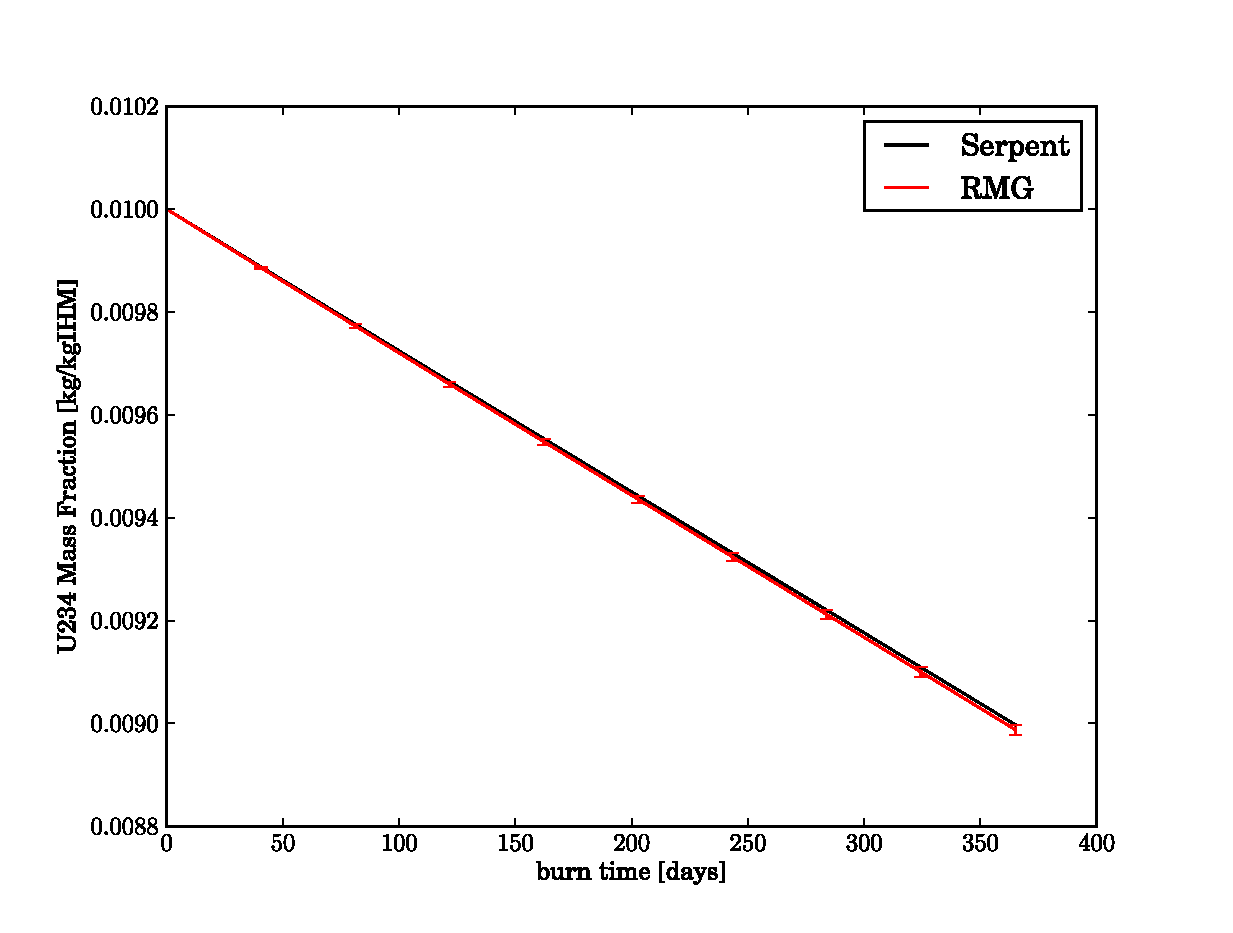
\includegraphics[scale=0.3]{multigroup_method/figs/benchmark/U234_Mass_Fraction_.eps}
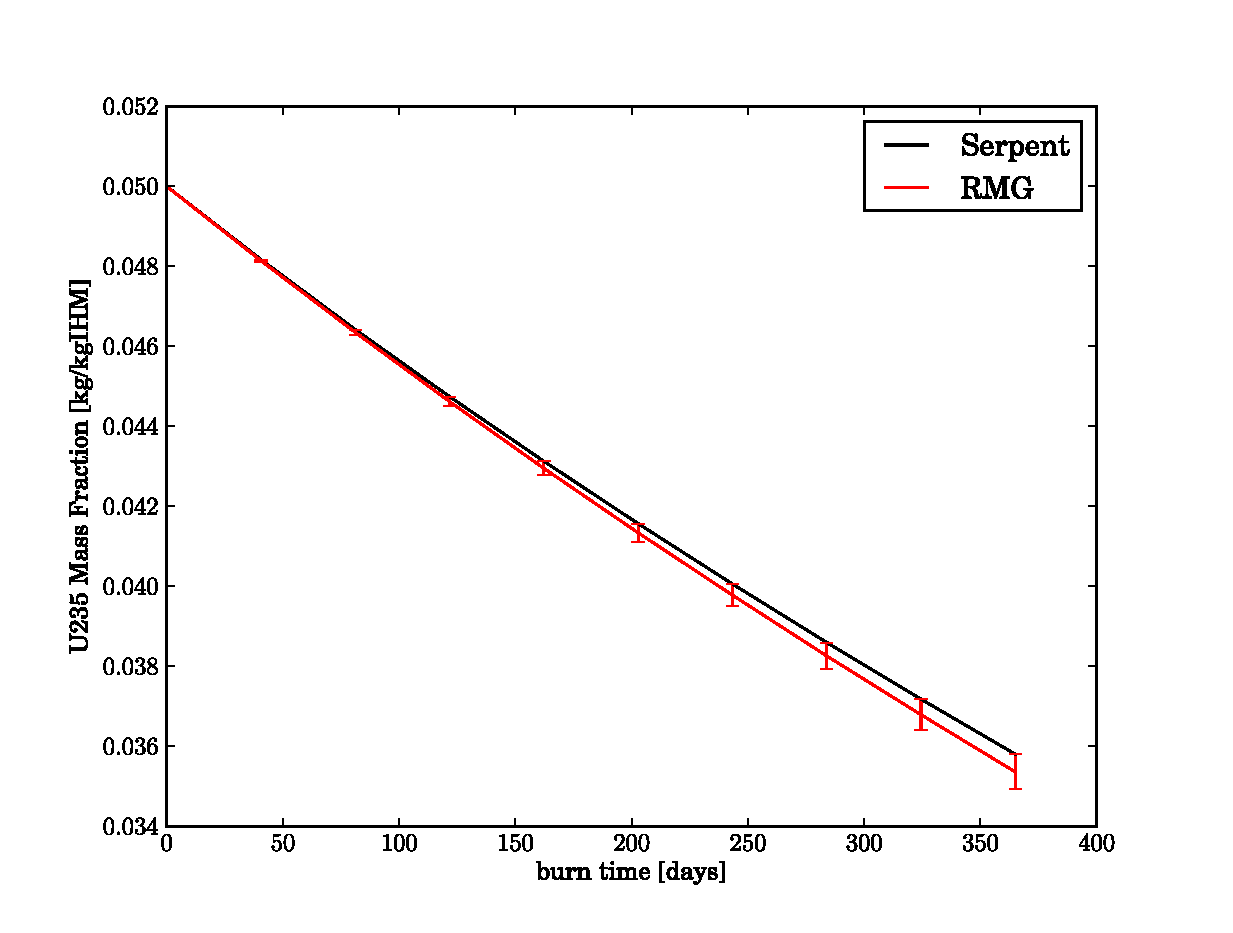
\includegraphics[scale=0.3]{multigroup_method/figs/benchmark/U235_Mass_Fraction_.eps}
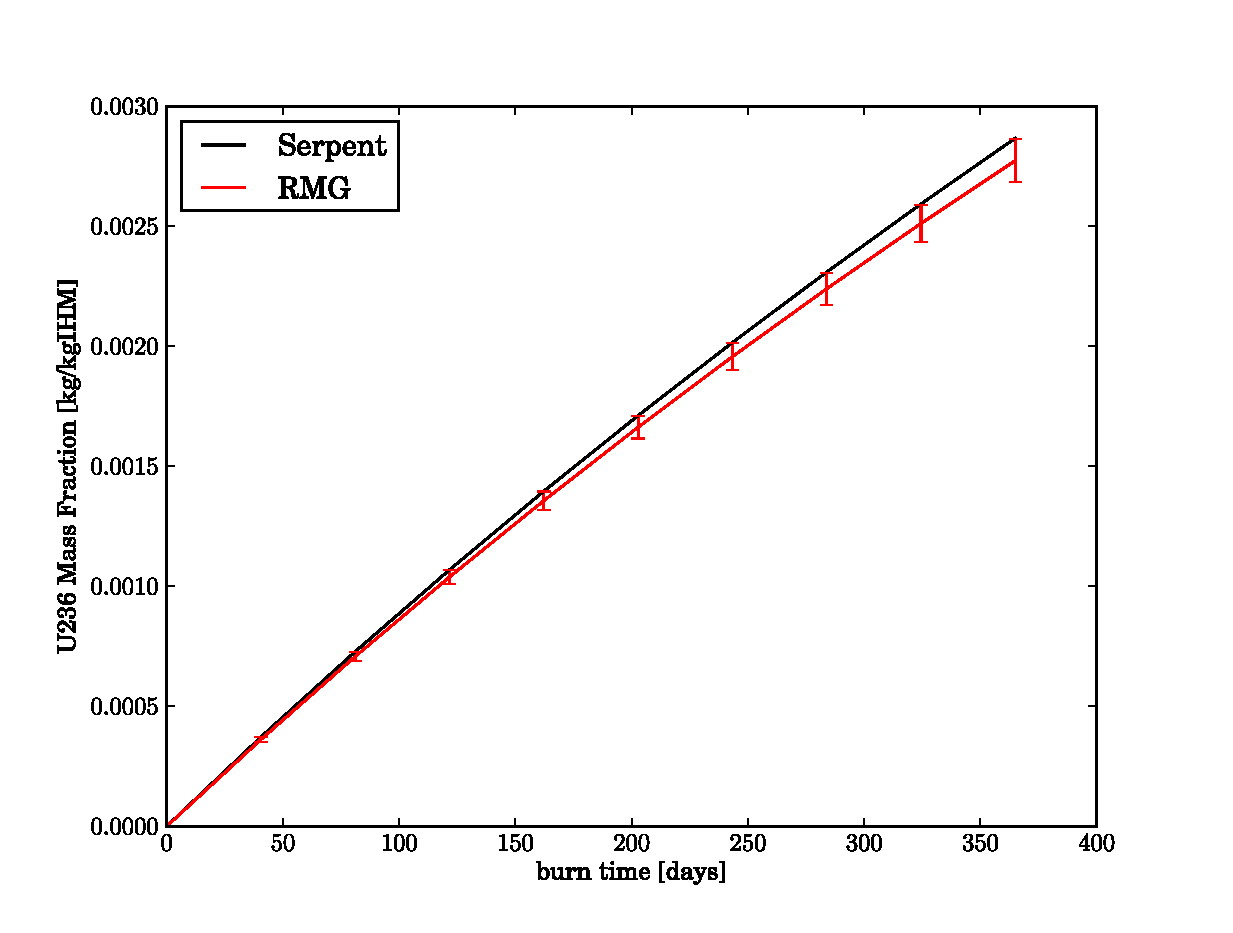
\includegraphics[scale=0.3]{multigroup_method/figs/benchmark/U236_Mass_Fraction_.eps}
\includegraphics[scale=0.3]{multigroup_method/figs/benchmark/U238_Mass_Fraction_.eps}
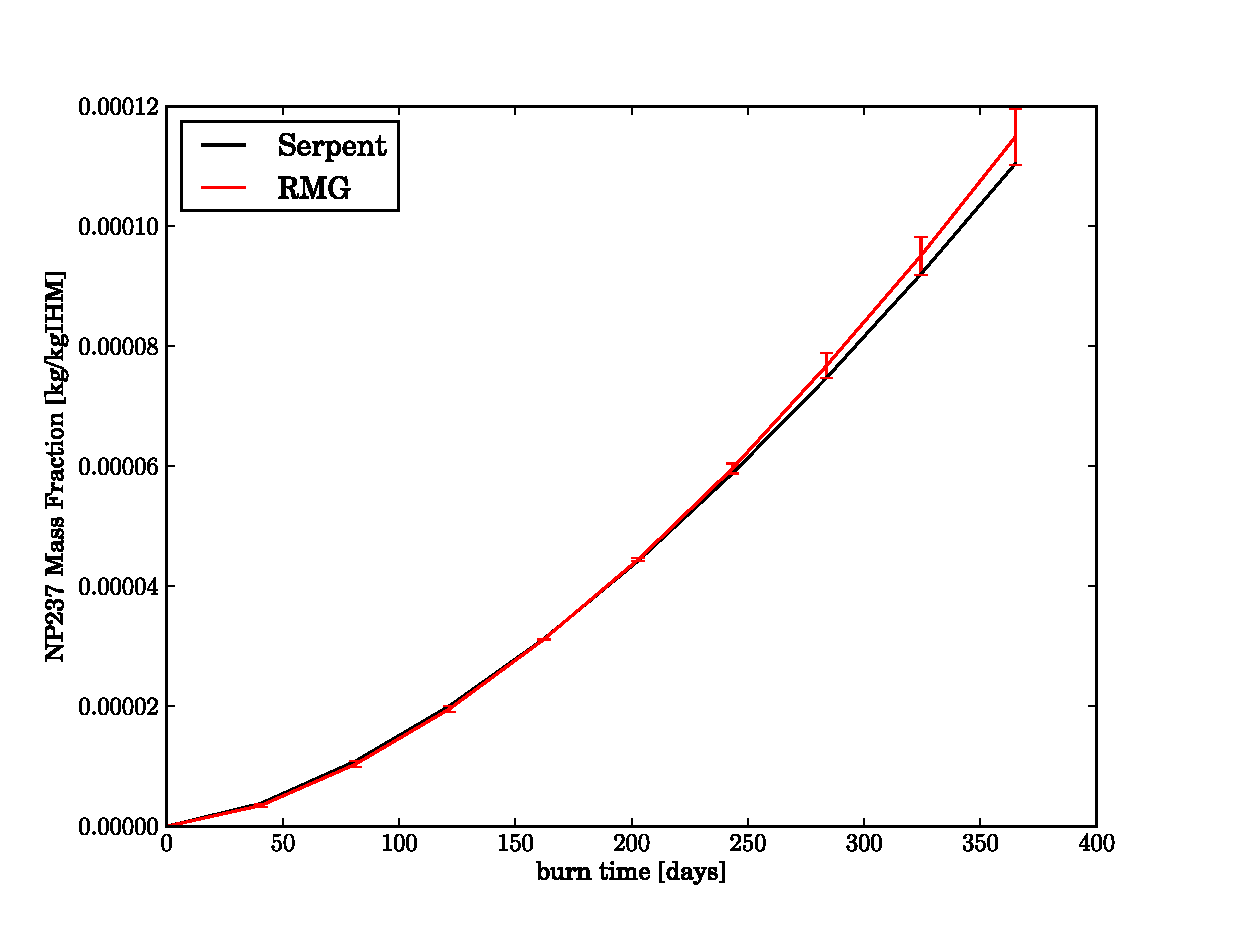
\includegraphics[scale=0.3]{multigroup_method/figs/benchmark/NP237_Mass_Fraction_.eps}
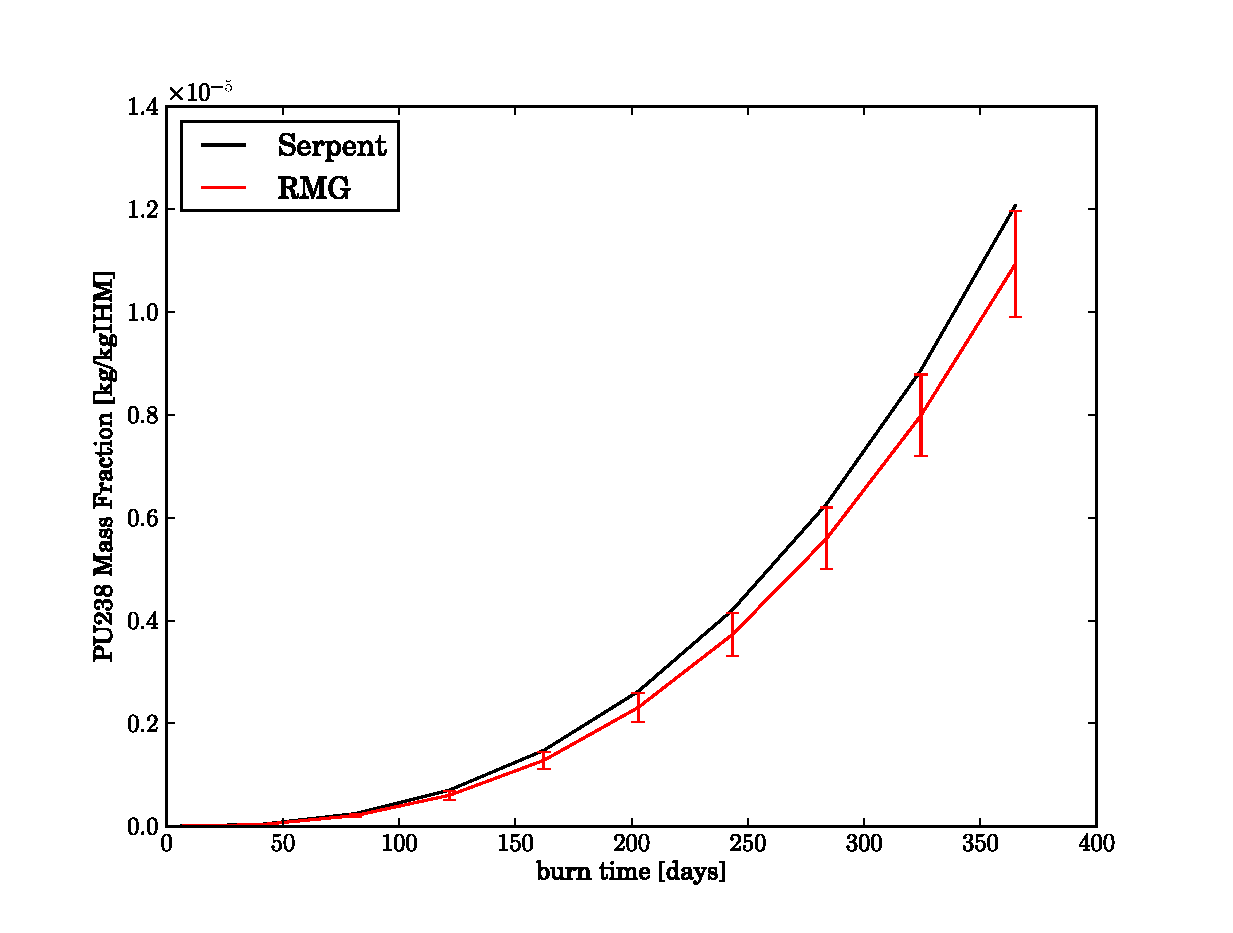
\includegraphics[scale=0.3]{multigroup_method/figs/benchmark/PU238_Mass_Fraction_.eps}
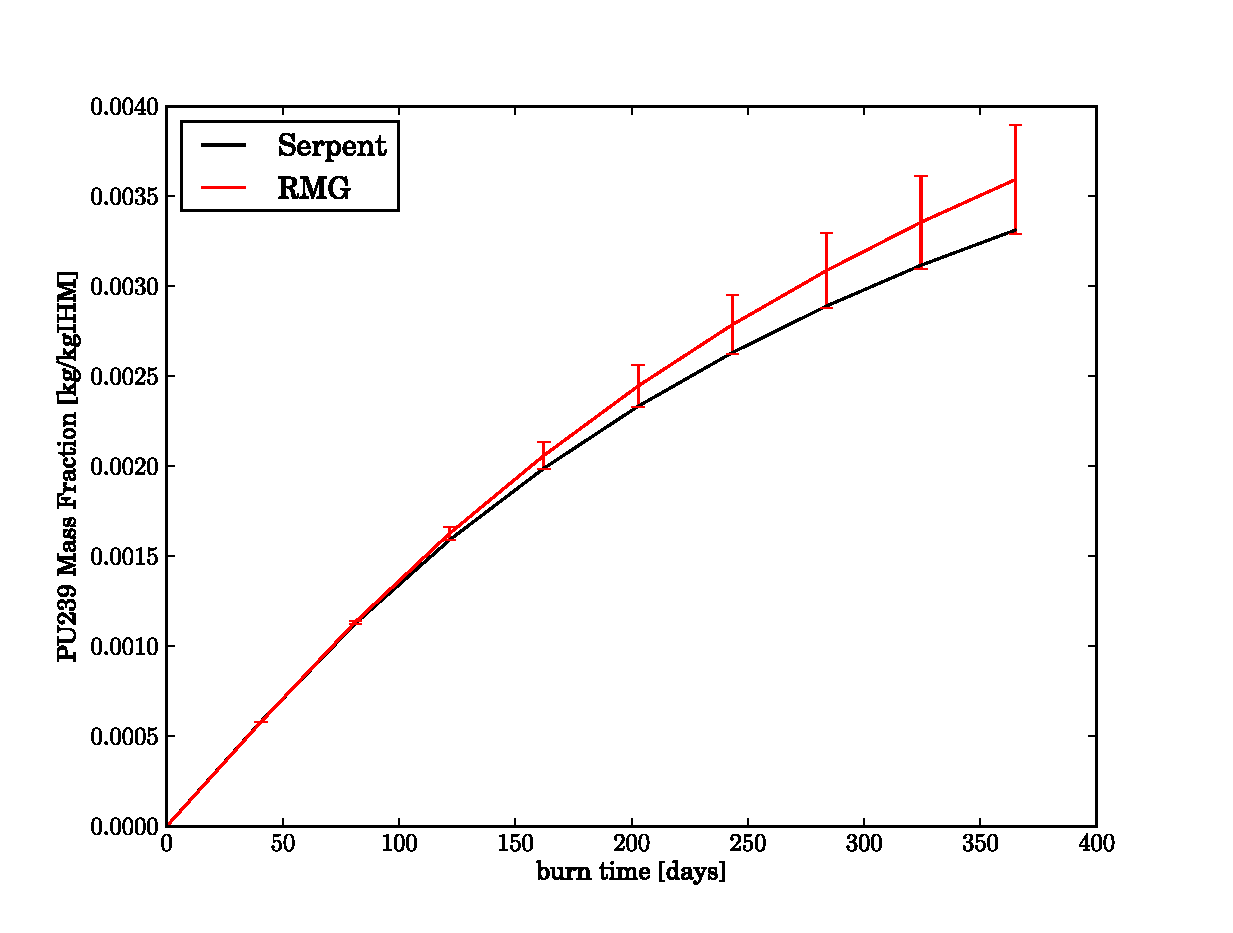
\includegraphics[scale=0.3]{multigroup_method/figs/benchmark/PU239_Mass_Fraction_.eps}
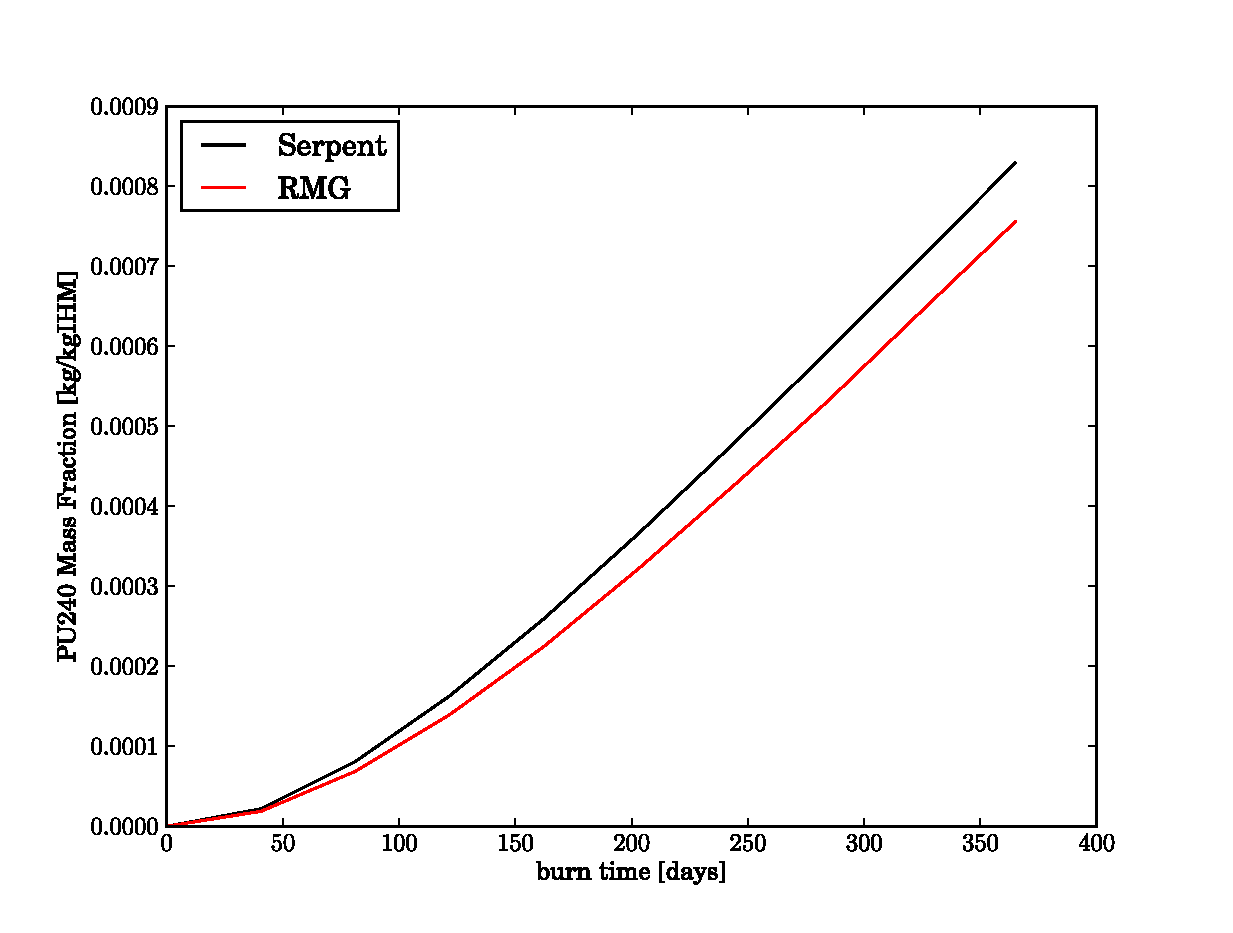
\includegraphics[scale=0.3]{multigroup_method/figs/benchmark/PU240_Mass_Fraction_.eps}
\end{center}
\end{figure}
\begin{figure}[htbp]
\caption{Actinide Mass Fraction Benchmarks (Cont.)}
\label{act_benchmark_cont}
\begin{center}
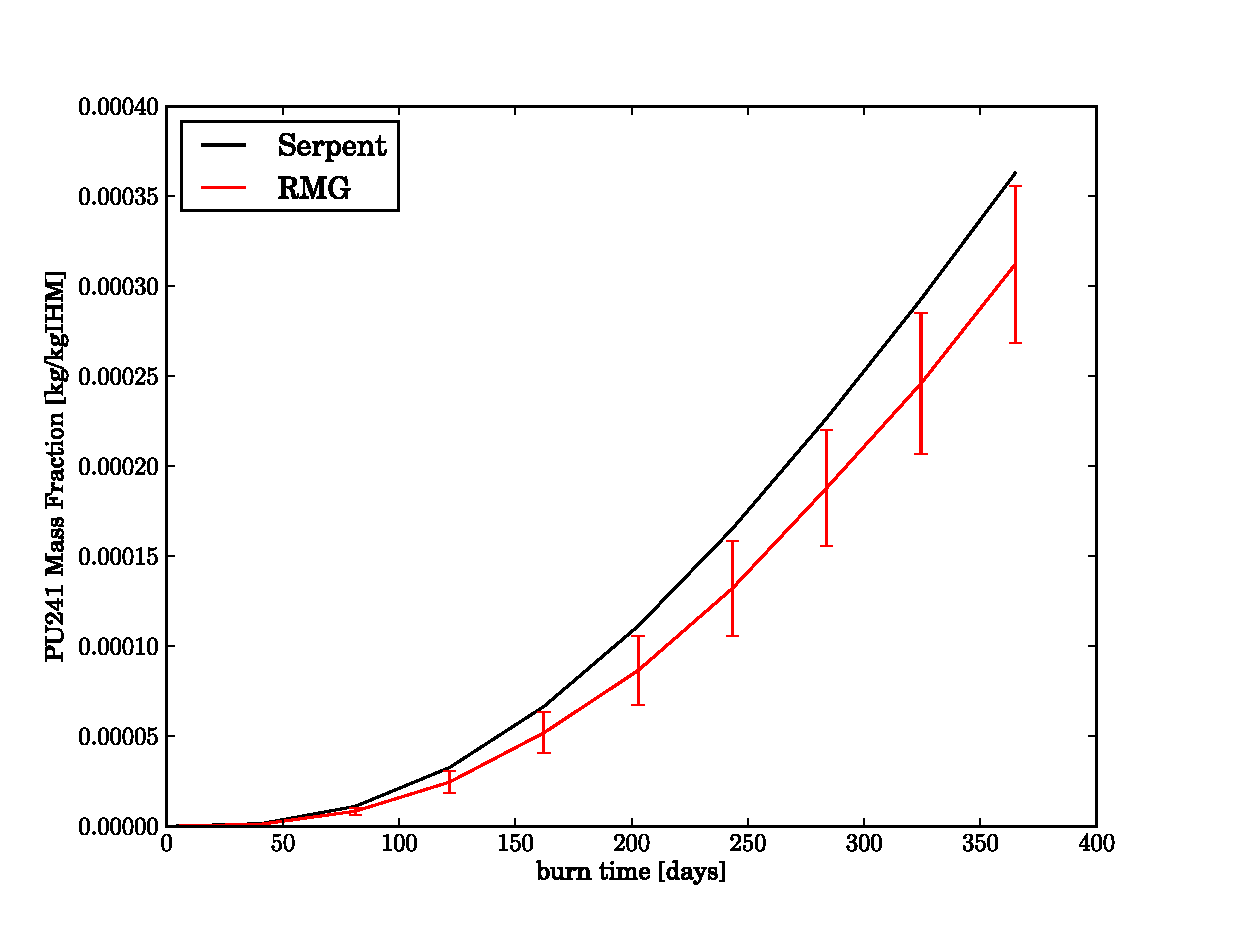
\includegraphics[scale=0.3]{multigroup_method/figs/benchmark/PU241_Mass_Fraction_.eps}
\includegraphics[scale=0.3]{multigroup_method/figs/benchmark/PU242_Mass_Fraction_.eps}
\includegraphics[scale=0.3]{multigroup_method/figs/benchmark/AM241_Mass_Fraction_.eps}
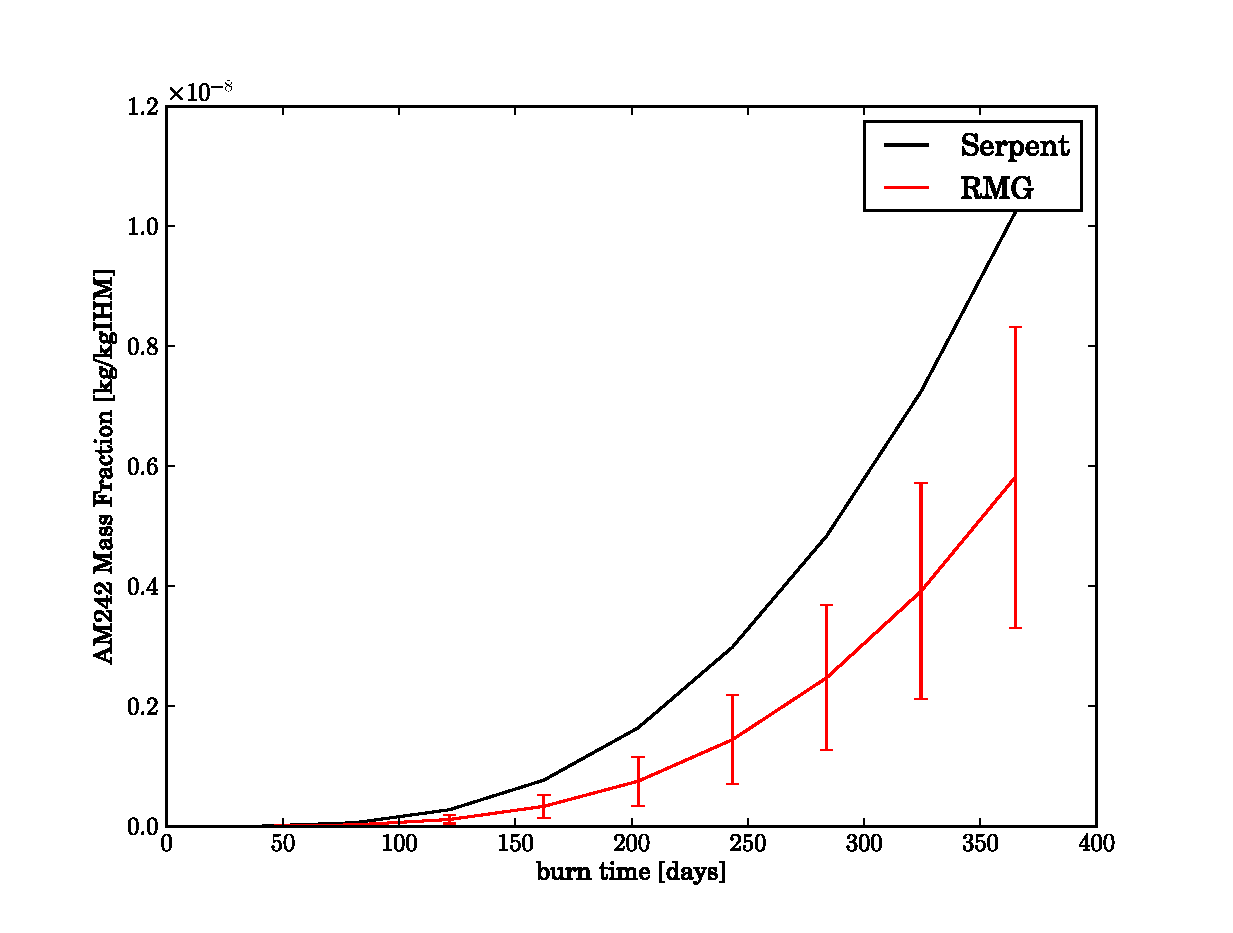
\includegraphics[scale=0.3]{multigroup_method/figs/benchmark/AM242_Mass_Fraction_.eps}
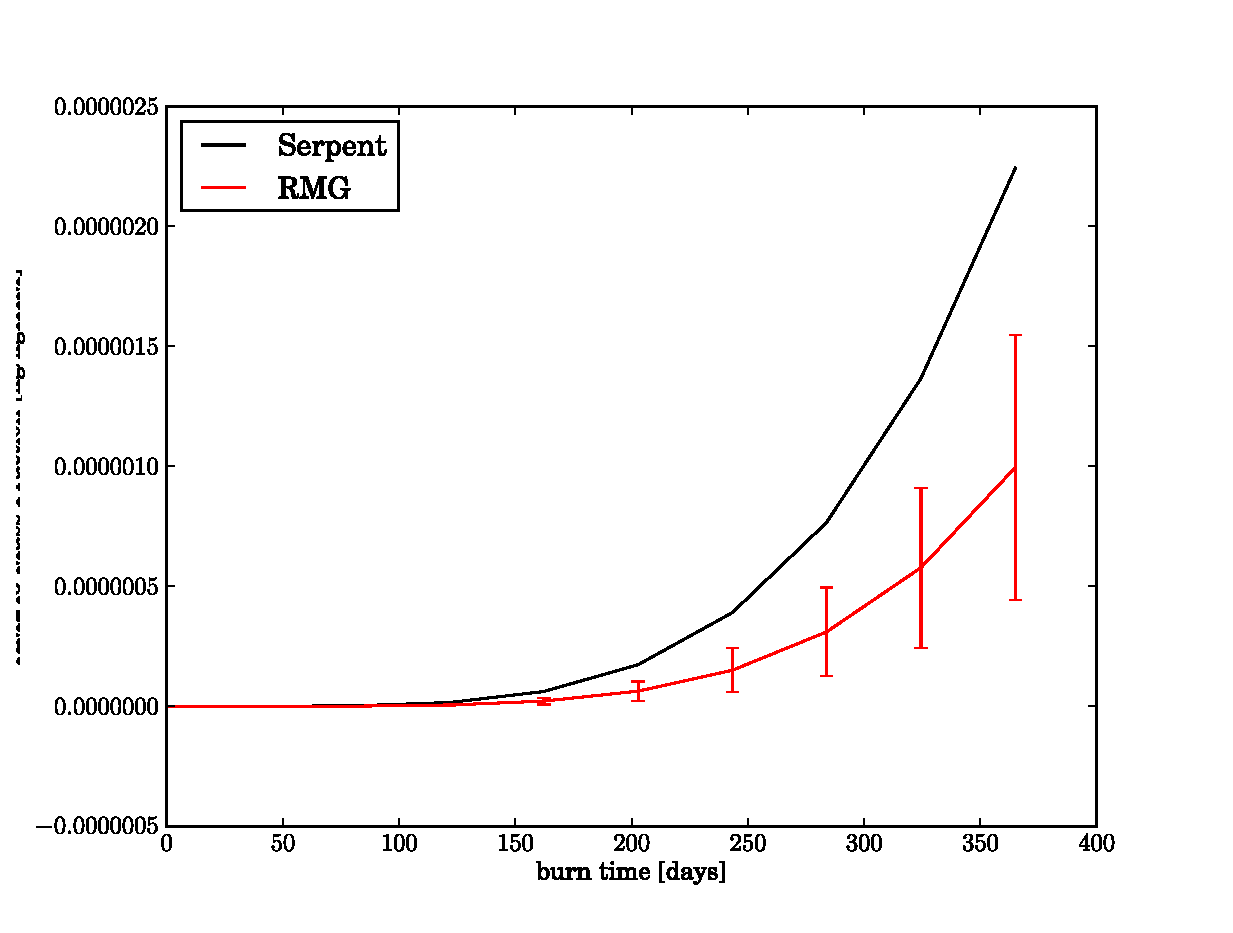
\includegraphics[scale=0.3]{multigroup_method/figs/benchmark/AM243_Mass_Fraction_.eps}
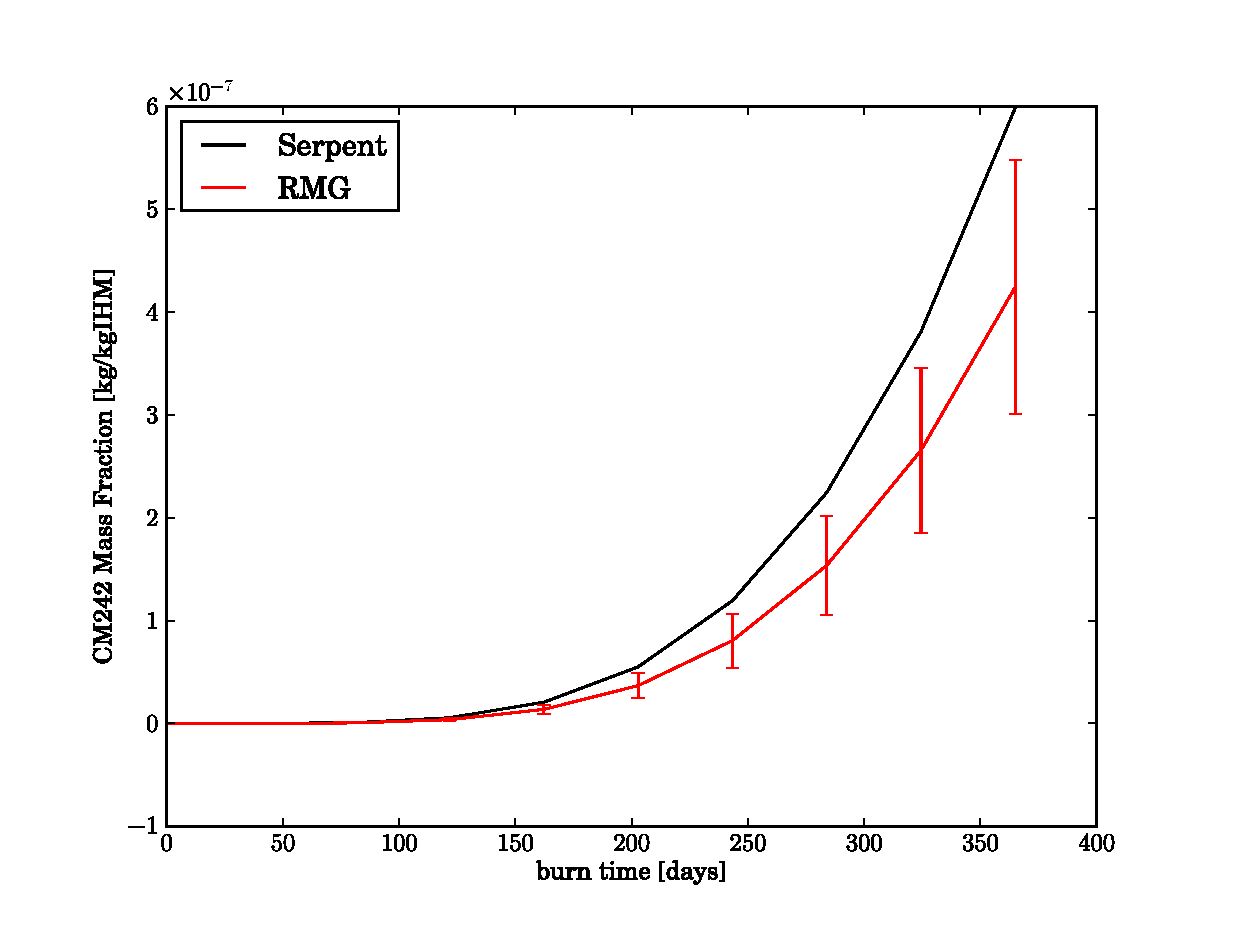
\includegraphics[scale=0.3]{multigroup_method/figs/benchmark/CM242_Mass_Fraction_.eps}
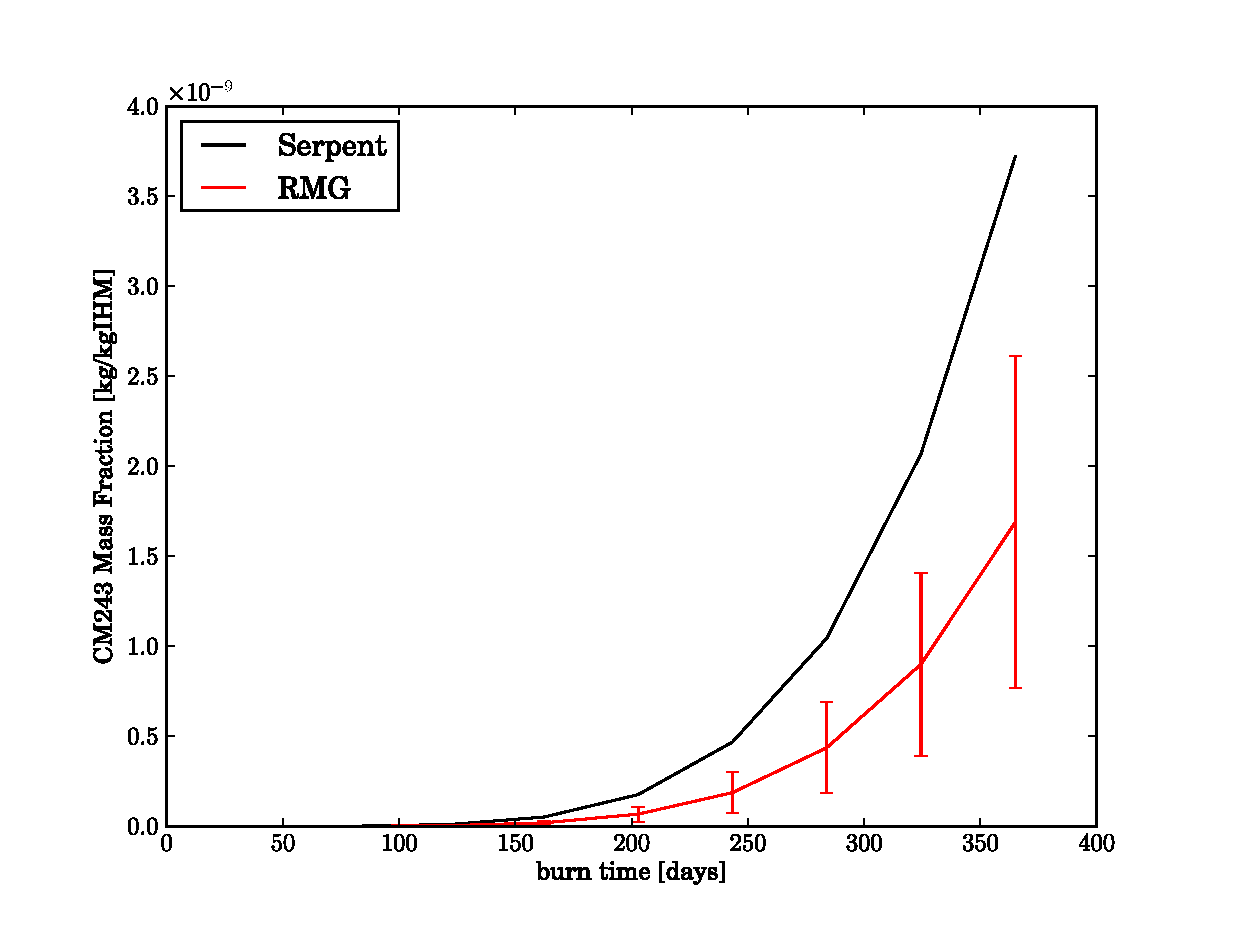
\includegraphics[scale=0.3]{multigroup_method/figs/benchmark/CM243_Mass_Fraction_.eps}
\includegraphics[scale=0.3]{multigroup_method/figs/benchmark/CM244_Mass_Fraction_.eps}
\end{center}
\end{figure}
\begin{figure}[htbp]
\caption{Actinide \& Fission Product Mass Fraction Benchmarks}
\label{act_fp_benchmark}
\begin{center}
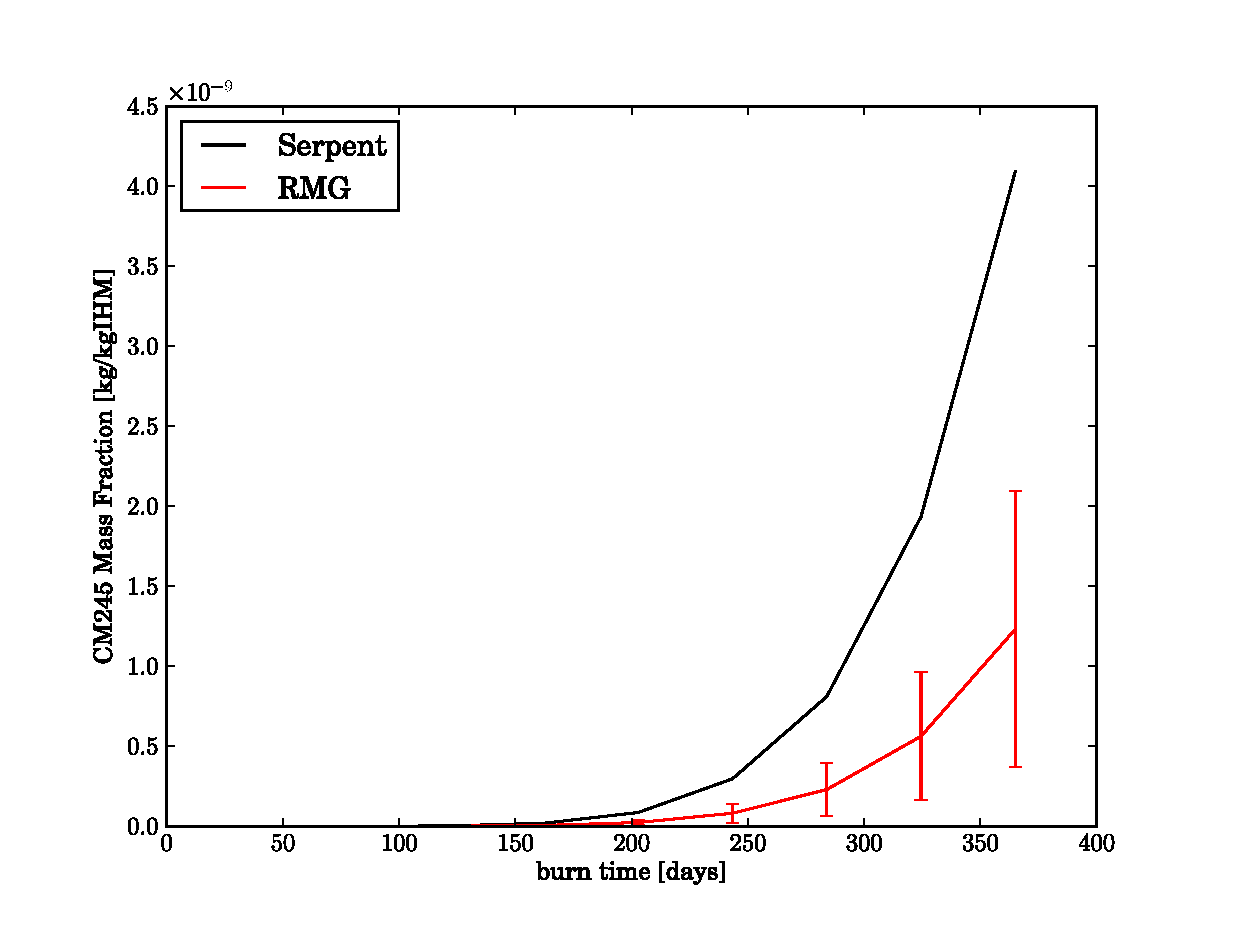
\includegraphics[scale=0.3]{multigroup_method/figs/benchmark/CM245_Mass_Fraction_.eps}
\includegraphics[scale=0.3]{multigroup_method/figs/benchmark/CM246_Mass_Fraction_.eps}
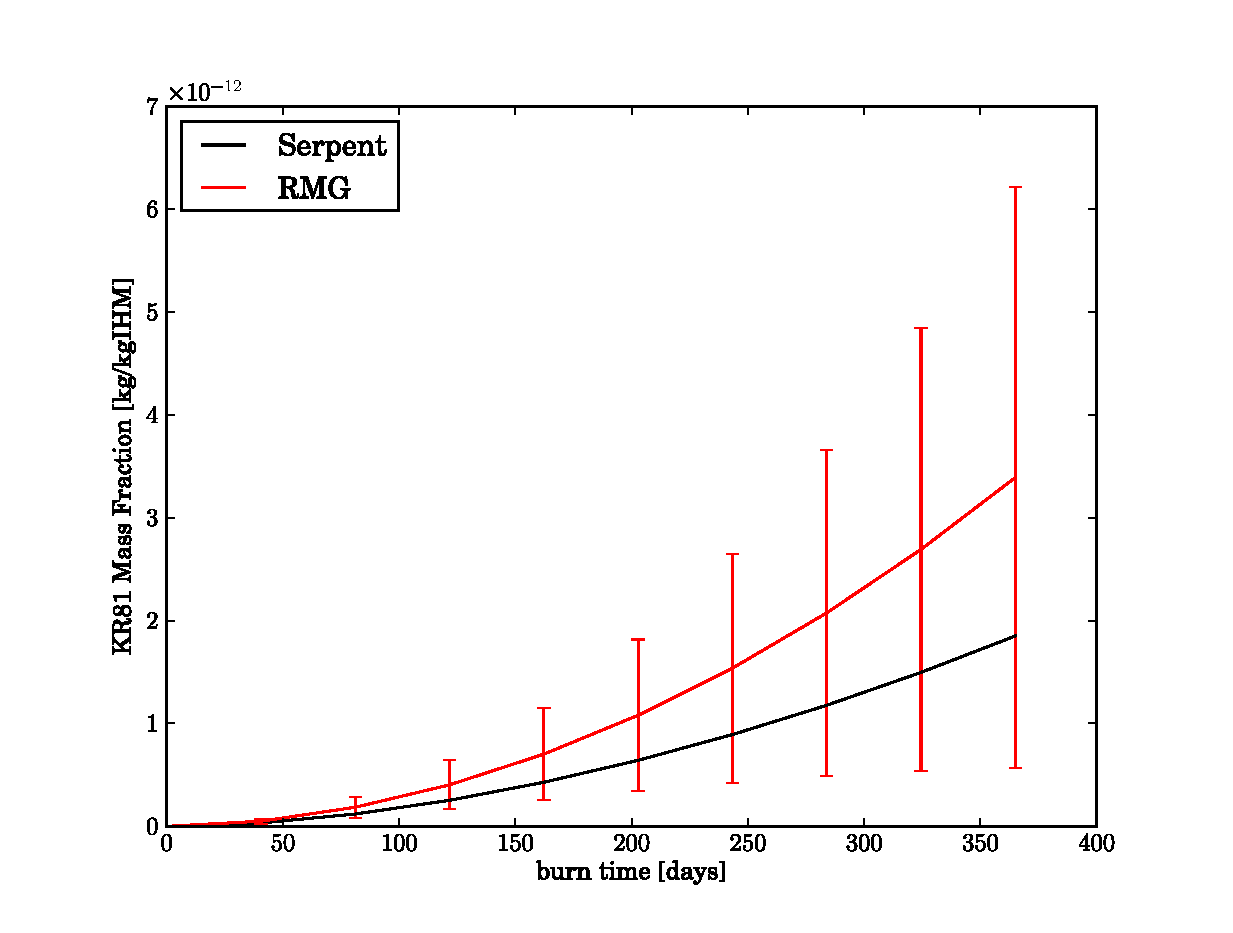
\includegraphics[scale=0.3]{multigroup_method/figs/benchmark/KR81_Mass_Fraction_.eps}
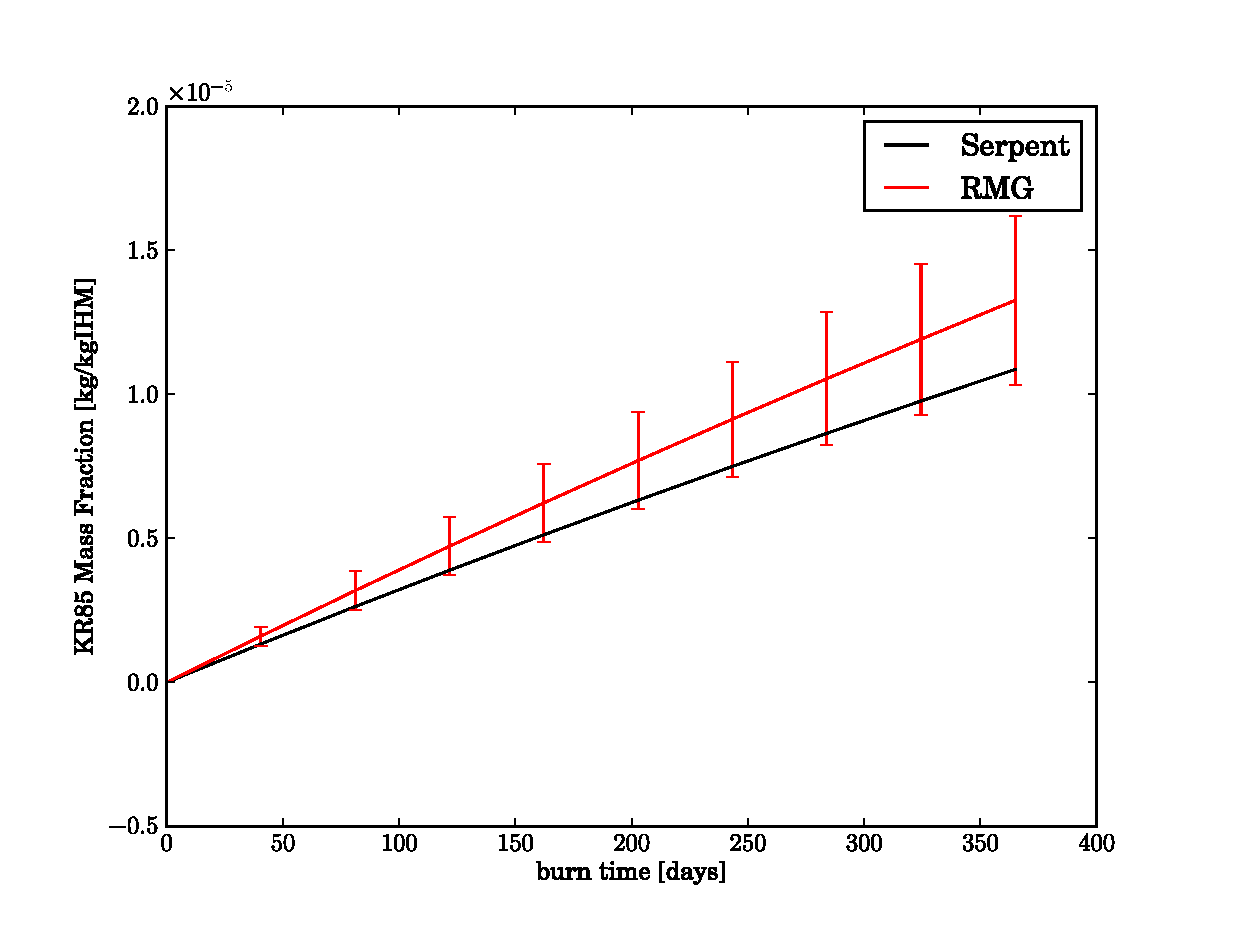
\includegraphics[scale=0.3]{multigroup_method/figs/benchmark/KR85_Mass_Fraction_.eps}
\includegraphics[scale=0.3]{multigroup_method/figs/benchmark/SR90_Mass_Fraction_.eps}
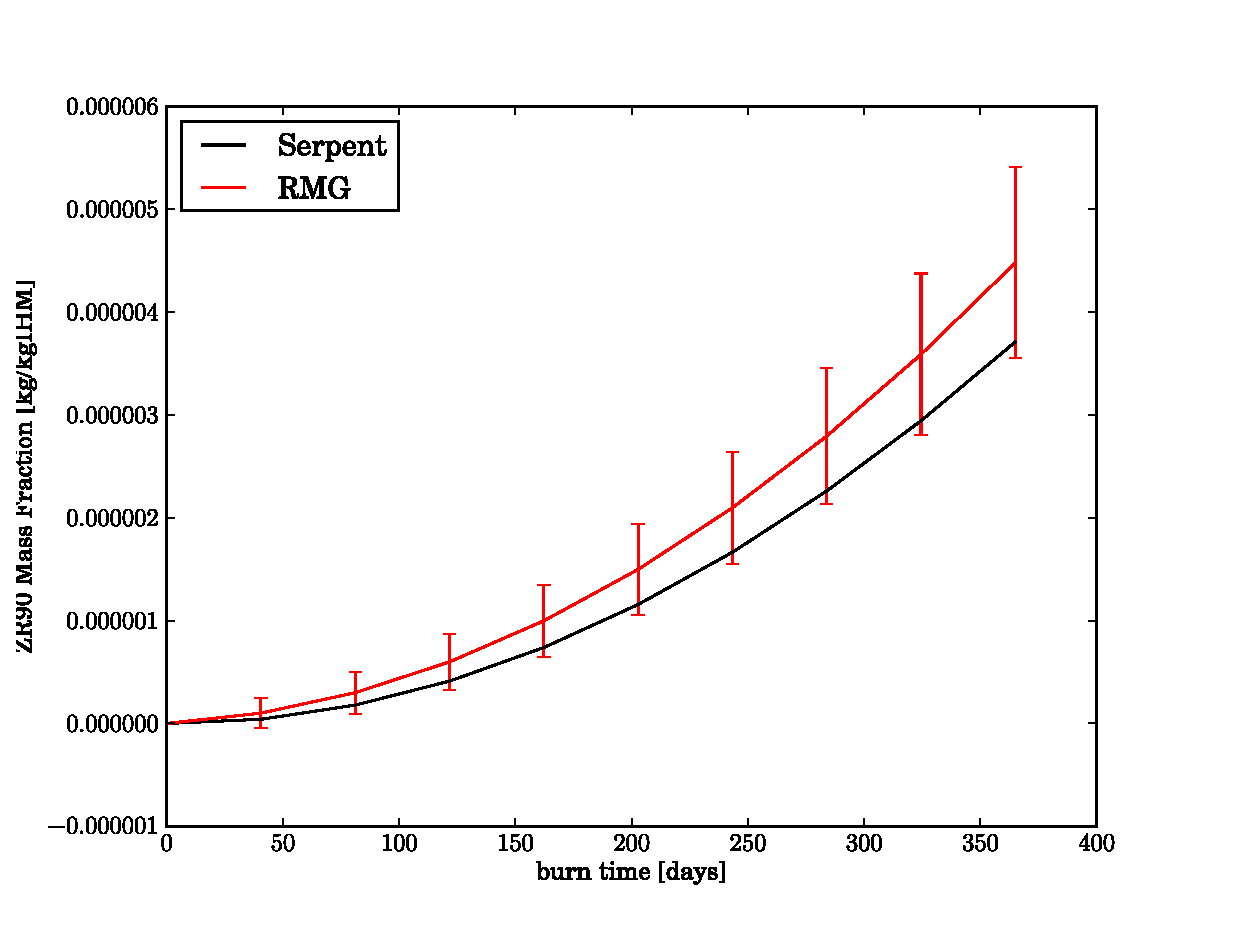
\includegraphics[scale=0.3]{multigroup_method/figs/benchmark/ZR90_Mass_Fraction_.eps}
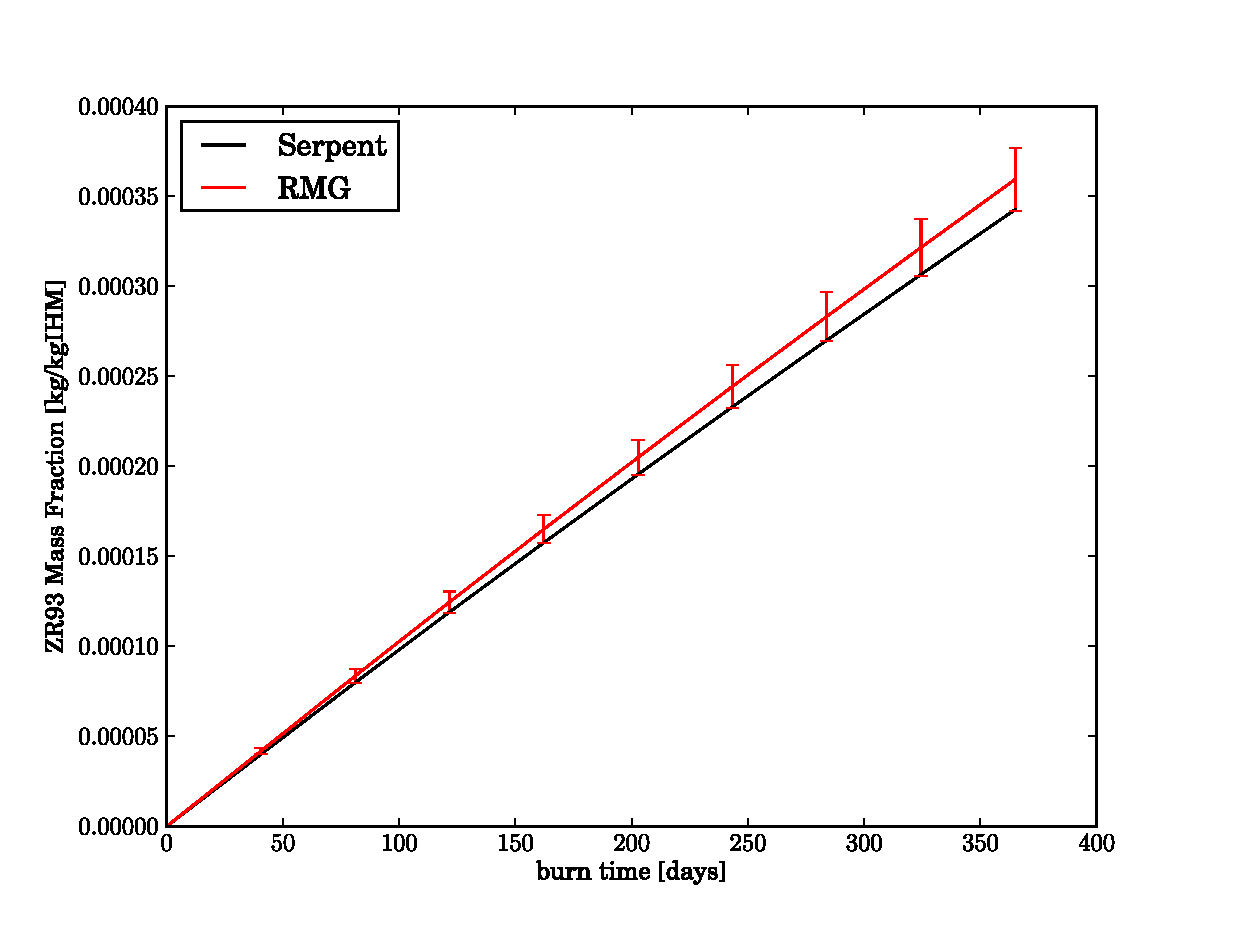
\includegraphics[scale=0.3]{multigroup_method/figs/benchmark/ZR93_Mass_Fraction_.eps}
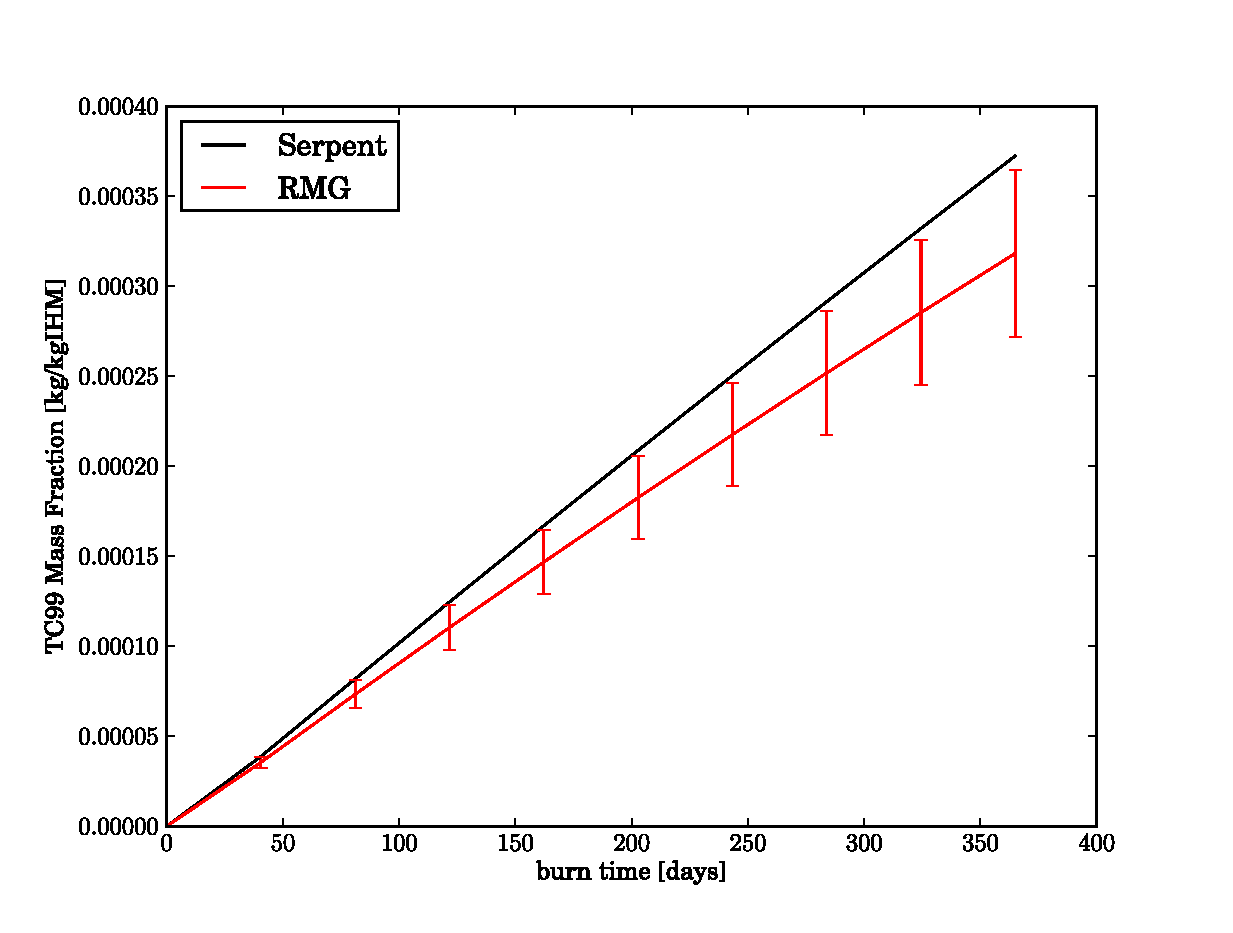
\includegraphics[scale=0.3]{multigroup_method/figs/benchmark/TC99_Mass_Fraction_.eps}
\end{center}
\end{figure}
\begin{figure}[htbp]
\caption{Fission Product Mass Fraction Benchmarks (Cont.)}
\label{act_fp_benchmark_cont}
\begin{center}
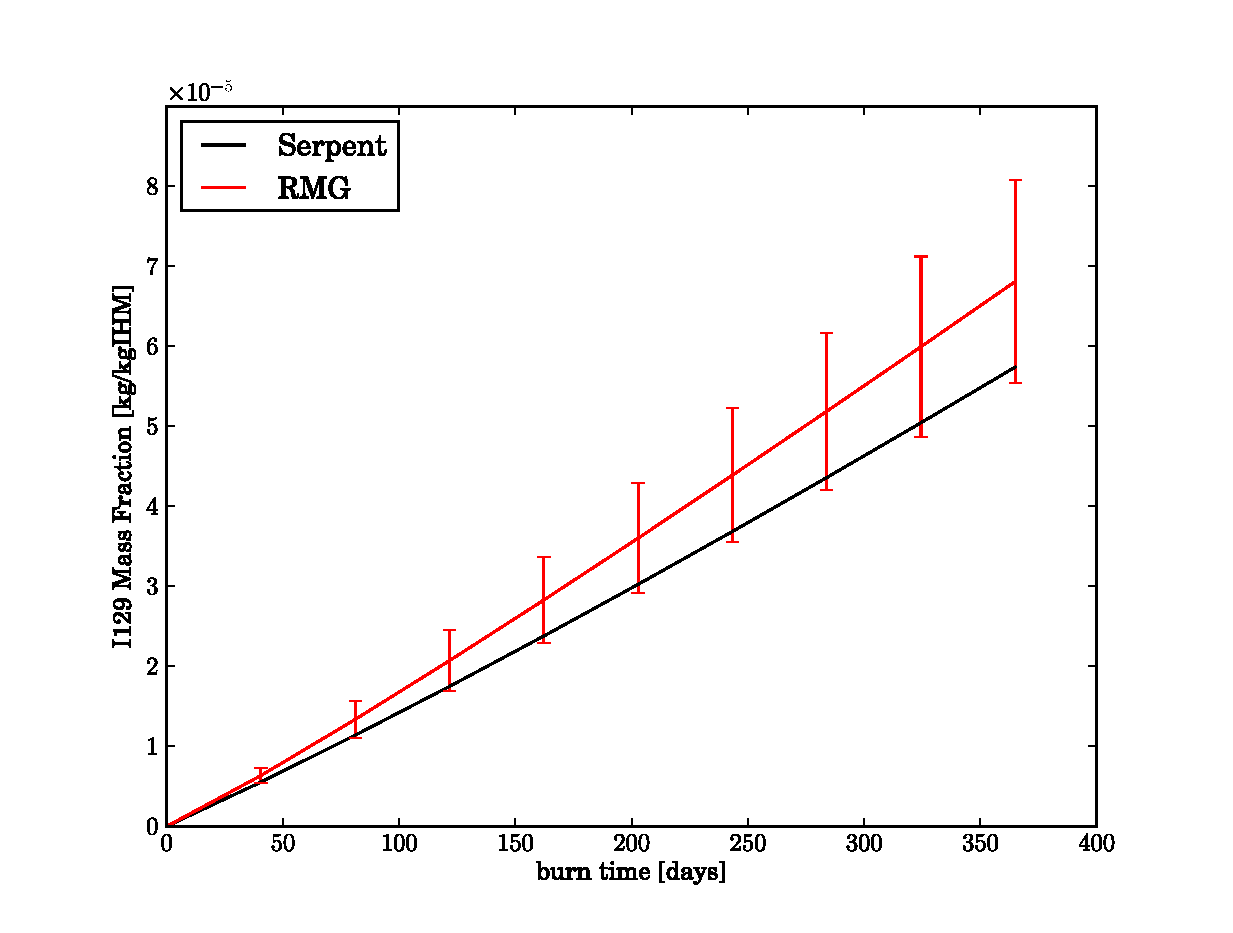
\includegraphics[scale=0.3]{multigroup_method/figs/benchmark/I129_Mass_Fraction_.eps}
\includegraphics[scale=0.3]{multigroup_method/figs/benchmark/PD107_Mass_Fraction_.eps}
\includegraphics[scale=0.3]{multigroup_method/figs/benchmark/CS134_Mass_Fraction_.eps}
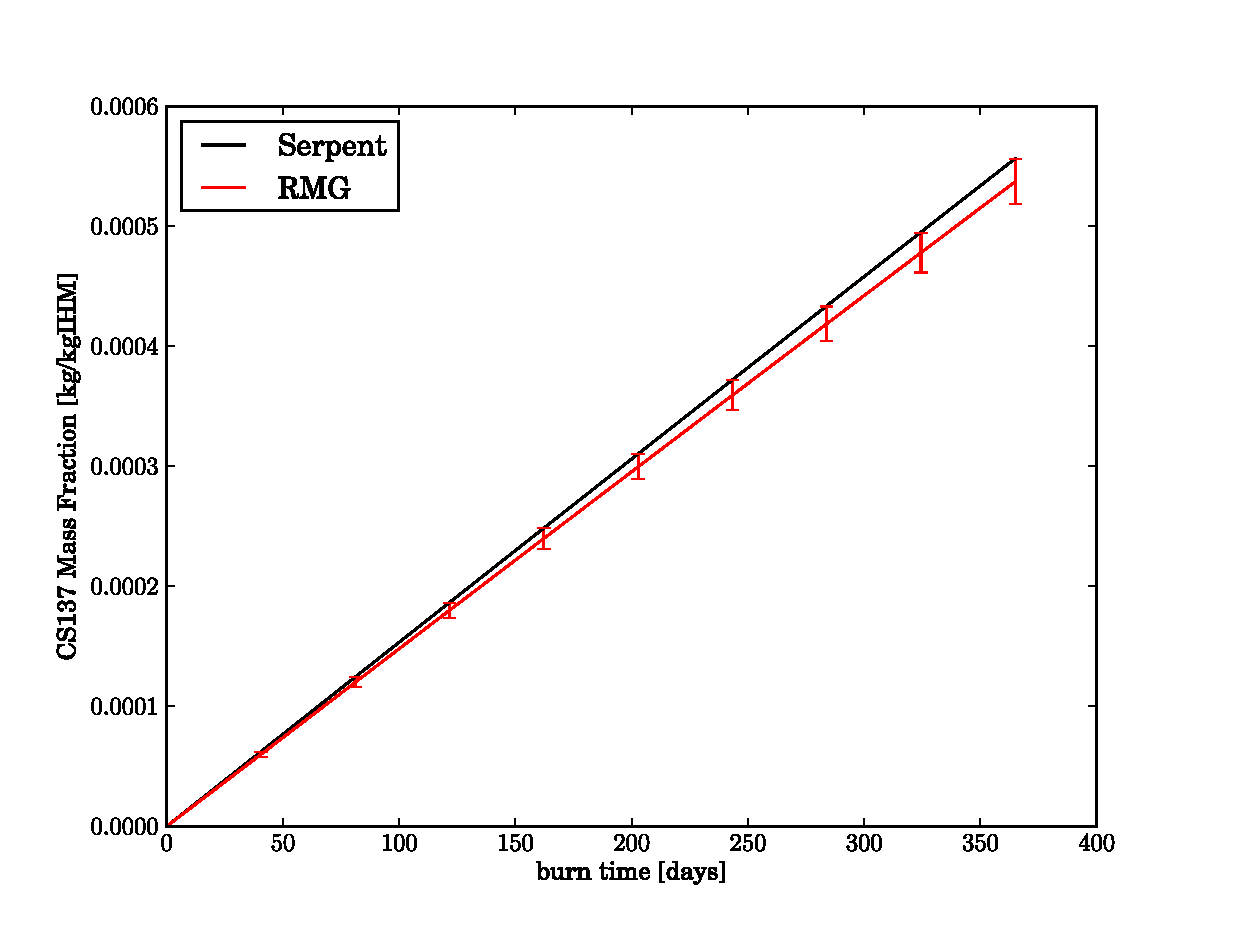
\includegraphics[scale=0.3]{multigroup_method/figs/benchmark/CS137_Mass_Fraction_.eps}
\end{center}
\end{figure}


As is seen in these figures, there is good agrement between the transmutation vectors computed by
Serpent and those computed by the RMG via Origen.  The instances with non-trivial disagreements are 
largely in the higher order actinides.  These nuclides exist in such small amounts, that the relatively
high errors do not adeversely effect the neutronic performance of the fuel.

However, the true strength of the RMG methodology is 
that it takes into account the time evolotion of the cross sections as well.  For the same set 
of nuclides above, Figures XXX - XXX display total, absorption, scattering and fission one-group 
cross sections as a function of burn time.  One-group cross sections are used here in favor 
of the multigroup cross sections because they capture the total differences between data sets 
while removing the complexity of plotting three dimensional information.

XXX - Add 1G XS figures here.

Lastly, since the one-group cross sections are feed to Origen to make a transmutation library, it is important 
to ensure that no library is reaction is far off from a benchmark value.  Tables XXX - XXX display the 
nuclides with the highest $\varepsilon$ (in decending order) at any time step for absorption and scattering
reactions for the fission products and for absorption, scattering and fission reactions for the actinides.
These tables have been filtered to remove species that have very short half lives within the reactor.
As Tables XXX - XXX display, even in the worst case the cross sections meet within acceptable levels or error.

\section{Conclusion \& Future Work}
\index{Conclusion \& Future Work@\emph{Conclusion \& Future Work}}
Do it!



%\include{chapter-howtouse}

%\include{chapter-makingbib}

%\include{chapter-tables+figs}

%\include{chapter-math}


%%%%%%%%%%%%%%%%%%%%%%%%%%%%%%%%%%%%%%%%%%%%%%%%%%%%%%%%%%%%%%%%%%%%%%
% Appendix/Appendices                                                %
%%%%%%%%%%%%%%%%%%%%%%%%%%%%%%%%%%%%%%%%%%%%%%%%%%%%%%%%%%%%%%%%%%%%%%
%
% If you have only one appendix, use the command \appendix instead
% of \appendices.
%
\appendices
\index{Appendices@\emph{Appendices}}%

\chapter{Serpent Input Decks}
\index{Appendix!Serpent Input Decks@\emph{Serpent Input Decks}}
\label{appendix_serpent_input}

The following displays sample Serpent input input decks that were used in the benchmark 
case for the multigroup model.  Serpent was run in both burnup and cross section generation 
modes.  Both files are for the reactor at the beginning of life.  First, a sample burnup file 
is presented below.  

\vspace{1em}

\lstinputlisting[language=Matlab, caption={Serpent Burnup Input Deck}, label=serpent_input_burnup]{multigroup_method/figs/serpent_input_burnup}

\vspace{1em}

Next follows a Serpent input deck that was used to compute the \nuc{U}{238} group constants. 
Input files for other nuclides follow analogously.

\vspace{1em}

\lstinputlisting[language=Matlab, caption={Serpent Cross Section Input Deck}, label=serpent_input_xs_gen]{multigroup_method/figs/serpent_input_xs_gen}



\chapter{Integration of Double Differential Scattering Cross Section Over Solid Angle}
\index{Appendix!Integration of Double Differential Scattering Cross Section Over Solid Angle@\emph{Integration of Double Differential Scattering Cross Section Over Solid Angle}}
\label{appendix_integrate_solid_angle}

Suppose that equation \ref{app_scat_ce} is a continuous energy, double differential model of the scattering
cross section \cite{Yamamoto2006, Mattes2005}.
\begin{equation}
\label{app_scat_ce}
\frac{d^2}{dE^\prime d\Omega} \sigma_s(E\to E^\prime, \Omega\to\Omega^\prime) = \frac{b^2}{kT} \cdot
            %\left(1 - \frac{2E}{931.46 \cdot m_n}\right) \cdot
            \sqrt{\frac{E^{\prime}}{E}} e^{-\frac{\beta}{2}} S(\alpha, \beta)
\end{equation}
where $b$ [cm] is the bound scattering length of the target nucleus, $E$ [MeV] is the incident
neutron energy, $E^\prime$ [MeV] is exiting neutron energy, $\Omega$ [sr] is the incident
neutron solid angle, $\Omega^\prime$ [sr] is the exiting neutron solid angle,
$m_n$ is mass of the neutron,
$M_A$ is the mass of the target nucleus, and $k$ [MeV/K] is Boltzmann's constant.  Note that the term 
$S(\alpha, \beta)$ is the scattering kernel with the scattering parameters $\alpha$ and $\beta$.
\begin{equation}
\label{app_scat_alpha}
\alpha = \frac{E^\prime + E - 2\sqrt{E^\prime E}\cos(\theta)}{\frac{M_A}{m_n}kT}
\end{equation}
\begin{equation}
\label{app_scat_beta}
\beta = \frac{E^\prime - E}{kT}
\end{equation}
Using the free gas approximation, $S(\alpha, \beta)$ is modeled as seen in equation \ref{app_scat_kern}.
\begin{equation}
\label{app_scat_kern}
S(\alpha, \beta) = \frac{1}{\sqrt{4\pi\alpha}} \mbox{Exp}\left(-\frac{\alpha^2 + \beta^2}{4\alpha}\right)
\end{equation}
By integrating the double differential scattering cross section over all solid angles $\Omega$, 
an energy-only expression may be obtained.

Begin by noting that the only term in equation \ref{app_scat_ce} that is dependent on the 
scattering angle is the kernel $S(\alpha, \beta)$.  Thus defining $K$ such that, 
\begin{equation}
\label{app_big_k}
K = \frac{b^2}{kT} \sqrt{\frac{E^{\prime}}{E}}
\end{equation}
equation \ref{app_scat_ce} becomes equation \ref{app_scat_ke}.
\begin{equation}
\label{app_scat_ke}
\frac{d^2}{dE^\prime d\Omega} \sigma_s(E\to E^\prime, \Omega\to\Omega^\prime) = K \cdot
                e^{-\frac{\beta}{2}} \cdot
                \frac{e^{-\frac{\alpha^2 + \beta^2}{4\alpha}}}{\sqrt{4\pi\alpha}}
\end{equation}
This expression in turn may be integrated over all scattering angle, on which only $\alpha$ 
is dependent for a free gas.
\begin{equation}
\label{app_int_ke}
\frac{d\sigma_s(E\to E^\prime)}{dE^\prime} = K \cdot
                e^{-\frac{\beta}{2}} \cdot
                \int_\Omega \frac{e^{-\frac{\alpha^2 + \beta^2}{4\alpha}}}{\sqrt{4\pi\alpha}} d\Omega
\end{equation}
Expanding the $\Omega$ into its azimuthal and inclination angle components, the integral in 
equation \ref{app_int_ke} may be reduced as follows.
\begin{equation}
\label{app_int_ke_1}
\int_\Omega \frac{e^{-\frac{\alpha^2 + \beta^2}{4\alpha}}}{\sqrt{4\pi\alpha}} d\Omega = 
    \int_0^{2\pi} \int_0^\pi \frac{e^{-\frac{\alpha^2 + \beta^2}{4\alpha}}}{\sqrt{4\pi\alpha}} \sin(\theta) d\theta d\phi = 
    2\pi \int_0^\pi \frac{e^{-\frac{\alpha^2 + \beta^2}{4\alpha}}}{\sqrt{4\pi\alpha}} \sin(\theta) d\theta
\end{equation}
Now making a change of variables by setting $\mu=\cos(\theta)$, the integral in equation \ref{app_int_ke_1}
becomes, 
\begin{equation}
\label{app_int_ke_2}
\sqrt{\pi} \int_1^{-1} \frac{e^{-\frac{\alpha^2 + \beta^2}{4\alpha}}}{\sqrt{\alpha}} \sin(\theta) \frac{-d\mu}{\sin(\theta)} = 
                \sqrt{\pi} \int_{-1}^1 \frac{e^{-\frac{\alpha^2 + \beta^2}{4\alpha}}}{\sqrt{\alpha}} d\mu
\end{equation}
Performing another change of variables from $\mu$ to $\alpha$, the relationship $L$ is found between
the differentials.
\begin{equation}
\label{app_dmu_dalpha}
\frac{d\mu}{d\alpha} = - \frac{2\sqrt{E^\prime E}}{\frac{M_A}{m_n}kT} = L
\end{equation}
The limits on the integrand are thus defined as follows.
\begin{equation}
\label{app_alpha_limits}
\alpha_{\pm 1} = \frac{E^\prime + E \mp 2\sqrt{E^\prime E}}{\frac{M_A}{m_n}kT}
\end{equation}
Thus the evaluation of the integral becomes dependent on the error function.
\begin{equation}
\label{app_int_ke_3}
\frac{\sqrt{\pi}}{L} \int_{\alpha_{-1}}^{\alpha_1} \frac{e^{-\frac{\alpha^2 + \beta^2}{4\alpha}}}{\sqrt{\alpha}} d\alpha = 
    \frac{\pi}{L} e^{-\frac{|\beta|}{2}} \left. \left(
    e^{|\beta|} \mbox{Erf}\left[\frac{|\beta| + \alpha}{2\sqrt{\alpha}}\right] - 
    \mbox{Erf}\left[\frac{|\beta| - \alpha}{2\sqrt{\alpha}}\right] - 
    e^{|\beta|} + 1
    \right) \right|_{\alpha_{-1}}^{\alpha_1}
\end{equation}
The terms in this evaluation that are not dependent on $\alpha$ disappear when the limits are applied.
\begin{equation}
\label{app_int_ke_4}
\frac{\sqrt{\pi}}{L} \int_{\alpha_{-1}}^{\alpha_1} \frac{e^{-\frac{\alpha^2 + \beta^2}{4\alpha}}}{\sqrt{\alpha}} d\alpha = 
    \frac{\pi}{L} \left. \left(
    e^{\frac{|\beta|}{2}}  \mbox{Erf}\left[\frac{|\beta| + \alpha}{2\sqrt{\alpha}}\right] - 
    e^{-\frac{|\beta|}{2}} \mbox{Erf}\left[\frac{|\beta| - \alpha}{2\sqrt{\alpha}}\right] 
    \right) \right|_{\alpha_{-1}}^{\alpha_1}
\end{equation}
Adding in the $e^{-\frac{\beta}{2}}$ term from equation \ref{app_int_ke}, 
\begin{equation}
\label{app_int_ke_5}
e^{-\frac{\beta}{2}} \frac{\sqrt{\pi}}{L} \int_{\alpha_{-1}}^{\alpha_1} \frac{e^{-\frac{\alpha^2 + \beta^2}{4\alpha}}}{\sqrt{\alpha}} d\alpha = 
    \frac{\pi}{L} \left. \left(
    e^{-\frac{\beta - |\beta|}{2}} \mbox{Erf}\left[\frac{|\beta| + \alpha}{2\sqrt{\alpha}}\right] - 
    e^{-\frac{\beta + |\beta|}{2}} \mbox{Erf}\left[\frac{|\beta| - \alpha}{2\sqrt{\alpha}}\right] 
    \right) \right|_{\alpha_{-1}}^{\alpha_1}
\end{equation}
This expression may be further simplified to 
\begin{equation}
\label{app_int_ke_6}
e^{-\frac{\beta}{2}} \frac{\sqrt{\pi}}{L} \int_{\alpha_{-1}}^{\alpha_1} \frac{e^{-\frac{\alpha^2 + \beta^2}{4\alpha}}}{\sqrt{\alpha}} d\alpha = 
    \frac{\pi}{L} \left(Q^+(\alpha, \beta) - Q^-(\alpha, \beta) \right) 
\end{equation}
by defining a $Q$ such that
\begin{equation}
\label{app_Q_pm}
Q^\pm(\alpha, \beta) = e^{-\frac{\beta \mp |\beta|}{2}} \left( 
    \mbox{Erf}\left[\frac{|\beta| \pm \alpha_1}{2\sqrt{\alpha_1}}\right] -
    \mbox{Erf}\left[\frac{|\beta| \pm \alpha_{-1}}{2\sqrt{\alpha_{-1}}}\right]  
    \right) 
\end{equation}
Note that the term $e^{-\frac{\beta - |\beta|}{2}}$ in $Q^+(\alpha, \beta)$ has a special meaning 
for up-scattering and down-scattering events.  For up-scattering it is unity and for down-scattering it 
becomes simply $e^{-\beta}$.  For the $e^{-\frac{\beta + |\beta|}{2}}$ in $Q^-(\alpha, \beta)$, 
the simplifications are inverted.

Therefore the differential equation for the scattering cross section is seen to be
\begin{equation}
\label{app_int_qe_pre}
\frac{d\sigma_s(E\to E^\prime)}{dE^\prime} = 
    \frac{\pi K}{L} \left(Q^+(\alpha, \beta) - Q^-(\alpha, \beta) \right) 
\end{equation}
where 
\begin{equation}
\label{app_pi_K_L}
\frac{\pi K}{L} = \frac{\pi b^2}{kT} \sqrt{\frac{E^\prime}{E}} \left(\frac{-kT}{2\sqrt{E^\prime E}}\right) \frac{M_A}{m_n}
                = - \frac{\pi b^2}{2E} \frac{M_A}{m_n}
\end{equation}
which yields the final expression for the integral of double differential scattering cross section.
\begin{equation}
\label{app_int_qe_pre}
\frac{d\sigma_s(E\to E^\prime)}{dE^\prime} = 
    \frac{\pi b^2}{2E} \frac{M_A}{m_n}
    \left(Q^-(\alpha, \beta) - Q^+(\alpha, \beta) \right) 
\end{equation}


\chapter{Multigroup Reactor Nuclide Lists}
\index{Appendix!Multigroup Reactor Nuclide Lists@\emph{Multigroup Reactor Nuclide Lists}}
\label{appendix_rmg_nuclide_lists}

The cross sections for the multigroup reactor model library may be calculated in one of three different ways: 
via Serpent, via physical models, or via interpolation.  What follows here is a listing of which nuclides
are treated by which methods.  For the Serpent case, which reaction channels are available are also listed in a 
separate table.

\vspace{1em}

\begin{table}[htbp]
\begin{center}
\caption{Nuclides Calculated via Serpent}
\label{nuclides_calculated_via_serpent}
\begin{tabular}{|ccc|}
\hline
\nuc{H}{1} & \nuc{H}{3} & \nuc{He}{4} \\
\nuc{O}{16} & \nuc{Na}{23} & \nuc{Ni}{59} \\
\nuc{Se}{79} & \nuc{Kr}{85} & \nuc{Sr}{89} \\
\nuc{Sr}{90} & \nuc{Y}{91} & \nuc{Zr}{93} \\
\nuc{Zr}{95} & \nuc{Nb}{94} & \nuc{Nb}{95} \\
\nuc{Tc}{99} & \nuc{Ru}{106} & \nuc{Pd}{107} \\
\nuc{Sn}{123} & \nuc{Sn}{125} & \nuc{Sn}{126} \\
\nuc{Sb}{124} & \nuc{Sb}{125} & \nuc{Sb}{126} \\
\nuc{I}{129} & \nuc{Cs}{134} & \nuc{Cs}{135} \\
\nuc{Cs}{136} & \nuc{Cs}{137} & \nuc{Ba}{133} \\
\nuc{Ba}{140} & \nuc{Pm}{147} & \nuc{Sm}{148} \\
\nuc{Sm}{151} & \nuc{Eu}{152} & \nuc{Eu}{154} \\
\nuc{Eu}{155} & \nuc{Eu}{156} & \nuc{Pb}{206} \\
\nuc{Pb}{207} & \nuc{Pb}{208} & \nuc{Bi}{209} \\
\nuc{Ra}{226} & \nuc{Ac}{227} & \nuc{Th}{228} \\
\nuc{Th}{229} & \nuc{Th}{230} & \nuc{Th}{232} \\
\nuc{Pa}{231} & \nuc{U}{232} & \nuc{U}{233} \\
\nuc{U}{234} & \nuc{U}{235} & \nuc{U}{236} \\
\nuc{U}{237} & \nuc{U}{238} & \nuc{U}{239} \\
\nuc{Np}{235} & \nuc{Np}{236} & \nuc{Np}{237} \\
\nuc{Np}{238} & \nuc{Np}{239} & \nuc{Pu}{236} \\
\nuc{Pu}{237} & \nuc{Pu}{238} & \nuc{Pu}{239} \\
\nuc{Pu}{240} & \nuc{Pu}{241} & \nuc{Pu}{242} \\
\nuc{Pu}{243} & \nuc{Pu}{244} & \nuc{Pu}{246} \\
\nuc{Am}{241} & \nuc{Am}{242} & \nuc{Am}{242}^* \\
\nuc{Am}{243} & \nuc{Am}{244} & \nuc{Am}{244}^* \\
\nuc{Cm}{241} & \nuc{Cm}{242} & \nuc{Cm}{243} \\
\nuc{Cm}{244} & \nuc{Cm}{245} & \nuc{Cm}{246} \\
\nuc{Cm}{247} & \nuc{Cm}{248} & \nuc{Cm}{249} \\
\nuc{Cm}{250} & \nuc{Bk}{249} & \nuc{Cf}{249} \\
\nuc{Cf}{250} & \nuc{Cf}{251} & \nuc{Cf}{252} \\
\hline
\end{tabular}
\end{center}
\end{table}


\begin{table}[htbp]
\begin{center}
\caption{Reactions Available in Serpent (Part 1)}
\label{reactions_available_in_serpent}
\begin{tabular}{|l|c|}
\hline
\textbf{nuclides} & \textbf{reactions} \\
\hline
\nuc{H}{1} & $t$, $e$, $\gamma$ \\
\nuc{H}{3} & $t$, $e$, $2n$ \\
\nuc{He}{4} & $t$, $e$ \\
\nuc{O}{16} & $t$, $e$, $i1$, $i2$, $i3$, $i4$, $i5$, $\gamma$, $\alpha$ \\
\nuc{Na}{23} & $t$, $e$, $i1$, $i2$, $i3$, $i4$, $i5$, $\gamma$, $p$, $\alpha$ \\
\nuc{Ni}{59} & $t$, $e$, $2n$, $\gamma$, $p$, $d$, \nuc{H}{3}, \nuc{He}{3}, $\alpha$ \\
\nuc{Se}{79} & $t$, $e$, $2n$, $i1$, $i2$, $i3$, $i4$, $i5$, $\gamma$, $p$, $d$, \nuc{H}{3}, $\alpha$ \\
\nuc{Kr}{85} & $t$, $e$, $2n$, $i1$, $i2$, $i3$, $i4$, $i5$, $\gamma$, $p$, $\alpha$ \\
\nuc{Sr}{89} & $t$, $e$, $2n$, $i1$, $i2$, $i3$, $i4$, $i5$, $\gamma$, $p$, $\alpha$ \\
\nuc{Sr}{90} & $t$, $e$, $2n$, $i1$, $i2$, $i3$, $i4$, $i5$, $\gamma$, $p$, $d$, $\alpha$ \\
\nuc{Y}{91} & $t$, $e$, $2n$, $i1$, $i2$, $i3$, $i4$, $i5$, $\gamma$, $p$, $d$, \nuc{H}{3}, $\alpha$ \\
\nuc{Zr}{93} & $t$, $e$, $2n$, $i1$, $i2$, $i3$, $i4$, $i5$, $\gamma$, $p$, $d$, \nuc{H}{3}, $\alpha$ \\
\nuc{Zr}{95} & $t$, $e$, $2n$, $i1$, $i2$, $i3$, $i4$, $i5$, $\gamma$, $p$, $d$, \nuc{H}{3}, $\alpha$ \\
\nuc{Nb}{94} & $t$, $e$, $i$, $2n$, $i1$, $i2$, $i3$, $i4$, $i5$, $\gamma$, $p$, $d$, \nuc{H}{3}, \nuc{He}{3}, $\alpha$ \\
\nuc{Nb}{95} & $t$, $e$, $2n$, $i1$, $i2$, $i3$, $i4$, $i5$, $\gamma$, $p$, $d$, \nuc{H}{3}, $\alpha$ \\
\nuc{Tc}{99} & $t$, $e$, $2n$, $i1$, $i2$, $i3$, $i4$, $i5$, $\gamma$, $p$, $\alpha$ \\
\nuc{Ru}{106} & $t$, $e$, $2n$, $i1$, $i2$, $i3$, $i4$, $\gamma$, $p$, $d$, $\alpha$ \\
\nuc{Pd}{107} & $t$, $e$, $2n$, $i1$, $i2$, $i3$, $i4$, $i5$, $\gamma$, $p$, $d$, \nuc{H}{3}, $\alpha$ \\
\nuc{Sn}{123} & $t$, $e$, $2n$, $i1$, $i2$, $i3$, $i4$, $i5$, $\gamma$, $p$, $\alpha$ \\
\nuc{Sn}{125} & $t$, $e$, $2n$, $i1$, $i2$, $i3$, $i4$, $i5$, $\gamma$, $p$, $\alpha$ \\
\nuc{Sn}{126} & $t$, $e$, $2n$, $i1$, $i2$, $i3$, $i4$, $i5$, $\gamma$, $p$, $\alpha$ \\
\nuc{Sb}{124} & $t$, $e$, $i$, $2n$, $i1$, $\gamma$, $p$, $d$, \nuc{H}{3}, $\alpha$ \\
\nuc{Sb}{125} & $t$, $e$, $2n$, $i1$, $i2$, $i3$, $i4$, $i5$, $\gamma$, $p$, $d$, \nuc{H}{3}, $\alpha$ \\
\nuc{Sb}{126} & $t$, $e$, $2n$, $i1$, $i2$, $i3$, $i4$, $i5$, $\gamma$, $p$, $\alpha$ \\
\nuc{I}{129} & $t$, $e$, $2n$, $i1$, $i2$, $i3$, $i4$, $i5$, $\gamma$, $p$, $d$, \nuc{H}{3}, $\alpha$ \\
\nuc{Cs}{134} & $t$, $e$, $i$, $2n$, $i1$, $i2$, $i3$, $i4$, $i5$, $\gamma$, $p$, $d$, \nuc{H}{3}, $\alpha$ \\
\nuc{Cs}{135} & $t$, $e$, $2n$, $i1$, $i2$, $i3$, $i4$, $\gamma$, $p$, $d$, \nuc{H}{3}, $\alpha$ \\
\nuc{Cs}{136} & $t$, $e$, $2n$, $\gamma$, $p$, $d$, \nuc{H}{3}, $\alpha$ \\
\nuc{Cs}{137} & $t$, $e$, $2n$, $i1$, $i2$, $i3$, $i4$, $i5$, $\gamma$, $p$, $d$, \nuc{H}{3}, $\alpha$ \\
\nuc{Ba}{133} & $t$, $e$, $2n$, $i1$, $i2$, $i3$, $i4$, $i5$, $\gamma$, $p$, $\alpha$ \\
\nuc{Ba}{140} & $t$, $e$, $2n$, $\gamma$, $p$, $d$, \nuc{H}{3}, $\alpha$ \\
\nuc{Pm}{147} & $t$, $e$, $2n$, $i1$, $i2$, $i3$, $i4$, $i5$, $\gamma$, $p$, $d$, \nuc{H}{3}, $\alpha$ \\
\nuc{Sm}{148} & $t$, $e$, $2n$, $i1$, $i2$, $i3$, $i4$, $i5$, $\gamma$, $p$, $\alpha$ \\
\nuc{Sm}{151} & $t$, $e$, $2n$, $i1$, $i2$, $i3$, $i4$, $i5$, $\gamma$, $p$, $\alpha$ \\
\nuc{Eu}{152} & $t$, $e$, $i$, $2n$, $i1$, $i2$, $i3$, $i4$, $i5$, $\gamma$, $p$, $d$, \nuc{H}{3}, \nuc{He}{3}, $\alpha$ \\
\nuc{Eu}{154} & $t$, $e$, $i$, $2n$, $i1$, $i2$, $i3$, $i4$, $i5$, $\gamma$, $p$, $d$, \nuc{H}{3}, $\alpha$ \\
\hline
\end{tabular}
\end{center}
\end{table}

\begin{table}[htbp]
\begin{center}
\caption{Reactions Available in Serpent (Part 2)}
\label{reactions_available_in_serpent_1}
\begin{tabular}{|l|c|}
\hline
\textbf{nuclides} & \textbf{reactions} \\
\hline
\nuc{Eu}{155} & $t$, $e$, $2n$, $i1$, $i2$, $i3$, $i4$, $i5$, $\gamma$, $p$, $d$, \nuc{H}{3}, $\alpha$ \\
\nuc{Eu}{156} & $t$, $e$, $i$, $2n$, $i1$, $i2$, $i3$, $i4$, $i5$, $\gamma$, $p$, $d$, \nuc{H}{3}, $\alpha$ \\
\nuc{Pb}{206} & $t$, $e$, $2n$, $i1$, $i2$, $i3$, $i4$, $i5$, $\gamma$, $p$, $d$, \nuc{H}{3}, $\alpha$ \\
\nuc{Pb}{207} & $t$, $e$, $2n$, $i1$, $i2$, $i3$, $i4$, $i5$, $\gamma$, $p$, $d$, \nuc{H}{3}, $\alpha$ \\
\nuc{Pb}{208} & $t$, $e$, $2n$, $i1$, $i2$, $i3$, $i4$, $i5$, $\gamma$, $p$, $d$, \nuc{H}{3}, $\alpha$ \\
\nuc{Bi}{209} & $t$, $e$, $2n$, $i1$, $i2$, $i3$, $i4$, $i5$, $\gamma$, $p$, $d$, \nuc{H}{3}, \nuc{He}{3}, $\alpha$ \\
\nuc{Ra}{226} & $t$, $e$, $2n$, $f$, $i1$, $i2$, $i3$, $i4$, $i5$, $\gamma$ \\
\nuc{Ac}{227} & $t$, $e$, $2n$, $f$, $i1$, $i2$, $i3$, $i4$, $i5$, $\gamma$ \\
\nuc{Th}{228} & $t$, $e$, $2n$, $f$, $i1$, $i2$, $i3$, $i4$, $i5$, $\gamma$ \\
\nuc{Th}{229} & $t$, $e$, $2n$, $f$, $i1$, $i2$, $i3$, $i4$, $\gamma$ \\
\nuc{Th}{230} & $t$, $e$, $2n$, $f$, $i1$, $i2$, $i3$, $i4$, $i5$, $\gamma$ \\
\nuc{Th}{232} & $t$, $e$, $2n$, $f$, $i1$, $i2$, $i3$, $i4$, $i5$, $\gamma$ \\
\nuc{Pa}{231} & $t$, $e$, $i$, $2n$, $f$, $i1$, $i2$, $i3$, $i4$, $i5$, $\gamma$ \\
\nuc{U}{232} & $t$, $e$, $2n$, $f19$, $f20$, $f21$, $i1$, $i2$, $i3$, $i4$, $i5$, $\gamma$ \\
\nuc{U}{233} & $t$, $e$, $i$, $2n$, $f$, $i1$, $i2$, $i3$, $i4$, $i5$, $\gamma$ \\
\nuc{U}{234} & $t$, $e$, $2n$, $f19$, $f20$, $f21$, $i1$, $i2$, $i3$, $i4$, $i5$, $\gamma$ \\
\nuc{U}{235} & $t$, $e$, $i$, $2n$, $f$, $i1$, $i2$, $i3$, $i4$, $i5$, $\gamma$ \\
\nuc{U}{236} & $t$, $e$, $2n$, $f19$, $f20$, $i1$, $i2$, $i3$, $i4$, $i5$, $\gamma$ \\
\nuc{U}{237} & $t$, $e$, $2n$, $f$, $i1$, $i2$, $i3$, $i4$, $i5$, $\gamma$ \\
\nuc{U}{238} & $t$, $e$, $2n$, $f$, $i1$, $i2$, $i3$, $i4$, $i5$, $\gamma$ \\
\nuc{U}{239} & $t$, $e$, $2n$, $f$, $i1$, $i2$, $i3$, $i4$, $i5$, $\gamma$ \\
\nuc{Np}{235} & $t$, $e$, $2n$, $f$, $i1$, $i2$, $i3$, $i4$, $i5$, $\gamma$ \\
\nuc{Np}{236} & $t$, $e$, $2n$, $f$, $i1$, $i2$, $i3$, $i4$, $\gamma$ \\
\nuc{Np}{237} & $t$, $e$, $2n$, $f$, $i1$, $i2$, $i3$, $i4$, $i5$, $\gamma$ \\
\nuc{Np}{238} & $t$, $e$, $2n$, $f$, $i1$, $i2$, $i3$, $i4$, $i5$, $\gamma$ \\
\nuc{Np}{239} & $t$, $e$, $2n$, $f$, $i1$, $i2$, $i3$, $i4$, $i5$, $\gamma$ \\
\nuc{Pu}{236} & $t$, $e$, $2n$, $f$, $i1$, $i2$, $i3$, $i4$, $\gamma$ \\
\nuc{Pu}{237} & $t$, $e$, $2n$, $f19$, $f20$, $i1$, $i2$, $i3$, $i4$, $i5$, $\gamma$ \\
\nuc{Pu}{238} & $t$, $e$, $2n$, $f19$, $f20$, $i1$, $i2$, $i3$, $i4$, $i5$, $\gamma$ \\
\nuc{Pu}{239} & $t$, $e$, $i$, $2n$, $f$, $i1$, $i2$, $i3$, $i4$, $i5$, $\gamma$ \\
\nuc{Pu}{240} & $t$, $e$, $i$, $2n$, $f19$, $f20$, $i1$, $i2$, $i3$, $i4$, $i5$, $\gamma$ \\
\nuc{Pu}{241} & $t$, $e$, $2n$, $f$, $i1$, $i2$, $i3$, $i4$, $i5$, $\gamma$ \\
\nuc{Pu}{242} & $t$, $e$, $2n$, $f$, $i1$, $i2$, $i3$, $i4$, $i5$, $\gamma$ \\
\nuc{Pu}{243} & $t$, $e$, $2n$, $f$, $\gamma$ \\
\nuc{Pu}{244} & $t$, $e$, $2n$, $f19$, $f20$, $i1$, $i2$, $i3$, $i4$, $i5$, $\gamma$ \\
\hline
\end{tabular}
\end{center}
\end{table}

\begin{table}[htbp]
\begin{center}
\caption{Reactions Available in Serpent (Part 3)}
\label{reactions_available_in_serpent_2}
\begin{tabular}{|l|c|}
\hline
\textbf{nuclides} & \textbf{reactions} \\
\hline
\nuc{Pu}{246} & $t$, $e$, $2n$, $f$, $i1$, $i2$, $\gamma$ \\
\nuc{Am}{241} & $t$, $e$, $2n$, $f$, $i1$, $i2$, $i3$, $i4$, $i5$, $\gamma$ \\
\nuc{Am}{242} & $t$, $e$, $2n$, $f$, $i1$, $i2$, $i3$, $i4$, $i5$, $\gamma$ \\
\nuc{Am}{242}\superscript{*} & $t$, $e$, $i$, $2n$, $f$, $i1$, $i2$, $i3$, $i4$, $i5$, $\gamma$ \\
\nuc{Am}{243} & $t$, $e$, $2n$, $f$, $i1$, $i2$, $i3$, $i4$, $i5$, $\gamma$ \\
\nuc{Am}{244} & $t$, $e$, $2n$, $f$, $i1$, $i2$, $i3$, $i4$, $i5$, $\gamma$ \\
\nuc{Am}{244}\superscript{*} & $t$, $e$, $2n$, $f$, $i1$, $i2$, $i3$, $i4$, $i5$, $\gamma$ \\
\nuc{Cm}{241} & $t$, $e$, $2n$, $f19$, $i1$, $i2$, $i3$, $i4$, $\gamma$ \\
\nuc{Cm}{242} & $t$, $e$, $2n$, $f19$, $f20$, $i1$, $i2$, $i3$, $\gamma$ \\
\nuc{Cm}{243} & $t$, $e$, $2n$, $f19$, $f20$, $i1$, $i2$, $i3$, $i4$, $i5$, $\gamma$ \\
\nuc{Cm}{244} & $t$, $e$, $2n$, $f$, $i1$, $i2$, $i3$, $i4$, $i5$, $\gamma$ \\
\nuc{Cm}{245} & $t$, $e$, $2n$, $f$, $i1$, $i2$, $i3$, $i4$, $i5$, $\gamma$ \\
\nuc{Cm}{246} & $t$, $e$, $2n$, $f19$, $f20$, $i1$, $i2$, $i3$, $i4$, $i5$, $\gamma$ \\
\nuc{Cm}{247} & $t$, $e$, $2n$, $f$, $i1$, $i2$, $i3$, $i4$, $i5$, $\gamma$ \\
\nuc{Cm}{248} & $t$, $e$, $2n$, $f19$, $f20$, $i1$, $i2$, $i3$, $i4$, $i5$, $\gamma$ \\
\nuc{Cm}{249} & $t$, $e$, $2n$, $f$, $i1$, $i2$, $i3$, $i4$, $i5$, $\gamma$ \\
\nuc{Cm}{250} & $t$, $e$, $2n$, $f$, $i1$, $i2$, $\gamma$ \\
\nuc{Bk}{249} & $t$, $e$, $2n$, $f$, $i1$, $i2$, $i3$, $i4$, $i5$, $\gamma$, $p$, $\alpha$ \\
\nuc{Cf}{249} & $t$, $e$, $2n$, $f$, $i1$, $i2$, $i3$, $i4$, $i5$, $\gamma$, $p$, $\alpha$ \\
\nuc{Cf}{250} & $t$, $e$, $2n$, $f$, $\gamma$ \\
\nuc{Cf}{251} & $t$, $e$, $2n$, $f$, $\gamma$ \\
\nuc{Cf}{252} & $t$, $e$, $2n$, $f$, $\gamma$ \\
\hline
\end{tabular}
\end{center}
\end{table}


\begin{table}[htbp]
\begin{center}
\caption{Nuclides Calculated via Models}
\label{nuclides_calculated_via_models}
\begin{tabular}{|ccc|}
\hline
\nuc{C}{14} & \nuc{Cl}{36} & \nuc{Ni}{63} \\
\nuc{Sr}{87}\superscript{*} & \nuc{Sr}{91} & \nuc{Sr}{93} \\
\nuc{Sr}{95} & \nuc{Sr}{99} & \nuc{Sr}{103} \\
\nuc{Y}{93} & \nuc{Nb}{91} & \nuc{Nb}{93}\superscript{*} \\
\nuc{Nb}{95}\superscript{*} & \nuc{Mo}{93} & \nuc{Tc}{98} \\
\nuc{Ag}{108}\superscript{*} & \nuc{Cd}{113}\superscript{*} & \nuc{Sn}{117}\superscript{*} \\
\nuc{Sn}{119}\superscript{*} & \nuc{Sn}{121}\superscript{*} & \nuc{Sn}{125}\superscript{*} \\
\nuc{Sb}{124}\superscript{*} & \nuc{Te}{125}\superscript{*} & \nuc{Cs}{134}\superscript{*} \\
\nuc{Cs}{140} & \nuc{Cs}{141} & \nuc{Cs}{142} \\
\nuc{Cs}{143} & \nuc{Cs}{144} & \nuc{Cs}{145} \\
\nuc{Cs}{147} & \nuc{Ba}{141} & \nuc{Pm}{146} \\
\nuc{Sm}{145} & \nuc{Sm}{155} & \nuc{Eu}{149} \\
\nuc{Eu}{150} & \nuc{Pb}{210} & \nuc{Ra}{228} \\
\nuc{U}{230} & \nuc{U}{231} & \nuc{Np}{236}\superscript{*} \\
\nuc{Np}{240} & \nuc{Np}{240}\superscript{*} & \nuc{Np}{241} \\
\nuc{Pu}{245} & \nuc{Am}{239} & \nuc{Am}{240} \\
\nuc{Am}{245} & \nuc{Am}{246} & \nuc{Cm}{251} \\
\hline
\end{tabular}
\end{center}
\end{table}


\clearpage
\begin{table}[htbp]
\begin{center}
\caption{Nuclides Calculated via Interpolation}
\label{nuclides_calculated_via_interpolation}
\begin{tabular}{|cccccc|}
\hline
\nuc{H}{2} & \nuc{He}{3} & \nuc{He}{5} & \nuc{He}{6} & \nuc{He}{7} & \nuc{He}{8} \\
\nuc{Li}{4} & \nuc{Li}{6} & \nuc{Li}{7} & \nuc{Li}{8} & \nuc{Li}{9} & \nuc{Li}{11} \\
\nuc{Be}{6} & \nuc{Be}{7} & \nuc{Be}{8} & \nuc{Be}{9} & \nuc{Be}{10} & \nuc{Be}{11} \\
\nuc{Be}{12} & \nuc{Be}{13} & \nuc{Be}{14} & \nuc{B}{7} & \nuc{B}{9} & \nuc{B}{10} \\
\nuc{B}{11} & \nuc{B}{12} & \nuc{B}{13} & \nuc{B}{14} & \nuc{B}{15} & \nuc{B}{16} \\
\nuc{B}{17} & \nuc{C}{8} & \nuc{C}{9} & \nuc{C}{10} & \nuc{C}{11} & \nuc{C}{12} \\
\nuc{C}{13} & \nuc{C}{15} & \nuc{C}{16} & \nuc{C}{17} & \nuc{C}{18} & \nuc{C}{19} \\
\nuc{C}{20} & \nuc{N}{1} & \nuc{N}{11} & \nuc{N}{12} & \nuc{N}{13} & \nuc{N}{14} \\
\nuc{N}{15} & \nuc{N}{16} & \nuc{N}{16}\superscript{*} & \nuc{N}{17} & \nuc{N}{18} & \nuc{N}{19} \\
\nuc{N}{20} & \nuc{N}{21} & \nuc{N}{22} & \nuc{O}{12} & \nuc{O}{13} & \nuc{O}{14} \\
\nuc{O}{15} & \nuc{O}{17} & \nuc{O}{18} & \nuc{O}{19} & \nuc{O}{20} & \nuc{O}{21} \\
\nuc{O}{22} & \nuc{O}{24} & \nuc{F}{15} & \nuc{F}{16} & \nuc{F}{17} & \nuc{F}{18} \\
\nuc{F}{19} & \nuc{F}{20} & \nuc{F}{21} & \nuc{F}{22} & \nuc{F}{23} & \nuc{F}{24} \\
\nuc{F}{25} & \nuc{F}{26} & \nuc{F}{29} & \nuc{Ne}{16} & \nuc{Ne}{17} & \nuc{Ne}{18} \\
\nuc{Ne}{19} & \nuc{Ne}{20} & \nuc{Ne}{20}\superscript{*} & \nuc{Ne}{21} & \nuc{Ne}{22} & \nuc{Ne}{23} \\
\nuc{Ne}{24} & \nuc{Ne}{25} & \nuc{Ne}{26} & \nuc{Ne}{28} & \nuc{Ne}{29} & \nuc{Ne}{29}\superscript{*} \\
\nuc{Ne}{30} & \nuc{Na}{20} & \nuc{Na}{21} & \nuc{Na}{22} & \nuc{Na}{24} & \nuc{Na}{24}\superscript{*} \\
\nuc{Na}{25} & \nuc{Na}{26} & \nuc{Na}{27} & \nuc{Na}{28} & \nuc{Na}{29} & \nuc{Na}{30} \\
\nuc{Na}{31} & \nuc{Na}{32} & \nuc{Mg}{20} & \nuc{Mg}{21} & \nuc{Mg}{22} & \nuc{Mg}{23} \\
\nuc{Mg}{24} & \nuc{Mg}{25} & \nuc{Mg}{26} & \nuc{Mg}{27} & \nuc{Mg}{28} & \nuc{Mg}{29} \\
\nuc{Mg}{30} & \nuc{Mg}{31} & \nuc{Mg}{32} & \nuc{Mg}{34} & \nuc{Mg}{35} & \nuc{Mg}{36} \\
\nuc{Mg}{37} & \nuc{Al}{21} & \nuc{Al}{22} & \nuc{Al}{23} & \nuc{Al}{24} & \nuc{Al}{24}\superscript{*} \\
\nuc{Al}{25} & \nuc{Al}{26} & \nuc{Al}{26}\superscript{*} & \nuc{Al}{27} & \nuc{Al}{28} & \nuc{Al}{29} \\
\nuc{Al}{30} & \nuc{Al}{31} & \nuc{Al}{32} & \nuc{Al}{34} & \nuc{Al}{35} & \nuc{Al}{36} \\
\nuc{Al}{37} & \nuc{Al}{39} & \nuc{Si}{22} & \nuc{Si}{24} & \nuc{Si}{25} & \nuc{Si}{26} \\
\nuc{Si}{27} & \nuc{Si}{28} & \nuc{Si}{29} & \nuc{Si}{30} & \nuc{Si}{31} & \nuc{Si}{32} \\
\nuc{Si}{34} & \nuc{Si}{36} & \nuc{Si}{37} & \nuc{Si}{38} & \nuc{Si}{39} & \nuc{P}{25} \\
\nuc{P}{26} & \nuc{P}{27} & \nuc{P}{28} & \nuc{P}{29} & \nuc{P}{30} & \nuc{P}{31} \\
\nuc{P}{32} & \nuc{P}{33} & \nuc{P}{34} & \nuc{P}{35} & \nuc{P}{36} & \nuc{P}{37} \\
\nuc{P}{38} & \nuc{P}{39} & \nuc{P}{40} & \nuc{P}{42} & \nuc{S}{28} & \nuc{S}{29} \\
\nuc{S}{30} & \nuc{S}{31} & \nuc{S}{32} & \nuc{S}{33} & \nuc{S}{34} & \nuc{S}{35} \\
\nuc{S}{36} & \nuc{S}{37} & \nuc{S}{38} & \nuc{S}{39} & \nuc{S}{40} & \nuc{S}{41} \\
\nuc{S}{42} & \nuc{S}{44} & \nuc{Cl}{29} & \nuc{Cl}{30} & \nuc{Cl}{31} & \nuc{Cl}{32} \\
\nuc{Cl}{33} & \nuc{Cl}{34} & \nuc{Cl}{34}\superscript{*} & \nuc{Cl}{35} & \nuc{Cl}{37} & \nuc{Cl}{38} \\
\nuc{Cl}{38}\superscript{*} & \nuc{Cl}{39} & \nuc{Cl}{40} & \nuc{Cl}{41} & \nuc{Cl}{42} & \nuc{Cl}{44} \\
\nuc{Cl}{46} & \nuc{Cl}{51} & \nuc{Ar}{31} & \nuc{Ar}{32} & \nuc{Ar}{33} & \nuc{Ar}{34} \\
\nuc{Ar}{35} & \nuc{Ar}{36} & \nuc{Ar}{37} & \nuc{Ar}{38} & \nuc{Ar}{39} & \nuc{Ar}{40} \\
\nuc{Ar}{41} & \nuc{Ar}{42} & \nuc{Ar}{43} & \nuc{Ar}{44} & \nuc{Ar}{46} & \nuc{Ar}{51} \\
\nuc{K}{33} & \nuc{K}{34} & \nuc{K}{35} & \nuc{K}{36} & \nuc{K}{37} & \nuc{K}{38} \\
\nuc{K}{38}\superscript{*} & \nuc{K}{39} & \nuc{K}{40} & \nuc{K}{41} & \nuc{K}{42} & \nuc{K}{43} \\
\nuc{K}{44} & \nuc{K}{45} & \nuc{K}{46} & \nuc{K}{47} & \nuc{K}{48} & \nuc{K}{49} \\
\hline
\end{tabular}

\begin{tabular}{|cccccc|}
\hline
\nuc{K}{50} & \nuc{K}{51} & \nuc{Ca}{34} & \nuc{Ca}{36} & \nuc{Ca}{37} & \nuc{Ca}{38} \\
\nuc{Ca}{39} & \nuc{Ca}{40} & \nuc{Ca}{41} & \nuc{Ca}{42} & \nuc{Ca}{43} & \nuc{Ca}{44} \\
\nuc{Ca}{45} & \nuc{Ca}{46} & \nuc{Ca}{47} & \nuc{Ca}{48} & \nuc{Ca}{49} & \nuc{Ca}{50} \\
\nuc{Ca}{51} & \nuc{Ca}{52} & \nuc{Ca}{53} & \nuc{Sc}{38} & \nuc{Sc}{40} & \nuc{Sc}{41} \\
\nuc{Sc}{42} & \nuc{Sc}{42}\superscript{*} & \nuc{Sc}{43} & \nuc{Sc}{44} & \nuc{Sc}{44}\superscript{*} & \nuc{Sc}{45} \\
\nuc{Sc}{45}\superscript{*} & \nuc{Sc}{46} & \nuc{Sc}{46}\superscript{*} & \nuc{Sc}{47} & \nuc{Sc}{48} & \nuc{Sc}{49} \\
\nuc{Sc}{50} & \nuc{Sc}{50}\superscript{*} & \nuc{Sc}{51} & \nuc{Sc}{52} & \nuc{Sc}{53} & \nuc{Sc}{55} \\
\nuc{Ti}{40} & \nuc{Ti}{41} & \nuc{Ti}{42} & \nuc{Ti}{43} & \nuc{Ti}{44} & \nuc{Ti}{45} \\
\nuc{Ti}{46} & \nuc{Ti}{47} & \nuc{Ti}{48} & \nuc{Ti}{49} & \nuc{Ti}{50} & \nuc{Ti}{51} \\
\nuc{Ti}{52} & \nuc{Ti}{53} & \nuc{Ti}{54} & \nuc{Ti}{55} & \nuc{Ti}{56} & \nuc{Ti}{58} \\
\nuc{V}{42} & \nuc{V}{43} & \nuc{V}{44} & \nuc{V}{44}\superscript{*} & \nuc{V}{45} & \nuc{V}{46} \\
\nuc{V}{46}\superscript{*} & \nuc{V}{47} & \nuc{V}{48} & \nuc{V}{49} & \nuc{V}{50} & \nuc{V}{51} \\
\nuc{V}{52} & \nuc{V}{53} & \nuc{V}{54} & \nuc{V}{55} & \nuc{V}{56} & \nuc{V}{57} \\
\nuc{V}{58} & \nuc{V}{60} & \nuc{V}{62} & \nuc{V}{63} & \nuc{Cr}{42} & \nuc{Cr}{43} \\
\nuc{Cr}{44} & \nuc{Cr}{46} & \nuc{Cr}{47} & \nuc{Cr}{48} & \nuc{Cr}{49} & \nuc{Cr}{50} \\
\nuc{Cr}{51} & \nuc{Cr}{52} & \nuc{Cr}{53} & \nuc{Cr}{54} & \nuc{Cr}{55} & \nuc{Cr}{56} \\
\nuc{Cr}{57} & \nuc{Cr}{58} & \nuc{Cr}{60} & \nuc{Cr}{62} & \nuc{Cr}{63} & \nuc{Cr}{65} \\
\nuc{Mn}{44} & \nuc{Mn}{45} & \nuc{Mn}{46} & \nuc{Mn}{48} & \nuc{Mn}{49} & \nuc{Mn}{50} \\
\nuc{Mn}{50}\superscript{*} & \nuc{Mn}{51} & \nuc{Mn}{52} & \nuc{Mn}{52}\superscript{*} & \nuc{Mn}{53} & \nuc{Mn}{54} \\
\nuc{Mn}{55} & \nuc{Mn}{56} & \nuc{Mn}{57} & \nuc{Mn}{58} & \nuc{Mn}{58}\superscript{*} & \nuc{Mn}{59} \\
\nuc{Mn}{60} & \nuc{Mn}{60}\superscript{*} & \nuc{Mn}{61} & \nuc{Mn}{62} & \nuc{Mn}{65} & \nuc{Mn}{67} \\
\nuc{Fe}{45} & \nuc{Fe}{46} & \nuc{Fe}{48} & \nuc{Fe}{49} & \nuc{Fe}{50} & \nuc{Fe}{51} \\
\nuc{Fe}{52} & \nuc{Fe}{52}\superscript{*} & \nuc{Fe}{53} & \nuc{Fe}{53}\superscript{*} & \nuc{Fe}{54} & \nuc{Fe}{55} \\
\nuc{Fe}{56} & \nuc{Fe}{57} & \nuc{Fe}{58} & \nuc{Fe}{59} & \nuc{Fe}{60} & \nuc{Fe}{61} \\
\nuc{Fe}{62} & \nuc{Fe}{63} & \nuc{Fe}{64} & \nuc{Fe}{66} & \nuc{Fe}{67} & \nuc{Fe}{68} \\
\nuc{Co}{50} & \nuc{Co}{51} & \nuc{Co}{52} & \nuc{Co}{53} & \nuc{Co}{53}\superscript{*} & \nuc{Co}{54} \\
\nuc{Co}{54}\superscript{*} & \nuc{Co}{55} & \nuc{Co}{56} & \nuc{Co}{57} & \nuc{Co}{58} & \nuc{Co}{58}\superscript{*} \\
\nuc{Co}{59} & \nuc{Co}{60} & \nuc{Co}{60}\superscript{*} & \nuc{Co}{61} & \nuc{Co}{62} & \nuc{Co}{62}\superscript{*} \\
\nuc{Co}{63} & \nuc{Co}{64} & \nuc{Co}{65} & \nuc{Co}{66} & \nuc{Co}{67} & \nuc{Co}{68} \\
\nuc{Ni}{50} & \nuc{Ni}{51} & \nuc{Ni}{52} & \nuc{Ni}{53} & \nuc{Ni}{54} & \nuc{Ni}{55} \\
\nuc{Ni}{56} & \nuc{Ni}{57} & \nuc{Ni}{58} & \nuc{Ni}{60} & \nuc{Ni}{61} & \nuc{Ni}{62} \\
\nuc{Ni}{64} & \nuc{Ni}{65} & \nuc{Ni}{66} & \nuc{Ni}{67} & \nuc{Ni}{68} & \nuc{Ni}{72} \\
\nuc{Ni}{74} & \nuc{Ni}{75} & \nuc{Ni}{76} & \nuc{Ni}{78} & \nuc{Cu}{53} & \nuc{Cu}{54} \\
\nuc{Cu}{56} & \nuc{Cu}{57} & \nuc{Cu}{58} & \nuc{Cu}{59} & \nuc{Cu}{60} & \nuc{Cu}{61} \\
\nuc{Cu}{62} & \nuc{Cu}{63} & \nuc{Cu}{64} & \nuc{Cu}{65} & \nuc{Cu}{66} & \nuc{Cu}{67} \\
\nuc{Cu}{68} & \nuc{Cu}{68}\superscript{*} & \nuc{Cu}{69} & \nuc{Cu}{70} & \nuc{Cu}{70}\superscript{*} & \nuc{Cu}{71} \\
\nuc{Cu}{72} & \nuc{Cu}{74} & \nuc{Cu}{75} & \nuc{Cu}{76} & \nuc{Cu}{78} & \nuc{Zn}{56} \\
\nuc{Zn}{57} & \nuc{Zn}{59} & \nuc{Zn}{60} & \nuc{Zn}{61} & \nuc{Zn}{62} & \nuc{Zn}{63} \\
\nuc{Zn}{64} & \nuc{Zn}{65} & \nuc{Zn}{66} & \nuc{Zn}{67} & \nuc{Zn}{68} & \nuc{Zn}{69} \\
\nuc{Zn}{69}\superscript{*} & \nuc{Zn}{70} & \nuc{Zn}{71} & \nuc{Zn}{71}\superscript{*} & \nuc{Zn}{72} & \nuc{Zn}{73} \\
\hline
\end{tabular}

\begin{tabular}{|cccccc|}
\hline
\nuc{Zn}{73}\superscript{*} & \nuc{Zn}{74} & \nuc{Zn}{75} & \nuc{Zn}{76} & \nuc{Zn}{77} & \nuc{Zn}{77}\superscript{*} \\
\nuc{Zn}{78} & \nuc{Zn}{79} & \nuc{Zn}{80} & \nuc{Zn}{81} & \nuc{Zn}{82} & \nuc{Ga}{61} \\
\nuc{Ga}{62} & \nuc{Ga}{63} & \nuc{Ga}{64} & \nuc{Ga}{65} & \nuc{Ga}{66} & \nuc{Ga}{67} \\
\nuc{Ga}{68} & \nuc{Ga}{69} & \nuc{Ga}{70} & \nuc{Ga}{71} & \nuc{Ga}{72} & \nuc{Ga}{73} \\
\nuc{Ga}{74} & \nuc{Ga}{74}\superscript{*} & \nuc{Ga}{75} & \nuc{Ga}{76} & \nuc{Ga}{77} & \nuc{Ga}{78} \\
\nuc{Ga}{79} & \nuc{Ga}{80} & \nuc{Ga}{81} & \nuc{Ga}{82} & \nuc{Ge}{61} & \nuc{Ge}{62} \\
\nuc{Ge}{64} & \nuc{Ge}{65} & \nuc{Ge}{66} & \nuc{Ge}{67} & \nuc{Ge}{68} & \nuc{Ge}{69} \\
\nuc{Ge}{69}\superscript{*} & \nuc{Ge}{70} & \nuc{Ge}{71} & \nuc{Ge}{71}\superscript{*} & \nuc{Ge}{72} & \nuc{Ge}{73} \\
\nuc{Ge}{73}\superscript{*} & \nuc{Ge}{74} & \nuc{Ge}{75} & \nuc{Ge}{75}\superscript{*} & \nuc{Ge}{76} & \nuc{Ge}{77} \\
\nuc{Ge}{77}\superscript{*} & \nuc{Ge}{78} & \nuc{Ge}{79} & \nuc{Ge}{79}\superscript{*} & \nuc{Ge}{80} & \nuc{Ge}{81} \\
\nuc{Ge}{81}\superscript{*} & \nuc{Ge}{82} & \nuc{Ge}{83} & \nuc{Ge}{84} & \nuc{As}{66} & \nuc{As}{67} \\
\nuc{As}{68} & \nuc{As}{69} & \nuc{As}{70} & \nuc{As}{71} & \nuc{As}{72} & \nuc{As}{73} \\
\nuc{As}{74} & \nuc{As}{75} & \nuc{As}{76} & \nuc{As}{77} & \nuc{As}{77}\superscript{*} & \nuc{As}{78} \\
\nuc{As}{79} & \nuc{As}{80} & \nuc{As}{81} & \nuc{As}{82} & \nuc{As}{82}\superscript{*} & \nuc{As}{83} \\
\nuc{As}{84} & \nuc{As}{85} & \nuc{As}{86} & \nuc{As}{87} & \nuc{Se}{66} & \nuc{Se}{68} \\
\nuc{Se}{69} & \nuc{Se}{70} & \nuc{Se}{71} & \nuc{Se}{72} & \nuc{Se}{73} & \nuc{Se}{73}\superscript{*} \\
\nuc{Se}{74} & \nuc{Se}{75} & \nuc{Se}{76} & \nuc{Se}{77} & \nuc{Se}{77}\superscript{*} & \nuc{Se}{78} \\
\nuc{Se}{79}\superscript{*} & \nuc{Se}{80} & \nuc{Se}{81} & \nuc{Se}{81}\superscript{*} & \nuc{Se}{82} & \nuc{Se}{83} \\
\nuc{Se}{83}\superscript{*} & \nuc{Se}{84} & \nuc{Se}{85} & \nuc{Se}{86} & \nuc{Se}{87} & \nuc{Se}{88} \\
\nuc{Se}{89} & \nuc{Se}{92} & \nuc{Br}{71} & \nuc{Br}{72} & \nuc{Br}{72}\superscript{*} & \nuc{Br}{73} \\
\nuc{Br}{74} & \nuc{Br}{74}\superscript{*} & \nuc{Br}{75} & \nuc{Br}{76} & \nuc{Br}{76}\superscript{*} & \nuc{Br}{77} \\
\nuc{Br}{77}\superscript{*} & \nuc{Br}{78} & \nuc{Br}{78}\superscript{*} & \nuc{Br}{79} & \nuc{Br}{79}\superscript{*} & \nuc{Br}{80} \\
\nuc{Br}{80}\superscript{*} & \nuc{Br}{81} & \nuc{Br}{82} & \nuc{Br}{82}\superscript{*} & \nuc{Br}{83} & \nuc{Br}{84} \\
\nuc{Br}{84}\superscript{*} & \nuc{Br}{85} & \nuc{Br}{86} & \nuc{Br}{87} & \nuc{Br}{88} & \nuc{Br}{89} \\
\nuc{Br}{90} & \nuc{Br}{92} & \nuc{Br}{93} & \nuc{Kr}{71} & \nuc{Kr}{72} & \nuc{Kr}{73} \\
\nuc{Kr}{74} & \nuc{Kr}{75} & \nuc{Kr}{76} & \nuc{Kr}{77} & \nuc{Kr}{78} & \nuc{Kr}{79} \\
\nuc{Kr}{79}\superscript{*} & \nuc{Kr}{80} & \nuc{Kr}{81} & \nuc{Kr}{81}\superscript{*} & \nuc{Kr}{82} & \nuc{Kr}{83} \\
\nuc{Kr}{83}\superscript{*} & \nuc{Kr}{84} & \nuc{Kr}{85}\superscript{*} & \nuc{Kr}{86} & \nuc{Kr}{87} & \nuc{Kr}{88} \\
\nuc{Kr}{89} & \nuc{Kr}{90} & \nuc{Kr}{91} & \nuc{Kr}{92} & \nuc{Kr}{93} & \nuc{Kr}{94} \\
\nuc{Kr}{95} & \nuc{Rb}{72} & \nuc{Rb}{73} & \nuc{Rb}{74} & \nuc{Rb}{75} & \nuc{Rb}{76} \\
\nuc{Rb}{77} & \nuc{Rb}{78} & \nuc{Rb}{78}\superscript{*} & \nuc{Rb}{79} & \nuc{Rb}{80} & \nuc{Rb}{81} \\
\nuc{Rb}{81}\superscript{*} & \nuc{Rb}{82} & \nuc{Rb}{82}\superscript{*} & \nuc{Rb}{83} & \nuc{Rb}{84} & \nuc{Rb}{84}\superscript{*} \\
\nuc{Rb}{85} & \nuc{Rb}{86} & \nuc{Rb}{86}\superscript{*} & \nuc{Rb}{87} & \nuc{Rb}{88} & \nuc{Rb}{89} \\
\nuc{Rb}{90} & \nuc{Rb}{90}\superscript{*} & \nuc{Rb}{91} & \nuc{Rb}{92} & \nuc{Rb}{93} & \nuc{Rb}{94} \\
\nuc{Rb}{95} & \nuc{Rb}{96} & \nuc{Rb}{97} & \nuc{Rb}{98} & \nuc{Rb}{98}\superscript{*} & \nuc{Rb}{99} \\
\nuc{Rb}{101} & \nuc{Sr}{74} & \nuc{Sr}{76} & \nuc{Sr}{77} & \nuc{Sr}{78} & \nuc{Sr}{79} \\
\nuc{Sr}{80} & \nuc{Sr}{81} & \nuc{Sr}{82} & \nuc{Sr}{83} & \nuc{Sr}{83}\superscript{*} & \nuc{Sr}{84} \\
\nuc{Sr}{85} & \nuc{Sr}{85}\superscript{*} & \nuc{Sr}{86} & \nuc{Sr}{86}\superscript{*} & \nuc{Sr}{87} & \nuc{Sr}{88} \\
\nuc{Sr}{92} & \nuc{Sr}{94} & \nuc{Sr}{96} & \nuc{Sr}{97} & \nuc{Sr}{98} & \nuc{Sr}{100} \\
\nuc{Sr}{101} & \nuc{Sr}{102} & \nuc{Sr}{104} & \nuc{Y}{79} & \nuc{Y}{80} & \nuc{Y}{81} \\
\hline
\end{tabular}

\begin{tabular}{|cccccc|}
\hline
\nuc{Y}{82} & \nuc{Y}{83} & \nuc{Y}{83}\superscript{*} & \nuc{Y}{84} & \nuc{Y}{84}\superscript{*} & \nuc{Y}{85} \\
\nuc{Y}{85}\superscript{*} & \nuc{Y}{86} & \nuc{Y}{86}\superscript{*} & \nuc{Y}{87} & \nuc{Y}{87}\superscript{*} & \nuc{Y}{88} \\
\nuc{Y}{89} & \nuc{Y}{89}\superscript{*} & \nuc{Y}{90} & \nuc{Y}{90}\superscript{*} & \nuc{Y}{91}\superscript{*} & \nuc{Y}{92} \\
\nuc{Y}{93}\superscript{*} & \nuc{Y}{94} & \nuc{Y}{95} & \nuc{Y}{96} & \nuc{Y}{96}\superscript{*} & \nuc{Y}{97} \\
\nuc{Y}{97}\superscript{*} & \nuc{Y}{98} & \nuc{Y}{98}\superscript{*} & \nuc{Y}{99} & \nuc{Y}{99}\superscript{*} & \nuc{Y}{100} \\
\nuc{Y}{100}\superscript{*} & \nuc{Y}{101} & \nuc{Y}{102} & \nuc{Y}{103} & \nuc{Y}{104} & \nuc{Zr}{82} \\
\nuc{Zr}{83} & \nuc{Zr}{84} & \nuc{Zr}{85} & \nuc{Zr}{85}\superscript{*} & \nuc{Zr}{86} & \nuc{Zr}{87} \\
\nuc{Zr}{87}\superscript{*} & \nuc{Zr}{88} & \nuc{Zr}{89} & \nuc{Zr}{89}\superscript{*} & \nuc{Zr}{90} & \nuc{Zr}{90}\superscript{*} \\
\nuc{Zr}{91} & \nuc{Zr}{91}\superscript{*} & \nuc{Zr}{92} & \nuc{Zr}{94} & \nuc{Zr}{96} & \nuc{Zr}{97} \\
\nuc{Zr}{98} & \nuc{Zr}{99} & \nuc{Zr}{100} & \nuc{Zr}{101} & \nuc{Zr}{102} & \nuc{Zr}{103} \\
\nuc{Zr}{104} & \nuc{Zr}{108} & \nuc{Nb}{83} & \nuc{Nb}{84} & \nuc{Nb}{85} & \nuc{Nb}{86} \\
\nuc{Nb}{87} & \nuc{Nb}{87}\superscript{*} & \nuc{Nb}{88} & \nuc{Nb}{88}\superscript{*} & \nuc{Nb}{89} & \nuc{Nb}{89}\superscript{*} \\
\nuc{Nb}{90} & \nuc{Nb}{90}\superscript{*} & \nuc{Nb}{91}\superscript{*} & \nuc{Nb}{92} & \nuc{Nb}{92}\superscript{*} & \nuc{Nb}{93} \\
\nuc{Nb}{94}\superscript{*} & \nuc{Nb}{96} & \nuc{Nb}{97} & \nuc{Nb}{97}\superscript{*} & \nuc{Nb}{98} & \nuc{Nb}{98}\superscript{*} \\
\nuc{Nb}{99} & \nuc{Nb}{99}\superscript{*} & \nuc{Nb}{100} & \nuc{Nb}{100}\superscript{*} & \nuc{Nb}{101} & \nuc{Nb}{102} \\
\nuc{Nb}{103} & \nuc{Nb}{104} & \nuc{Nb}{104}\superscript{*} & \nuc{Nb}{105} & \nuc{Nb}{106} & \nuc{Nb}{108} \\
\nuc{Mo}{84} & \nuc{Mo}{85} & \nuc{Mo}{86} & \nuc{Mo}{87} & \nuc{Mo}{88} & \nuc{Mo}{89} \\
\nuc{Mo}{89}\superscript{*} & \nuc{Mo}{90} & \nuc{Mo}{91} & \nuc{Mo}{91}\superscript{*} & \nuc{Mo}{92} & \nuc{Mo}{93}\superscript{*} \\
\nuc{Mo}{94} & \nuc{Mo}{95} & \nuc{Mo}{96} & \nuc{Mo}{97} & \nuc{Mo}{98} & \nuc{Mo}{99} \\
\nuc{Mo}{100} & \nuc{Mo}{101} & \nuc{Mo}{102} & \nuc{Mo}{103} & \nuc{Mo}{104} & \nuc{Mo}{105} \\
\nuc{Mo}{106} & \nuc{Mo}{108} & \nuc{Mo}{110} & \nuc{Tc}{88} & \nuc{Tc}{88}\superscript{*} & \nuc{Tc}{89} \\
\nuc{Tc}{89}\superscript{*} & \nuc{Tc}{90} & \nuc{Tc}{90}\superscript{*} & \nuc{Tc}{91} & \nuc{Tc}{91}\superscript{*} & \nuc{Tc}{92} \\
\nuc{Tc}{93} & \nuc{Tc}{93}\superscript{*} & \nuc{Tc}{94} & \nuc{Tc}{94}\superscript{*} & \nuc{Tc}{95} & \nuc{Tc}{95}\superscript{*} \\
\nuc{Tc}{96} & \nuc{Tc}{96}\superscript{*} & \nuc{Tc}{97} & \nuc{Tc}{97}\superscript{*} & \nuc{Tc}{99}\superscript{*} & \nuc{Tc}{100} \\
\nuc{Tc}{101} & \nuc{Tc}{101}\superscript{*} & \nuc{Tc}{102} & \nuc{Tc}{102}\superscript{*} & \nuc{Tc}{103} & \nuc{Tc}{104} \\
\nuc{Tc}{105} & \nuc{Tc}{106} & \nuc{Tc}{107} & \nuc{Tc}{108} & \nuc{Tc}{110} & \nuc{Tc}{112} \\
\nuc{Ru}{89} & \nuc{Ru}{90} & \nuc{Ru}{91} & \nuc{Ru}{91}\superscript{*} & \nuc{Ru}{92} & \nuc{Ru}{93} \\
\nuc{Ru}{93}\superscript{*} & \nuc{Ru}{94} & \nuc{Ru}{95} & \nuc{Ru}{96} & \nuc{Ru}{97} & \nuc{Ru}{98} \\
\nuc{Ru}{99} & \nuc{Ru}{100} & \nuc{Ru}{101} & \nuc{Ru}{102} & \nuc{Ru}{103} & \nuc{Ru}{103}\superscript{*} \\
\nuc{Ru}{104} & \nuc{Ru}{105} & \nuc{Ru}{107} & \nuc{Ru}{108} & \nuc{Ru}{109} & \nuc{Ru}{110} \\
\nuc{Ru}{112} & \nuc{Ru}{114} & \nuc{Rh}{94} & \nuc{Rh}{94}\superscript{*} & \nuc{Rh}{95} & \nuc{Rh}{95}\superscript{*} \\
\nuc{Rh}{96} & \nuc{Rh}{96}\superscript{*} & \nuc{Rh}{97} & \nuc{Rh}{97}\superscript{*} & \nuc{Rh}{98} & \nuc{Rh}{98}\superscript{*} \\
\nuc{Rh}{99} & \nuc{Rh}{99}\superscript{*} & \nuc{Rh}{100} & \nuc{Rh}{100}\superscript{*} & \nuc{Rh}{101} & \nuc{Rh}{101}\superscript{*} \\
\nuc{Rh}{102} & \nuc{Rh}{102}\superscript{*} & \nuc{Rh}{103} & \nuc{Rh}{103}\superscript{*} & \nuc{Rh}{104} & \nuc{Rh}{104}\superscript{*} \\
\nuc{Rh}{105} & \nuc{Rh}{105}\superscript{*} & \nuc{Rh}{106} & \nuc{Rh}{106}\superscript{*} & \nuc{Rh}{107} & \nuc{Rh}{108} \\
\nuc{Rh}{108}\superscript{*} & \nuc{Rh}{109} & \nuc{Rh}{110} & \nuc{Rh}{110}\superscript{*} & \nuc{Rh}{111} & \nuc{Rh}{112} \\
\nuc{Rh}{112}\superscript{*} & \nuc{Rh}{113} & \nuc{Rh}{114} & \nuc{Rh}{114}\superscript{*} & \nuc{Rh}{115} & \nuc{Rh}{116} \\
\nuc{Rh}{116}\superscript{*} & \nuc{Rh}{117} & \nuc{Pd}{94} & \nuc{Pd}{95} & \nuc{Pd}{95}\superscript{*} & \nuc{Pd}{96} \\
\nuc{Pd}{97} & \nuc{Pd}{98} & \nuc{Pd}{99} & \nuc{Pd}{100} & \nuc{Pd}{101} & \nuc{Pd}{102} \\
\nuc{Pd}{103} & \nuc{Pd}{104} & \nuc{Pd}{105} & \nuc{Pd}{106} & \nuc{Pd}{107}\superscript{*} & \nuc{Pd}{108} \\
\hline
\end{tabular}

\begin{tabular}{|cccccc|}
\hline
\nuc{Pd}{109} & \nuc{Pd}{109}\superscript{*} & \nuc{Pd}{110} & \nuc{Pd}{111} & \nuc{Pd}{111}\superscript{*} & \nuc{Pd}{112} \\
\nuc{Pd}{113} & \nuc{Pd}{114} & \nuc{Pd}{115} & \nuc{Pd}{115}\superscript{*} & \nuc{Pd}{116} & \nuc{Pd}{117} \\
\nuc{Pd}{117}\superscript{*} & \nuc{Pd}{118} & \nuc{Pd}{120} & \nuc{Ag}{96} & \nuc{Ag}{97} & \nuc{Ag}{98} \\
\nuc{Ag}{99} & \nuc{Ag}{99}\superscript{*} & \nuc{Ag}{100} & \nuc{Ag}{100}\superscript{*} & \nuc{Ag}{101} & \nuc{Ag}{101}\superscript{*} \\
\nuc{Ag}{102} & \nuc{Ag}{102}\superscript{*} & \nuc{Ag}{103} & \nuc{Ag}{103}\superscript{*} & \nuc{Ag}{104} & \nuc{Ag}{104}\superscript{*} \\
\nuc{Ag}{105} & \nuc{Ag}{105}\superscript{*} & \nuc{Ag}{106} & \nuc{Ag}{106}\superscript{*} & \nuc{Ag}{107} & \nuc{Ag}{107}\superscript{*} \\
\nuc{Ag}{108} & \nuc{Ag}{109} & \nuc{Ag}{109}\superscript{*} & \nuc{Ag}{110} & \nuc{Ag}{110}\superscript{*} & \nuc{Ag}{111} \\
\nuc{Ag}{111}\superscript{*} & \nuc{Ag}{112} & \nuc{Ag}{113} & \nuc{Ag}{113}\superscript{*} & \nuc{Ag}{114} & \nuc{Ag}{115} \\
\nuc{Ag}{115}\superscript{*} & \nuc{Ag}{116} & \nuc{Ag}{116}\superscript{*} & \nuc{Ag}{117} & \nuc{Ag}{117}\superscript{*} & \nuc{Ag}{118} \\
\nuc{Ag}{118}\superscript{*} & \nuc{Ag}{119} & \nuc{Ag}{119}\superscript{*} & \nuc{Ag}{120} & \nuc{Ag}{120}\superscript{*} & \nuc{Ag}{121} \\
\nuc{Ag}{122} & \nuc{Ag}{123} & \nuc{Ag}{125} & \nuc{Cd}{98} & \nuc{Cd}{99} & \nuc{Cd}{100} \\
\nuc{Cd}{101} & \nuc{Cd}{102} & \nuc{Cd}{103} & \nuc{Cd}{104} & \nuc{Cd}{105} & \nuc{Cd}{106} \\
\nuc{Cd}{107} & \nuc{Cd}{108} & \nuc{Cd}{109} & \nuc{Cd}{110} & \nuc{Cd}{111} & \nuc{Cd}{111}\superscript{*} \\
\nuc{Cd}{112} & \nuc{Cd}{113} & \nuc{Cd}{114} & \nuc{Cd}{115} & \nuc{Cd}{115}\superscript{*} & \nuc{Cd}{116} \\
\nuc{Cd}{117} & \nuc{Cd}{117}\superscript{*} & \nuc{Cd}{118} & \nuc{Cd}{119} & \nuc{Cd}{119}\superscript{*} & \nuc{Cd}{120} \\
\nuc{Cd}{121} & \nuc{Cd}{121}\superscript{*} & \nuc{Cd}{122} & \nuc{Cd}{123} & \nuc{Cd}{123}\superscript{*} & \nuc{Cd}{124} \\
\nuc{Cd}{125} & \nuc{Cd}{125}\superscript{*} & \nuc{Cd}{126} & \nuc{Cd}{127} & \nuc{Cd}{128} & \nuc{In}{99} \\
\nuc{In}{100} & \nuc{In}{102} & \nuc{In}{103} & \nuc{In}{104} & \nuc{In}{104}\superscript{*} & \nuc{In}{105} \\
\nuc{In}{105}\superscript{*} & \nuc{In}{106} & \nuc{In}{106}\superscript{*} & \nuc{In}{107} & \nuc{In}{107}\superscript{*} & \nuc{In}{108} \\
\nuc{In}{108}\superscript{*} & \nuc{In}{109} & \nuc{In}{109}\superscript{*} & \nuc{In}{110} & \nuc{In}{110}\superscript{*} & \nuc{In}{111} \\
\nuc{In}{111}\superscript{*} & \nuc{In}{112} & \nuc{In}{112}\superscript{*} & \nuc{In}{113} & \nuc{In}{113}\superscript{*} & \nuc{In}{114} \\
\nuc{In}{114}\superscript{*} & \nuc{In}{115} & \nuc{In}{115}\superscript{*} & \nuc{In}{116} & \nuc{In}{116}\superscript{*} & \nuc{In}{117} \\
\nuc{In}{117}\superscript{*} & \nuc{In}{118} & \nuc{In}{118}\superscript{*} & \nuc{In}{119} & \nuc{In}{119}\superscript{*} & \nuc{In}{120} \\
\nuc{In}{120}\superscript{*} & \nuc{In}{121} & \nuc{In}{121}\superscript{*} & \nuc{In}{122} & \nuc{In}{122}\superscript{*} & \nuc{In}{123} \\
\nuc{In}{123}\superscript{*} & \nuc{In}{124} & \nuc{In}{124}\superscript{*} & \nuc{In}{125} & \nuc{In}{125}\superscript{*} & \nuc{In}{126} \\
\nuc{In}{126}\superscript{*} & \nuc{In}{127} & \nuc{In}{127}\superscript{*} & \nuc{In}{128} & \nuc{In}{128}\superscript{*} & \nuc{In}{129} \\
\nuc{In}{129}\superscript{*} & \nuc{In}{130} & \nuc{In}{130}\superscript{*} & \nuc{In}{131} & \nuc{In}{131}\superscript{*} & \nuc{In}{132} \\
\nuc{In}{133} & \nuc{Sn}{100} & \nuc{Sn}{102} & \nuc{Sn}{103} & \nuc{Sn}{104} & \nuc{Sn}{105} \\
\nuc{Sn}{106} & \nuc{Sn}{107} & \nuc{Sn}{108} & \nuc{Sn}{109} & \nuc{Sn}{110} & \nuc{Sn}{111} \\
\nuc{Sn}{111}\superscript{*} & \nuc{Sn}{112} & \nuc{Sn}{113} & \nuc{Sn}{113}\superscript{*} & \nuc{Sn}{114} & \nuc{Sn}{115} \\
\nuc{Sn}{115}\superscript{*} & \nuc{Sn}{116} & \nuc{Sn}{117} & \nuc{Sn}{118} & \nuc{Sn}{119} & \nuc{Sn}{120} \\
\nuc{Sn}{121} & \nuc{Sn}{122} & \nuc{Sn}{123}\superscript{*} & \nuc{Sn}{124} & \nuc{Sn}{124}\superscript{*} & \nuc{Sn}{127} \\
\nuc{Sn}{127}\superscript{*} & \nuc{Sn}{128} & \nuc{Sn}{128}\superscript{*} & \nuc{Sn}{129} & \nuc{Sn}{129}\superscript{*} & \nuc{Sn}{130} \\
\nuc{Sn}{130}\superscript{*} & \nuc{Sn}{131} & \nuc{Sn}{131}\superscript{*} & \nuc{Sn}{132} & \nuc{Sn}{132}\superscript{*} & \nuc{Sn}{133} \\
\nuc{Sn}{134} & \nuc{Sb}{104} & \nuc{Sb}{106} & \nuc{Sb}{107} & \nuc{Sb}{108} & \nuc{Sb}{109} \\
\nuc{Sb}{110} & \nuc{Sb}{111} & \nuc{Sb}{112} & \nuc{Sb}{113} & \nuc{Sb}{114} & \nuc{Sb}{115} \\
\nuc{Sb}{115}\superscript{*} & \nuc{Sb}{116} & \nuc{Sb}{116}\superscript{*} & \nuc{Sb}{117} & \nuc{Sb}{117}\superscript{*} & \nuc{Sb}{118} \\
\nuc{Sb}{118}\superscript{*} & \nuc{Sb}{119} & \nuc{Sb}{120} & \nuc{Sb}{120}\superscript{*} & \nuc{Sb}{121} & \nuc{Sb}{122} \\
\nuc{Sb}{122}\superscript{*} & \nuc{Sb}{123} & \nuc{Sb}{126}\superscript{*} & \nuc{Sb}{127} & \nuc{Sb}{128} & \nuc{Sb}{128}\superscript{*} \\
\nuc{Sb}{129} & \nuc{Sb}{129}\superscript{*} & \nuc{Sb}{130} & \nuc{Sb}{130}\superscript{*} & \nuc{Sb}{131} & \nuc{Sb}{132} \\
\hline
\end{tabular}

\begin{tabular}{|cccccc|}
\hline
\nuc{Sb}{132}\superscript{*} & \nuc{Sb}{133} & \nuc{Sb}{134} & \nuc{Sb}{134}\superscript{*} & \nuc{Sb}{135} & \nuc{Sb}{136} \\
\nuc{Te}{106} & \nuc{Te}{107} & \nuc{Te}{108} & \nuc{Te}{109} & \nuc{Te}{110} & \nuc{Te}{111} \\
\nuc{Te}{112} & \nuc{Te}{113} & \nuc{Te}{114} & \nuc{Te}{115} & \nuc{Te}{115}\superscript{*} & \nuc{Te}{116} \\
\nuc{Te}{117} & \nuc{Te}{117}\superscript{*} & \nuc{Te}{118} & \nuc{Te}{119} & \nuc{Te}{119}\superscript{*} & \nuc{Te}{120} \\
\nuc{Te}{121} & \nuc{Te}{121}\superscript{*} & \nuc{Te}{122} & \nuc{Te}{123} & \nuc{Te}{123}\superscript{*} & \nuc{Te}{124} \\
\nuc{Te}{125} & \nuc{Te}{126} & \nuc{Te}{127} & \nuc{Te}{127}\superscript{*} & \nuc{Te}{128} & \nuc{Te}{129} \\
\nuc{Te}{129}\superscript{*} & \nuc{Te}{130} & \nuc{Te}{131} & \nuc{Te}{131}\superscript{*} & \nuc{Te}{132} & \nuc{Te}{133} \\
\nuc{Te}{133}\superscript{*} & \nuc{Te}{134} & \nuc{Te}{134}\superscript{*} & \nuc{Te}{135} & \nuc{Te}{135}\superscript{*} & \nuc{Te}{136} \\
\nuc{Te}{137} & \nuc{Te}{138} & \nuc{I}{108} & \nuc{I}{110} & \nuc{I}{111} & \nuc{I}{112} \\
\nuc{I}{113} & \nuc{I}{114} & \nuc{I}{114}\superscript{*} & \nuc{I}{115} & \nuc{I}{116} & \nuc{I}{117} \\
\nuc{I}{118} & \nuc{I}{118}\superscript{*} & \nuc{I}{119} & \nuc{I}{120} & \nuc{I}{120}\superscript{*} & \nuc{I}{121} \\
\nuc{I}{122} & \nuc{I}{123} & \nuc{I}{124} & \nuc{I}{125} & \nuc{I}{126} & \nuc{I}{127} \\
\nuc{I}{128} & \nuc{I}{130} & \nuc{I}{130}\superscript{*} & \nuc{I}{131} & \nuc{I}{132} & \nuc{I}{132}\superscript{*} \\
\nuc{I}{133} & \nuc{I}{133}\superscript{*} & \nuc{I}{134} & \nuc{I}{134}\superscript{*} & \nuc{I}{135} & \nuc{I}{136} \\
\nuc{I}{136}\superscript{*} & \nuc{I}{137} & \nuc{I}{138} & \nuc{I}{139} & \nuc{I}{140} & \nuc{I}{142} \\
\nuc{Xe}{110} & \nuc{Xe}{112} & \nuc{Xe}{113} & \nuc{Xe}{114} & \nuc{Xe}{115} & \nuc{Xe}{116} \\
\nuc{Xe}{117} & \nuc{Xe}{118} & \nuc{Xe}{119} & \nuc{Xe}{120} & \nuc{Xe}{121} & \nuc{Xe}{122} \\
\nuc{Xe}{123} & \nuc{Xe}{124} & \nuc{Xe}{125} & \nuc{Xe}{125}\superscript{*} & \nuc{Xe}{126} & \nuc{Xe}{127} \\
\nuc{Xe}{127}\superscript{*} & \nuc{Xe}{128} & \nuc{Xe}{129} & \nuc{Xe}{129}\superscript{*} & \nuc{Xe}{130} & \nuc{Xe}{131} \\
\nuc{Xe}{131}\superscript{*} & \nuc{Xe}{132} & \nuc{Xe}{132}\superscript{*} & \nuc{Xe}{133} & \nuc{Xe}{133}\superscript{*} & \nuc{Xe}{134} \\
\nuc{Xe}{134}\superscript{*} & \nuc{Xe}{135} & \nuc{Xe}{135}\superscript{*} & \nuc{Xe}{136} & \nuc{Xe}{137} & \nuc{Xe}{138} \\
\nuc{Xe}{139} & \nuc{Xe}{140} & \nuc{Xe}{141} & \nuc{Xe}{142} & \nuc{Xe}{143} & \nuc{Xe}{144} \\
\nuc{Xe}{145} & \nuc{Cs}{113} & \nuc{Cs}{114} & \nuc{Cs}{116} & \nuc{Cs}{116}\superscript{*} & \nuc{Cs}{117} \\
\nuc{Cs}{117}\superscript{*} & \nuc{Cs}{118} & \nuc{Cs}{118}\superscript{*} & \nuc{Cs}{119} & \nuc{Cs}{119}\superscript{*} & \nuc{Cs}{120} \\
\nuc{Cs}{120}\superscript{*} & \nuc{Cs}{121} & \nuc{Cs}{121}\superscript{*} & \nuc{Cs}{122} & \nuc{Cs}{122}\superscript{*} & \nuc{Cs}{123} \\
\nuc{Cs}{123}\superscript{*} & \nuc{Cs}{124} & \nuc{Cs}{124}\superscript{*} & \nuc{Cs}{125} & \nuc{Cs}{126} & \nuc{Cs}{127} \\
\nuc{Cs}{128} & \nuc{Cs}{129} & \nuc{Cs}{130} & \nuc{Cs}{130}\superscript{*} & \nuc{Cs}{131} & \nuc{Cs}{132} \\
\nuc{Cs}{133} & \nuc{Cs}{135}\superscript{*} & \nuc{Cs}{136}\superscript{*} & \nuc{Cs}{138} & \nuc{Cs}{138}\superscript{*} & \nuc{Cs}{139} \\
\nuc{Cs}{144}\superscript{*} & \nuc{Cs}{146} & \nuc{Ba}{114} & \nuc{Ba}{116} & \nuc{Ba}{117} & \nuc{Ba}{118} \\
\nuc{Ba}{119} & \nuc{Ba}{120} & \nuc{Ba}{121} & \nuc{Ba}{122} & \nuc{Ba}{123} & \nuc{Ba}{124} \\
\nuc{Ba}{125} & \nuc{Ba}{126} & \nuc{Ba}{127} & \nuc{Ba}{127}\superscript{*} & \nuc{Ba}{128} & \nuc{Ba}{129} \\
\nuc{Ba}{129}\superscript{*} & \nuc{Ba}{130} & \nuc{Ba}{130}\superscript{*} & \nuc{Ba}{131} & \nuc{Ba}{131}\superscript{*} & \nuc{Ba}{132} \\
\nuc{Ba}{133}\superscript{*} & \nuc{Ba}{134} & \nuc{Ba}{134}\superscript{*} & \nuc{Ba}{135} & \nuc{Ba}{135}\superscript{*} & \nuc{Ba}{136} \\
\nuc{Ba}{136}\superscript{*} & \nuc{Ba}{137} & \nuc{Ba}{137}\superscript{*} & \nuc{Ba}{138} & \nuc{Ba}{139} & \nuc{Ba}{142} \\
\nuc{Ba}{143} & \nuc{Ba}{144} & \nuc{Ba}{145} & \nuc{Ba}{146} & \nuc{Ba}{147} & \nuc{Ba}{148} \\
\nuc{Ba}{150} & \nuc{La}{121} & \nuc{La}{123} & \nuc{La}{124} & \nuc{La}{125} & \nuc{La}{126} \\
\nuc{La}{127} & \nuc{La}{127}\superscript{*} & \nuc{La}{128} & \nuc{La}{129} & \nuc{La}{129}\superscript{*} & \nuc{La}{130} \\
\nuc{La}{131} & \nuc{La}{131}\superscript{*} & \nuc{La}{132} & \nuc{La}{132}\superscript{*} & \nuc{La}{133} & \nuc{La}{134} \\
\nuc{La}{135} & \nuc{La}{136} & \nuc{La}{137} & \nuc{La}{138} & \nuc{La}{139} & \nuc{La}{140} \\
\nuc{La}{141} & \nuc{La}{142} & \nuc{La}{143} & \nuc{La}{144} & \nuc{La}{145} & \nuc{La}{146} \\
\hline
\end{tabular}

\begin{tabular}{|cccccc|}
\hline
\nuc{La}{146}\superscript{*} & \nuc{La}{147} & \nuc{La}{148} & \nuc{La}{150} & \nuc{Ce}{123} & \nuc{Ce}{124} \\
\nuc{Ce}{125} & \nuc{Ce}{126} & \nuc{Ce}{127} & \nuc{Ce}{128} & \nuc{Ce}{129} & \nuc{Ce}{130} \\
\nuc{Ce}{131} & \nuc{Ce}{131}\superscript{*} & \nuc{Ce}{132} & \nuc{Ce}{132}\superscript{*} & \nuc{Ce}{133} & \nuc{Ce}{133}\superscript{*} \\
\nuc{Ce}{134} & \nuc{Ce}{135} & \nuc{Ce}{135}\superscript{*} & \nuc{Ce}{136} & \nuc{Ce}{137} & \nuc{Ce}{137}\superscript{*} \\
\nuc{Ce}{138} & \nuc{Ce}{138}\superscript{*} & \nuc{Ce}{139} & \nuc{Ce}{139}\superscript{*} & \nuc{Ce}{140} & \nuc{Ce}{141} \\
\nuc{Ce}{142} & \nuc{Ce}{143} & \nuc{Ce}{144} & \nuc{Ce}{145} & \nuc{Ce}{146} & \nuc{Ce}{147} \\
\nuc{Ce}{148} & \nuc{Ce}{149} & \nuc{Ce}{150} & \nuc{Ce}{152} & \nuc{Pr}{126} & \nuc{Pr}{128} \\
\nuc{Pr}{129} & \nuc{Pr}{130} & \nuc{Pr}{131} & \nuc{Pr}{131}\superscript{*} & \nuc{Pr}{132} & \nuc{Pr}{133} \\
\nuc{Pr}{134} & \nuc{Pr}{134}\superscript{*} & \nuc{Pr}{135} & \nuc{Pr}{136} & \nuc{Pr}{137} & \nuc{Pr}{138} \\
\nuc{Pr}{138}\superscript{*} & \nuc{Pr}{139} & \nuc{Pr}{140} & \nuc{Pr}{141} & \nuc{Pr}{142} & \nuc{Pr}{142}\superscript{*} \\
\nuc{Pr}{143} & \nuc{Pr}{144} & \nuc{Pr}{144}\superscript{*} & \nuc{Pr}{145} & \nuc{Pr}{146} & \nuc{Pr}{147} \\
\nuc{Pr}{148} & \nuc{Pr}{148}\superscript{*} & \nuc{Pr}{149} & \nuc{Pr}{150} & \nuc{Pr}{151} & \nuc{Pr}{152} \\
\nuc{Pr}{154} & \nuc{Nd}{129} & \nuc{Nd}{130} & \nuc{Nd}{131} & \nuc{Nd}{132} & \nuc{Nd}{133} \\
\nuc{Nd}{134} & \nuc{Nd}{134}\superscript{*} & \nuc{Nd}{135} & \nuc{Nd}{135}\superscript{*} & \nuc{Nd}{136} & \nuc{Nd}{137} \\
\nuc{Nd}{137}\superscript{*} & \nuc{Nd}{138} & \nuc{Nd}{139} & \nuc{Nd}{139}\superscript{*} & \nuc{Nd}{140} & \nuc{Nd}{140}\superscript{*} \\
\nuc{Nd}{141} & \nuc{Nd}{141}\superscript{*} & \nuc{Nd}{142} & \nuc{Nd}{143} & \nuc{Nd}{144} & \nuc{Nd}{145} \\
\nuc{Nd}{146} & \nuc{Nd}{147} & \nuc{Nd}{148} & \nuc{Nd}{149} & \nuc{Nd}{150} & \nuc{Nd}{151} \\
\nuc{Nd}{152} & \nuc{Nd}{153} & \nuc{Nd}{154} & \nuc{Nd}{156} & \nuc{Pm}{132} & \nuc{Pm}{133} \\
\nuc{Pm}{134} & \nuc{Pm}{134}\superscript{*} & \nuc{Pm}{135} & \nuc{Pm}{135}\superscript{*} & \nuc{Pm}{136} & \nuc{Pm}{136}\superscript{*} \\
\nuc{Pm}{137} & \nuc{Pm}{138} & \nuc{Pm}{138}\superscript{*} & \nuc{Pm}{139} & \nuc{Pm}{139}\superscript{*} & \nuc{Pm}{140} \\
\nuc{Pm}{140}\superscript{*} & \nuc{Pm}{141} & \nuc{Pm}{142} & \nuc{Pm}{143} & \nuc{Pm}{144} & \nuc{Pm}{145} \\
\nuc{Pm}{148} & \nuc{Pm}{148}\superscript{*} & \nuc{Pm}{149} & \nuc{Pm}{150} & \nuc{Pm}{151} & \nuc{Pm}{152} \\
\nuc{Pm}{152}\superscript{*} & \nuc{Pm}{153} & \nuc{Pm}{154} & \nuc{Pm}{154}\superscript{*} & \nuc{Pm}{155} & \nuc{Pm}{156} \\
\nuc{Pm}{157} & \nuc{Pm}{158} & \nuc{Sm}{134} & \nuc{Sm}{135} & \nuc{Sm}{136} & \nuc{Sm}{137} \\
\nuc{Sm}{138} & \nuc{Sm}{139} & \nuc{Sm}{139}\superscript{*} & \nuc{Sm}{140} & \nuc{Sm}{141} & \nuc{Sm}{141}\superscript{*} \\
\nuc{Sm}{142} & \nuc{Sm}{143} & \nuc{Sm}{143}\superscript{*} & \nuc{Sm}{144} & \nuc{Sm}{146} & \nuc{Sm}{147} \\
\nuc{Sm}{149} & \nuc{Sm}{150} & \nuc{Sm}{152} & \nuc{Sm}{153} & \nuc{Sm}{153}\superscript{*} & \nuc{Sm}{154} \\
\nuc{Sm}{156} & \nuc{Sm}{157} & \nuc{Sm}{158} & \nuc{Sm}{159} & \nuc{Sm}{160} & \nuc{Eu}{136} \\
\nuc{Eu}{136}\superscript{*} & \nuc{Eu}{137} & \nuc{Eu}{138} & \nuc{Eu}{139} & \nuc{Eu}{140} & \nuc{Eu}{140}\superscript{*} \\
\nuc{Eu}{141} & \nuc{Eu}{141}\superscript{*} & \nuc{Eu}{142} & \nuc{Eu}{142}\superscript{*} & \nuc{Eu}{143} & \nuc{Eu}{144} \\
\nuc{Eu}{145} & \nuc{Eu}{146} & \nuc{Eu}{146}\superscript{*} & \nuc{Eu}{147} & \nuc{Eu}{148} & \nuc{Eu}{150}\superscript{*} \\
\nuc{Eu}{151} & \nuc{Eu}{152}\superscript{*} & \nuc{Eu}{153} & \nuc{Eu}{154}\superscript{*} & \nuc{Eu}{157} & \nuc{Eu}{158} \\
\nuc{Eu}{159} & \nuc{Eu}{160} & \nuc{Gd}{139} & \nuc{Gd}{140} & \nuc{Gd}{141} & \nuc{Gd}{141}\superscript{*} \\
\nuc{Gd}{142} & \nuc{Gd}{143} & \nuc{Gd}{143}\superscript{*} & \nuc{Gd}{144} & \nuc{Gd}{145} & \nuc{Gd}{145}\superscript{*} \\
\nuc{Gd}{146} & \nuc{Gd}{147} & \nuc{Gd}{148} & \nuc{Gd}{149} & \nuc{Gd}{150} & \nuc{Gd}{151} \\
\nuc{Gd}{152} & \nuc{Gd}{153} & \nuc{Gd}{153}\superscript{*} & \nuc{Gd}{154} & \nuc{Gd}{155} & \nuc{Gd}{155}\superscript{*} \\
\nuc{Gd}{156} & \nuc{Gd}{157} & \nuc{Gd}{157}\superscript{*} & \nuc{Gd}{158} & \nuc{Gd}{159} & \nuc{Gd}{159}\superscript{*} \\
\nuc{Gd}{160} & \nuc{Gd}{161} & \nuc{Gd}{162} & \nuc{Gd}{163} & \nuc{Gd}{164} & \nuc{Tb}{140} \\
\nuc{Tb}{141} & \nuc{Tb}{142} & \nuc{Tb}{142}\superscript{*} & \nuc{Tb}{143} & \nuc{Tb}{144} & \nuc{Tb}{144}\superscript{*} \\
\nuc{Tb}{145} & \nuc{Tb}{145}\superscript{*} & \nuc{Tb}{146} & \nuc{Tb}{146}\superscript{*} & \nuc{Tb}{147} & \nuc{Tb}{147}\superscript{*} \\
\hline
\end{tabular}

\begin{tabular}{|cccccc|}
\hline
\nuc{Tb}{148} & \nuc{Tb}{148}\superscript{*} & \nuc{Tb}{149} & \nuc{Tb}{149}\superscript{*} & \nuc{Tb}{150} & \nuc{Tb}{150}\superscript{*} \\
\nuc{Tb}{151} & \nuc{Tb}{151}\superscript{*} & \nuc{Tb}{152} & \nuc{Tb}{152}\superscript{*} & \nuc{Tb}{153} & \nuc{Tb}{153}\superscript{*} \\
\nuc{Tb}{154} & \nuc{Tb}{154}\superscript{*} & \nuc{Tb}{155} & \nuc{Tb}{156} & \nuc{Tb}{156}\superscript{*} & \nuc{Tb}{157} \\
\nuc{Tb}{158} & \nuc{Tb}{158}\superscript{*} & \nuc{Tb}{159} & \nuc{Tb}{160} & \nuc{Tb}{161} & \nuc{Tb}{162} \\
\nuc{Tb}{163} & \nuc{Tb}{164} & \nuc{Tb}{165} & \nuc{Dy}{141} & \nuc{Dy}{142} & \nuc{Dy}{144} \\
\nuc{Dy}{145} & \nuc{Dy}{145}\superscript{*} & \nuc{Dy}{146} & \nuc{Dy}{146}\superscript{*} & \nuc{Dy}{147} & \nuc{Dy}{147}\superscript{*} \\
\nuc{Dy}{148} & \nuc{Dy}{149} & \nuc{Dy}{149}\superscript{*} & \nuc{Dy}{150} & \nuc{Dy}{151} & \nuc{Dy}{152} \\
\nuc{Dy}{153} & \nuc{Dy}{154} & \nuc{Dy}{155} & \nuc{Dy}{155}\superscript{*} & \nuc{Dy}{156} & \nuc{Dy}{157} \\
\nuc{Dy}{157}\superscript{*} & \nuc{Dy}{158} & \nuc{Dy}{159} & \nuc{Dy}{159}\superscript{*} & \nuc{Dy}{160} & \nuc{Dy}{161} \\
\nuc{Dy}{162} & \nuc{Dy}{163} & \nuc{Dy}{164} & \nuc{Dy}{165} & \nuc{Dy}{165}\superscript{*} & \nuc{Dy}{166} \\
\nuc{Dy}{167} & \nuc{Dy}{168} & \nuc{Dy}{169} & \nuc{Ho}{145} & \nuc{Ho}{146} & \nuc{Ho}{147} \\
\nuc{Ho}{148} & \nuc{Ho}{148}\superscript{*} & \nuc{Ho}{149} & \nuc{Ho}{149}\superscript{*} & \nuc{Ho}{150} & \nuc{Ho}{150}\superscript{*} \\
\nuc{Ho}{151} & \nuc{Ho}{151}\superscript{*} & \nuc{Ho}{152} & \nuc{Ho}{152}\superscript{*} & \nuc{Ho}{153} & \nuc{Ho}{153}\superscript{*} \\
\nuc{Ho}{154} & \nuc{Ho}{154}\superscript{*} & \nuc{Ho}{155} & \nuc{Ho}{156} & \nuc{Ho}{156}\superscript{*} & \nuc{Ho}{157} \\
\nuc{Ho}{158} & \nuc{Ho}{158}\superscript{*} & \nuc{Ho}{159} & \nuc{Ho}{159}\superscript{*} & \nuc{Ho}{160} & \nuc{Ho}{160}\superscript{*} \\
\nuc{Ho}{161} & \nuc{Ho}{161}\superscript{*} & \nuc{Ho}{162} & \nuc{Ho}{162}\superscript{*} & \nuc{Ho}{163} & \nuc{Ho}{163}\superscript{*} \\
\nuc{Ho}{164} & \nuc{Ho}{164}\superscript{*} & \nuc{Ho}{165} & \nuc{Ho}{166} & \nuc{Ho}{166}\superscript{*} & \nuc{Ho}{167} \\
\nuc{Ho}{168} & \nuc{Ho}{168}\superscript{*} & \nuc{Ho}{169} & \nuc{Ho}{170} & \nuc{Ho}{170}\superscript{*} & \nuc{Ho}{171} \\
\nuc{Er}{145} & \nuc{Er}{146} & \nuc{Er}{147} & \nuc{Er}{147}\superscript{*} & \nuc{Er}{148} & \nuc{Er}{149} \\
\nuc{Er}{149}\superscript{*} & \nuc{Er}{150} & \nuc{Er}{151} & \nuc{Er}{151}\superscript{*} & \nuc{Er}{152} & \nuc{Er}{153} \\
\nuc{Er}{154} & \nuc{Er}{154}\superscript{*} & \nuc{Er}{155} & \nuc{Er}{156} & \nuc{Er}{157} & \nuc{Er}{157}\superscript{*} \\
\nuc{Er}{158} & \nuc{Er}{159} & \nuc{Er}{160} & \nuc{Er}{161} & \nuc{Er}{162} & \nuc{Er}{163} \\
\nuc{Er}{164} & \nuc{Er}{165} & \nuc{Er}{166} & \nuc{Er}{167} & \nuc{Er}{167}\superscript{*} & \nuc{Er}{168} \\
\nuc{Er}{169} & \nuc{Er}{170} & \nuc{Er}{171} & \nuc{Er}{172} & \nuc{Er}{173} & \nuc{Er}{174} \\
\nuc{Er}{175} & \nuc{Tm}{147} & \nuc{Tm}{147}\superscript{*} & \nuc{Tm}{148} & \nuc{Tm}{149} & \nuc{Tm}{150} \\
\nuc{Tm}{150}\superscript{*} & \nuc{Tm}{151} & \nuc{Tm}{151}\superscript{*} & \nuc{Tm}{152} & \nuc{Tm}{152}\superscript{*} & \nuc{Tm}{153} \\
\nuc{Tm}{153}\superscript{*} & \nuc{Tm}{154} & \nuc{Tm}{154}\superscript{*} & \nuc{Tm}{155} & \nuc{Tm}{155}\superscript{*} & \nuc{Tm}{156} \\
\nuc{Tm}{156}\superscript{*} & \nuc{Tm}{157} & \nuc{Tm}{158} & \nuc{Tm}{159} & \nuc{Tm}{160} & \nuc{Tm}{160}\superscript{*} \\
\nuc{Tm}{161} & \nuc{Tm}{162} & \nuc{Tm}{162}\superscript{*} & \nuc{Tm}{163} & \nuc{Tm}{164} & \nuc{Tm}{164}\superscript{*} \\
\nuc{Tm}{165} & \nuc{Tm}{166} & \nuc{Tm}{167} & \nuc{Tm}{168} & \nuc{Tm}{169} & \nuc{Tm}{170} \\
\nuc{Tm}{171} & \nuc{Tm}{172} & \nuc{Tm}{173} & \nuc{Tm}{174} & \nuc{Tm}{175} & \nuc{Tm}{176} \\
\nuc{Tm}{177} & \nuc{Yb}{149} & \nuc{Yb}{150} & \nuc{Yb}{151} & \nuc{Yb}{151}\superscript{*} & \nuc{Yb}{152} \\
\nuc{Yb}{152}\superscript{*} & \nuc{Yb}{153} & \nuc{Yb}{154} & \nuc{Yb}{155} & \nuc{Yb}{156} & \nuc{Yb}{157} \\
\nuc{Yb}{158} & \nuc{Yb}{159} & \nuc{Yb}{160} & \nuc{Yb}{161} & \nuc{Yb}{162} & \nuc{Yb}{163} \\
\nuc{Yb}{164} & \nuc{Yb}{165} & \nuc{Yb}{166} & \nuc{Yb}{167} & \nuc{Yb}{168} & \nuc{Yb}{169} \\
\nuc{Yb}{169}\superscript{*} & \nuc{Yb}{170} & \nuc{Yb}{171} & \nuc{Yb}{172} & \nuc{Yb}{173} & \nuc{Yb}{174} \\
\nuc{Yb}{174}\superscript{*} & \nuc{Yb}{175} & \nuc{Yb}{176} & \nuc{Yb}{176}\superscript{*} & \nuc{Yb}{177} & \nuc{Yb}{177}\superscript{*} \\
\nuc{Yb}{178} & \nuc{Yb}{179} & \nuc{Lu}{150} & \nuc{Lu}{151} & \nuc{Lu}{152} & \nuc{Lu}{153} \\
\nuc{Lu}{154} & \nuc{Lu}{154}\superscript{*} & \nuc{Lu}{155} & \nuc{Lu}{155}\superscript{*} & \nuc{Lu}{156} & \nuc{Lu}{157} \\
\nuc{Lu}{157}\superscript{*} & \nuc{Lu}{158} & \nuc{Lu}{159} & \nuc{Lu}{160} & \nuc{Lu}{161} & \nuc{Lu}{161}\superscript{*} \\
\hline
\end{tabular}

\begin{tabular}{|cccccc|}
\hline
\nuc{Lu}{162} & \nuc{Lu}{162}\superscript{*} & \nuc{Lu}{163} & \nuc{Lu}{164} & \nuc{Lu}{165} & \nuc{Lu}{166} \\
\nuc{Lu}{166}\superscript{*} & \nuc{Lu}{167} & \nuc{Lu}{168} & \nuc{Lu}{168}\superscript{*} & \nuc{Lu}{169} & \nuc{Lu}{169}\superscript{*} \\
\nuc{Lu}{170} & \nuc{Lu}{170}\superscript{*} & \nuc{Lu}{171} & \nuc{Lu}{171}\superscript{*} & \nuc{Lu}{172} & \nuc{Lu}{172}\superscript{*} \\
\nuc{Lu}{173} & \nuc{Lu}{174} & \nuc{Lu}{174}\superscript{*} & \nuc{Lu}{175} & \nuc{Lu}{176} & \nuc{Lu}{176}\superscript{*} \\
\nuc{Lu}{177} & \nuc{Lu}{177}\superscript{*} & \nuc{Lu}{178} & \nuc{Lu}{178}\superscript{*} & \nuc{Lu}{179} & \nuc{Lu}{179}\superscript{*} \\
\nuc{Lu}{180} & \nuc{Lu}{181} & \nuc{Hf}{154} & \nuc{Hf}{154}\superscript{*} & \nuc{Hf}{155} & \nuc{Hf}{156} \\
\nuc{Hf}{156}\superscript{*} & \nuc{Hf}{157} & \nuc{Hf}{158} & \nuc{Hf}{159} & \nuc{Hf}{160} & \nuc{Hf}{161} \\
\nuc{Hf}{162} & \nuc{Hf}{164} & \nuc{Hf}{165} & \nuc{Hf}{166} & \nuc{Hf}{167} & \nuc{Hf}{168} \\
\nuc{Hf}{169} & \nuc{Hf}{170} & \nuc{Hf}{171} & \nuc{Hf}{172} & \nuc{Hf}{173} & \nuc{Hf}{174} \\
\nuc{Hf}{175} & \nuc{Hf}{176} & \nuc{Hf}{177} & \nuc{Hf}{177}\superscript{*} & \nuc{Hf}{178} & \nuc{Hf}{178}\superscript{*} \\
\nuc{Hf}{179} & \nuc{Hf}{179}\superscript{*} & \nuc{Hf}{180} & \nuc{Hf}{180}\superscript{*} & \nuc{Hf}{181} & \nuc{Hf}{182} \\
\nuc{Hf}{182}\superscript{*} & \nuc{Hf}{183} & \nuc{Hf}{184} & \nuc{Hf}{184}\superscript{*} & \nuc{Ta}{156} & \nuc{Ta}{157} \\
\nuc{Ta}{157}\superscript{*} & \nuc{Ta}{158} & \nuc{Ta}{159} & \nuc{Ta}{160} & \nuc{Ta}{161} & \nuc{Ta}{162} \\
\nuc{Ta}{163} & \nuc{Ta}{164} & \nuc{Ta}{165} & \nuc{Ta}{166} & \nuc{Ta}{168} & \nuc{Ta}{169} \\
\nuc{Ta}{170} & \nuc{Ta}{171} & \nuc{Ta}{172} & \nuc{Ta}{173} & \nuc{Ta}{174} & \nuc{Ta}{175} \\
\nuc{Ta}{176} & \nuc{Ta}{176}\superscript{*} & \nuc{Ta}{177} & \nuc{Ta}{178} & \nuc{Ta}{178}\superscript{*} & \nuc{Ta}{179} \\
\nuc{Ta}{179}\superscript{*} & \nuc{Ta}{180} & \nuc{Ta}{181} & \nuc{Ta}{182} & \nuc{Ta}{182}\superscript{*} & \nuc{Ta}{183} \\
\nuc{Ta}{184} & \nuc{Ta}{185} & \nuc{Ta}{186} & \nuc{W}{158} & \nuc{W}{159} & \nuc{W}{160} \\
\nuc{W}{161} & \nuc{W}{162} & \nuc{W}{163} & \nuc{W}{164} & \nuc{W}{165} & \nuc{W}{166} \\
\nuc{W}{167} & \nuc{W}{168} & \nuc{W}{169} & \nuc{W}{170} & \nuc{W}{171} & \nuc{W}{172} \\
\nuc{W}{173} & \nuc{W}{174} & \nuc{W}{175} & \nuc{W}{176} & \nuc{W}{177} & \nuc{W}{178} \\
\nuc{W}{179} & \nuc{W}{179}\superscript{*} & \nuc{W}{180} & \nuc{W}{180}\superscript{*} & \nuc{W}{181} & \nuc{W}{182} \\
\nuc{W}{183} & \nuc{W}{183}\superscript{*} & \nuc{W}{184} & \nuc{W}{185} & \nuc{W}{185}\superscript{*} & \nuc{W}{186} \\
\nuc{W}{187} & \nuc{W}{188} & \nuc{W}{189} & \nuc{W}{190} & \nuc{Re}{160} & \nuc{Re}{162} \\
\nuc{Re}{163} & \nuc{Re}{164} & \nuc{Re}{165} & \nuc{Re}{166} & \nuc{Re}{167} & \nuc{Re}{168} \\
\nuc{Re}{169} & \nuc{Re}{170} & \nuc{Re}{171} & \nuc{Re}{172} & \nuc{Re}{172}\superscript{*} & \nuc{Re}{173} \\
\nuc{Re}{174} & \nuc{Re}{175} & \nuc{Re}{176} & \nuc{Re}{177} & \nuc{Re}{178} & \nuc{Re}{179} \\
\nuc{Re}{180} & \nuc{Re}{181} & \nuc{Re}{182} & \nuc{Re}{182}\superscript{*} & \nuc{Re}{183} & \nuc{Re}{183}\superscript{*} \\
\nuc{Re}{184} & \nuc{Re}{184}\superscript{*} & \nuc{Re}{185} & \nuc{Re}{186} & \nuc{Re}{186}\superscript{*} & \nuc{Re}{187} \\
\nuc{Re}{188} & \nuc{Re}{188}\superscript{*} & \nuc{Re}{189} & \nuc{Re}{190} & \nuc{Re}{190}\superscript{*} & \nuc{Re}{191} \\
\nuc{Os}{162} & \nuc{Os}{164} & \nuc{Os}{165} & \nuc{Os}{166} & \nuc{Os}{167} & \nuc{Os}{168} \\
\nuc{Os}{169} & \nuc{Os}{170} & \nuc{Os}{171} & \nuc{Os}{172} & \nuc{Os}{173} & \nuc{Os}{174} \\
\nuc{Os}{175} & \nuc{Os}{176} & \nuc{Os}{177} & \nuc{Os}{178} & \nuc{Os}{179} & \nuc{Os}{180} \\
\nuc{Os}{181} & \nuc{Os}{181}\superscript{*} & \nuc{Os}{182} & \nuc{Os}{183} & \nuc{Os}{183}\superscript{*} & \nuc{Os}{184} \\
\nuc{Os}{185} & \nuc{Os}{186} & \nuc{Os}{187} & \nuc{Os}{188} & \nuc{Os}{189} & \nuc{Os}{189}\superscript{*} \\
\nuc{Os}{190} & \nuc{Os}{190}\superscript{*} & \nuc{Os}{191} & \nuc{Os}{191}\superscript{*} & \nuc{Os}{192} & \nuc{Os}{192}\superscript{*} \\
\nuc{Os}{193} & \nuc{Os}{194} & \nuc{Os}{196} & \nuc{Ir}{167} & \nuc{Ir}{169} & \nuc{Ir}{170} \\
\nuc{Ir}{171} & \nuc{Ir}{172} & \nuc{Ir}{172}\superscript{*} & \nuc{Ir}{173} & \nuc{Ir}{173}\superscript{*} & \nuc{Ir}{174} \\
\nuc{Ir}{174}\superscript{*} & \nuc{Ir}{175} & \nuc{Ir}{176} & \nuc{Ir}{177} & \nuc{Ir}{178} & \nuc{Ir}{179} \\
\nuc{Ir}{180} & \nuc{Ir}{181} & \nuc{Ir}{182} & \nuc{Ir}{183} & \nuc{Ir}{184} & \nuc{Ir}{185} \\
\hline
\end{tabular}

\begin{tabular}{|cccccc|}
\hline
\nuc{Ir}{186} & \nuc{Ir}{186}\superscript{*} & \nuc{Ir}{187} & \nuc{Ir}{187}\superscript{*} & \nuc{Ir}{188} & \nuc{Ir}{189} \\
\nuc{Ir}{189}\superscript{*} & \nuc{Ir}{190} & \nuc{Ir}{190}\superscript{*} & \nuc{Ir}{191} & \nuc{Ir}{191}\superscript{*} & \nuc{Ir}{192} \\
\nuc{Ir}{192}\superscript{*} & \nuc{Ir}{193} & \nuc{Ir}{193}\superscript{*} & \nuc{Ir}{194} & \nuc{Ir}{194}\superscript{*} & \nuc{Ir}{195} \\
\nuc{Ir}{195}\superscript{*} & \nuc{Ir}{196} & \nuc{Ir}{196}\superscript{*} & \nuc{Ir}{197} & \nuc{Ir}{197}\superscript{*} & \nuc{Pt}{168} \\
\nuc{Pt}{170} & \nuc{Pt}{171} & \nuc{Pt}{172} & \nuc{Pt}{173} & \nuc{Pt}{174} & \nuc{Pt}{175} \\
\nuc{Pt}{176} & \nuc{Pt}{177} & \nuc{Pt}{178} & \nuc{Pt}{179} & \nuc{Pt}{180} & \nuc{Pt}{181} \\
\nuc{Pt}{182} & \nuc{Pt}{183} & \nuc{Pt}{183}\superscript{*} & \nuc{Pt}{184} & \nuc{Pt}{184}\superscript{*} & \nuc{Pt}{185} \\
\nuc{Pt}{185}\superscript{*} & \nuc{Pt}{186} & \nuc{Pt}{187} & \nuc{Pt}{188} & \nuc{Pt}{189} & \nuc{Pt}{190} \\
\nuc{Pt}{191} & \nuc{Pt}{192} & \nuc{Pt}{193} & \nuc{Pt}{193}\superscript{*} & \nuc{Pt}{194} & \nuc{Pt}{195} \\
\nuc{Pt}{195}\superscript{*} & \nuc{Pt}{196} & \nuc{Pt}{197} & \nuc{Pt}{197}\superscript{*} & \nuc{Pt}{198} & \nuc{Pt}{199} \\
\nuc{Pt}{199}\superscript{*} & \nuc{Pt}{200} & \nuc{Pt}{201} & \nuc{Pt}{202} & \nuc{Au}{171} & \nuc{Au}{171}\superscript{*} \\
\nuc{Au}{172} & \nuc{Au}{173} & \nuc{Au}{175} & \nuc{Au}{176} & \nuc{Au}{177} & \nuc{Au}{178} \\
\nuc{Au}{179} & \nuc{Au}{180} & \nuc{Au}{181} & \nuc{Au}{182} & \nuc{Au}{183} & \nuc{Au}{184} \\
\nuc{Au}{184}\superscript{*} & \nuc{Au}{185} & \nuc{Au}{185}\superscript{*} & \nuc{Au}{186} & \nuc{Au}{186}\superscript{*} & \nuc{Au}{187} \\
\nuc{Au}{187}\superscript{*} & \nuc{Au}{188} & \nuc{Au}{189} & \nuc{Au}{189}\superscript{*} & \nuc{Au}{190} & \nuc{Au}{191} \\
\nuc{Au}{191}\superscript{*} & \nuc{Au}{192} & \nuc{Au}{193} & \nuc{Au}{193}\superscript{*} & \nuc{Au}{194} & \nuc{Au}{194}\superscript{*} \\
\nuc{Au}{195} & \nuc{Au}{195}\superscript{*} & \nuc{Au}{196} & \nuc{Au}{196}\superscript{*} & \nuc{Au}{197} & \nuc{Au}{197}\superscript{*} \\
\nuc{Au}{198} & \nuc{Au}{198}\superscript{*} & \nuc{Au}{199} & \nuc{Au}{199}\superscript{*} & \nuc{Au}{200} & \nuc{Au}{200}\superscript{*} \\
\nuc{Au}{201} & \nuc{Au}{202} & \nuc{Au}{203} & \nuc{Au}{204} & \nuc{Au}{205} & \nuc{Hg}{176} \\
\nuc{Hg}{177} & \nuc{Hg}{178} & \nuc{Hg}{179} & \nuc{Hg}{180} & \nuc{Hg}{181} & \nuc{Hg}{182} \\
\nuc{Hg}{183} & \nuc{Hg}{184} & \nuc{Hg}{185} & \nuc{Hg}{185}\superscript{*} & \nuc{Hg}{186} & \nuc{Hg}{187} \\
\nuc{Hg}{187}\superscript{*} & \nuc{Hg}{188} & \nuc{Hg}{189} & \nuc{Hg}{189}\superscript{*} & \nuc{Hg}{190} & \nuc{Hg}{191} \\
\nuc{Hg}{191}\superscript{*} & \nuc{Hg}{192} & \nuc{Hg}{193} & \nuc{Hg}{193}\superscript{*} & \nuc{Hg}{194} & \nuc{Hg}{195} \\
\nuc{Hg}{195}\superscript{*} & \nuc{Hg}{196} & \nuc{Hg}{197} & \nuc{Hg}{197}\superscript{*} & \nuc{Hg}{198} & \nuc{Hg}{199} \\
\nuc{Hg}{199}\superscript{*} & \nuc{Hg}{200} & \nuc{Hg}{201} & \nuc{Hg}{202} & \nuc{Hg}{203} & \nuc{Hg}{204} \\
\nuc{Hg}{205} & \nuc{Hg}{205}\superscript{*} & \nuc{Hg}{206} & \nuc{Hg}{207} & \nuc{Hg}{208} & \nuc{Tl}{177} \\
\nuc{Tl}{179}\superscript{*} & \nuc{Tl}{180} & \nuc{Tl}{181} & \nuc{Tl}{182} & \nuc{Tl}{183} & \nuc{Tl}{183}\superscript{*} \\
\nuc{Tl}{184} & \nuc{Tl}{185} & \nuc{Tl}{185}\superscript{*} & \nuc{Tl}{186} & \nuc{Tl}{186}\superscript{*} & \nuc{Tl}{187} \\
\nuc{Tl}{187}\superscript{*} & \nuc{Tl}{188} & \nuc{Tl}{188}\superscript{*} & \nuc{Tl}{189} & \nuc{Tl}{189}\superscript{*} & \nuc{Tl}{190} \\
\nuc{Tl}{190}\superscript{*} & \nuc{Tl}{191} & \nuc{Tl}{191}\superscript{*} & \nuc{Tl}{192} & \nuc{Tl}{192}\superscript{*} & \nuc{Tl}{193} \\
\nuc{Tl}{193}\superscript{*} & \nuc{Tl}{194} & \nuc{Tl}{194}\superscript{*} & \nuc{Tl}{195} & \nuc{Tl}{195}\superscript{*} & \nuc{Tl}{196} \\
\nuc{Tl}{196}\superscript{*} & \nuc{Tl}{197} & \nuc{Tl}{197}\superscript{*} & \nuc{Tl}{198} & \nuc{Tl}{198}\superscript{*} & \nuc{Tl}{199} \\
\nuc{Tl}{199}\superscript{*} & \nuc{Tl}{200} & \nuc{Tl}{200}\superscript{*} & \nuc{Tl}{201} & \nuc{Tl}{201}\superscript{*} & \nuc{Tl}{202} \\
\nuc{Tl}{203} & \nuc{Tl}{204} & \nuc{Tl}{205} & \nuc{Tl}{206} & \nuc{Tl}{206}\superscript{*} & \nuc{Tl}{207} \\
\nuc{Tl}{207}\superscript{*} & \nuc{Tl}{208} & \nuc{Tl}{209} & \nuc{Tl}{210} & \nuc{Pb}{180} & \nuc{Pb}{181} \\
\nuc{Pb}{182} & \nuc{Pb}{183} & \nuc{Pb}{184} & \nuc{Pb}{186} & \nuc{Pb}{187} & \nuc{Pb}{187}\superscript{*} \\
\nuc{Pb}{188} & \nuc{Pb}{189} & \nuc{Pb}{190} & \nuc{Pb}{191} & \nuc{Pb}{191}\superscript{*} & \nuc{Pb}{192} \\
\nuc{Pb}{193} & \nuc{Pb}{193}\superscript{*} & \nuc{Pb}{194} & \nuc{Pb}{195} & \nuc{Pb}{195}\superscript{*} & \nuc{Pb}{196} \\
\nuc{Pb}{197} & \nuc{Pb}{197}\superscript{*} & \nuc{Pb}{198} & \nuc{Pb}{199} & \nuc{Pb}{199}\superscript{*} & \nuc{Pb}{200} \\
\nuc{Pb}{201} & \nuc{Pb}{201}\superscript{*} & \nuc{Pb}{202} & \nuc{Pb}{202}\superscript{*} & \nuc{Pb}{203} & \nuc{Pb}{203}\superscript{*} \\
\hline
\end{tabular}

\begin{tabular}{|cccccc|}
\hline
\nuc{Pb}{204} & \nuc{Pb}{204}\superscript{*} & \nuc{Pb}{205} & \nuc{Pb}{205}\superscript{*} & \nuc{Pb}{207}\superscript{*} & \nuc{Pb}{209} \\
\nuc{Pb}{211} & \nuc{Pb}{212} & \nuc{Pb}{213} & \nuc{Pb}{214} & \nuc{Bi}{185} & \nuc{Bi}{186} \\
\nuc{Bi}{186}\superscript{*} & \nuc{Bi}{187} & \nuc{Bi}{187}\superscript{*} & \nuc{Bi}{189} & \nuc{Bi}{189}\superscript{*} & \nuc{Bi}{190} \\
\nuc{Bi}{190}\superscript{*} & \nuc{Bi}{191} & \nuc{Bi}{191}\superscript{*} & \nuc{Bi}{192} & \nuc{Bi}{192}\superscript{*} & \nuc{Bi}{193} \\
\nuc{Bi}{193}\superscript{*} & \nuc{Bi}{194} & \nuc{Bi}{194}\superscript{*} & \nuc{Bi}{195} & \nuc{Bi}{195}\superscript{*} & \nuc{Bi}{196} \\
\nuc{Bi}{197} & \nuc{Bi}{197}\superscript{*} & \nuc{Bi}{198} & \nuc{Bi}{198}\superscript{*} & \nuc{Bi}{199} & \nuc{Bi}{199}\superscript{*} \\
\nuc{Bi}{200} & \nuc{Bi}{200}\superscript{*} & \nuc{Bi}{201} & \nuc{Bi}{201}\superscript{*} & \nuc{Bi}{202} & \nuc{Bi}{203} \\
\nuc{Bi}{203}\superscript{*} & \nuc{Bi}{204} & \nuc{Bi}{204}\superscript{*} & \nuc{Bi}{205} & \nuc{Bi}{206} & \nuc{Bi}{207} \\
\nuc{Bi}{207}\superscript{*} & \nuc{Bi}{208} & \nuc{Bi}{208}\superscript{*} & \nuc{Bi}{210} & \nuc{Bi}{210}\superscript{*} & \nuc{Bi}{211} \\
\nuc{Bi}{212} & \nuc{Bi}{212}\superscript{*} & \nuc{Bi}{213} & \nuc{Bi}{214} & \nuc{Bi}{216} & \nuc{Po}{190} \\
\nuc{Po}{192} & \nuc{Po}{193} & \nuc{Po}{193}\superscript{*} & \nuc{Po}{194} & \nuc{Po}{195} & \nuc{Po}{195}\superscript{*} \\
\nuc{Po}{196} & \nuc{Po}{197} & \nuc{Po}{197}\superscript{*} & \nuc{Po}{198} & \nuc{Po}{199} & \nuc{Po}{199}\superscript{*} \\
\nuc{Po}{200} & \nuc{Po}{201} & \nuc{Po}{201}\superscript{*} & \nuc{Po}{202} & \nuc{Po}{203} & \nuc{Po}{203}\superscript{*} \\
\nuc{Po}{204} & \nuc{Po}{205} & \nuc{Po}{206} & \nuc{Po}{207} & \nuc{Po}{207}\superscript{*} & \nuc{Po}{208} \\
\nuc{Po}{209} & \nuc{Po}{210} & \nuc{Po}{211} & \nuc{Po}{211}\superscript{*} & \nuc{Po}{212} & \nuc{Po}{212}\superscript{*} \\
\nuc{Po}{213} & \nuc{Po}{214} & \nuc{Po}{214}\superscript{*} & \nuc{Po}{215} & \nuc{Po}{216} & \nuc{Po}{217} \\
\nuc{Po}{218} & \nuc{At}{196} & \nuc{At}{197} & \nuc{At}{197}\superscript{*} & \nuc{At}{198} & \nuc{At}{198}\superscript{*} \\
\nuc{At}{199} & \nuc{At}{200} & \nuc{At}{200}\superscript{*} & \nuc{At}{201} & \nuc{At}{202} & \nuc{At}{202}\superscript{*} \\
\nuc{At}{203} & \nuc{At}{204} & \nuc{At}{204}\superscript{*} & \nuc{At}{205} & \nuc{At}{206} & \nuc{At}{207} \\
\nuc{At}{208} & \nuc{At}{209} & \nuc{At}{210} & \nuc{At}{211} & \nuc{At}{212} & \nuc{At}{212}\superscript{*} \\
\nuc{At}{213} & \nuc{At}{214} & \nuc{At}{215} & \nuc{At}{216} & \nuc{At}{216}\superscript{*} & \nuc{At}{217} \\
\nuc{At}{218} & \nuc{At}{219} & \nuc{At}{220} & \nuc{Rn}{196} & \nuc{Rn}{197} & \nuc{Rn}{197}\superscript{*} \\
\nuc{Rn}{198} & \nuc{Rn}{199} & \nuc{Rn}{199}\superscript{*} & \nuc{Rn}{200} & \nuc{Rn}{201} & \nuc{Rn}{201}\superscript{*} \\
\nuc{Rn}{202} & \nuc{Rn}{203} & \nuc{Rn}{203}\superscript{*} & \nuc{Rn}{204} & \nuc{Rn}{205} & \nuc{Rn}{206} \\
\nuc{Rn}{207} & \nuc{Rn}{207}\superscript{*} & \nuc{Rn}{208} & \nuc{Rn}{209} & \nuc{Rn}{210} & \nuc{Rn}{211} \\
\nuc{Rn}{212} & \nuc{Rn}{213} & \nuc{Rn}{214} & \nuc{Rn}{214}\superscript{*} & \nuc{Rn}{215} & \nuc{Rn}{216} \\
\nuc{Rn}{217} & \nuc{Rn}{218} & \nuc{Rn}{219} & \nuc{Rn}{220} & \nuc{Rn}{221} & \nuc{Rn}{222} \\
\nuc{Rn}{224} & \nuc{Rn}{226} & \nuc{Rn}{227} & \nuc{Rn}{228} & \nuc{Fr}{200} & \nuc{Fr}{200}\superscript{*} \\
\nuc{Fr}{201} & \nuc{Fr}{202} & \nuc{Fr}{202}\superscript{*} & \nuc{Fr}{203} & \nuc{Fr}{204} & \nuc{Fr}{204}\superscript{*} \\
\nuc{Fr}{205} & \nuc{Fr}{206} & \nuc{Fr}{206}\superscript{*} & \nuc{Fr}{207} & \nuc{Fr}{208} & \nuc{Fr}{209} \\
\nuc{Fr}{210} & \nuc{Fr}{211} & \nuc{Fr}{212} & \nuc{Fr}{213} & \nuc{Fr}{214} & \nuc{Fr}{214}\superscript{*} \\
\nuc{Fr}{215} & \nuc{Fr}{216} & \nuc{Fr}{216}\superscript{*} & \nuc{Fr}{217} & \nuc{Fr}{218} & \nuc{Fr}{218}\superscript{*} \\
\nuc{Fr}{219} & \nuc{Fr}{220} & \nuc{Fr}{221} & \nuc{Fr}{222} & \nuc{Fr}{223} & \nuc{Fr}{224} \\
\nuc{Fr}{225} & \nuc{Fr}{226} & \nuc{Fr}{227} & \nuc{Fr}{228} & \nuc{Ra}{203} & \nuc{Ra}{203}\superscript{*} \\
\nuc{Ra}{204} & \nuc{Ra}{206} & \nuc{Ra}{207} & \nuc{Ra}{207}\superscript{*} & \nuc{Ra}{208} & \nuc{Ra}{209} \\
\nuc{Ra}{210} & \nuc{Ra}{211} & \nuc{Ra}{212} & \nuc{Ra}{213} & \nuc{Ra}{213}\superscript{*} & \nuc{Ra}{214} \\
\nuc{Ra}{215} & \nuc{Ra}{216} & \nuc{Ra}{216}\superscript{*} & \nuc{Ra}{217} & \nuc{Ra}{218} & \nuc{Ra}{219} \\
\nuc{Ra}{220} & \nuc{Ra}{221} & \nuc{Ra}{222} & \nuc{Ra}{223} & \nuc{Ra}{224} & \nuc{Ra}{225} \\
\nuc{Ra}{227} & \nuc{Ra}{229} & \nuc{Ra}{230} & \nuc{Ra}{233} & \nuc{Ac}{207} & \nuc{Ac}{208} \\
\nuc{Ac}{208}\superscript{*} & \nuc{Ac}{209} & \nuc{Ac}{210} & \nuc{Ac}{211} & \nuc{Ac}{212} & \nuc{Ac}{213} \\
\hline
\end{tabular}

\begin{tabular}{|cccccc|}
\hline
\nuc{Ac}{214} & \nuc{Ac}{215} & \nuc{Ac}{216} & \nuc{Ac}{216}\superscript{*} & \nuc{Ac}{217} & \nuc{Ac}{217}\superscript{*} \\
\nuc{Ac}{218} & \nuc{Ac}{219} & \nuc{Ac}{220} & \nuc{Ac}{221} & \nuc{Ac}{222} & \nuc{Ac}{222}\superscript{*} \\
\nuc{Ac}{223} & \nuc{Ac}{224} & \nuc{Ac}{225} & \nuc{Ac}{226} & \nuc{Ac}{228} & \nuc{Ac}{229} \\
\nuc{Ac}{230} & \nuc{Ac}{231} & \nuc{Ac}{232} & \nuc{Ac}{233} & \nuc{Th}{210} & \nuc{Th}{212} \\
\nuc{Th}{214} & \nuc{Th}{215} & \nuc{Th}{216} & \nuc{Th}{216}\superscript{*} & \nuc{Th}{217} & \nuc{Th}{218} \\
\nuc{Th}{219} & \nuc{Th}{220} & \nuc{Th}{221} & \nuc{Th}{222} & \nuc{Th}{223} & \nuc{Th}{224} \\
\nuc{Th}{225} & \nuc{Th}{226} & \nuc{Th}{227} & \nuc{Th}{231} & \nuc{Th}{233} & \nuc{Th}{234} \\
\nuc{Th}{235} & \nuc{Th}{237} & \nuc{Pa}{213} & \nuc{Pa}{216} & \nuc{Pa}{219} & \nuc{Pa}{221} \\
\nuc{Pa}{224} & \nuc{Pa}{226} & \nuc{Pa}{227} & \nuc{Pa}{228} & \nuc{Pa}{229} & \nuc{Pa}{230} \\
\nuc{Pa}{232} & \nuc{Pa}{233} & \nuc{Pa}{234} & \nuc{Pa}{234}\superscript{*} & \nuc{Pa}{235} & \nuc{Pa}{236} \\
\nuc{Pa}{237} & \nuc{Pa}{238} & \nuc{Pa}{239} & \nuc{U}{218} & \nuc{U}{219} & \nuc{U}{222} \\
\nuc{U}{223} & \nuc{U}{224} & \nuc{U}{225} & \nuc{U}{226} & \nuc{U}{227} & \nuc{U}{228} \\
\nuc{U}{229} & \nuc{U}{231}\superscript{*} & \nuc{U}{236}\superscript{*} & \nuc{U}{240} & \nuc{Np}{225} & \nuc{Np}{228} \\
\nuc{Np}{229} & \nuc{Np}{230} & \nuc{Np}{231} & \nuc{Np}{232} & \nuc{Np}{233} & \nuc{Np}{234} \\
\nuc{Np}{237}\superscript{*} & \nuc{Np}{242} & \nuc{Np}{242}\superscript{*} & \nuc{Np}{243} & \nuc{Np}{244} & \nuc{Pu}{228} \\
\nuc{Pu}{229} & \nuc{Pu}{230} & \nuc{Pu}{232} & \nuc{Pu}{233} & \nuc{Pu}{234} & \nuc{Pu}{235} \\
\nuc{Pu}{235}\superscript{*} & \nuc{Pu}{238}\superscript{*} & \nuc{Am}{232} & \nuc{Am}{234} & \nuc{Am}{237} & \nuc{Am}{237}\superscript{*} \\
\nuc{Am}{238} & \nuc{Am}{240}\superscript{*} & \nuc{Am}{246}\superscript{*} & \nuc{Am}{247} & \nuc{Cm}{235} & \nuc{Cm}{236} \\
\nuc{Cm}{237} & \nuc{Cm}{238} & \nuc{Cm}{239} & \nuc{Cm}{240} & \nuc{Cm}{240}\superscript{*} & \nuc{Cm}{242}\superscript{*} \\
\nuc{Cm}{252} & \nuc{Bk}{237} & \nuc{Bk}{238} & \nuc{Bk}{239} & \nuc{Bk}{240} & \nuc{Bk}{241} \\
\nuc{Bk}{242} & \nuc{Bk}{243} & \nuc{Bk}{244} & \nuc{Bk}{244}\superscript{*} & \nuc{Bk}{245} & \nuc{Bk}{246} \\
\nuc{Bk}{247} & \nuc{Bk}{248} & \nuc{Bk}{248}\superscript{*} & \nuc{Bk}{250} & \nuc{Bk}{251} & \nuc{Cf}{239} \\
\nuc{Cf}{240} & \nuc{Cf}{241} & \nuc{Cf}{242} & \nuc{Cf}{243} & \nuc{Cf}{244} & \nuc{Cf}{245} \\
\nuc{Cf}{246} & \nuc{Cf}{246}\superscript{*} & \nuc{Cf}{247} & \nuc{Cf}{248} & \nuc{Cf}{253} & \nuc{Cf}{254} \\
\nuc{Cf}{255} & \nuc{Cf}{256} & \nuc{Es}{241} & \nuc{Es}{242} & \nuc{Es}{243} & \nuc{Es}{244} \\
\nuc{Es}{245} & \nuc{Es}{246} & \nuc{Es}{247} & \nuc{Es}{248} & \nuc{Es}{249} & \nuc{Es}{250} \\
\nuc{Es}{250}\superscript{*} & \nuc{Es}{251} & \nuc{Es}{252} & \nuc{Es}{253} & \nuc{Es}{254} & \nuc{Es}{254}\superscript{*} \\
\nuc{Es}{255} & \nuc{Es}{256} & \nuc{Es}{256}\superscript{*} & \nuc{Fm}{246} & \nuc{Fm}{247} & \nuc{Fm}{248} \\
\nuc{Fm}{249} & \nuc{Fm}{250} & \nuc{Fm}{250}\superscript{*} & \nuc{Fm}{251} & \nuc{Fm}{252} & \nuc{Fm}{253} \\
\nuc{Fm}{254} & \nuc{Fm}{255} & \nuc{Fm}{256} & \nuc{Fm}{257} & \nuc{Fm}{258} & \nuc{Md}{245} \\
\nuc{Md}{246} & \nuc{Md}{248} & \nuc{Md}{249} & \nuc{Md}{250} & \nuc{Md}{251} & \nuc{Md}{253} \\
\nuc{Md}{254} & \nuc{Md}{255} & \nuc{Md}{256} & \nuc{Md}{257} & \nuc{Md}{258} & \nuc{Md}{258}\superscript{*} \\
\nuc{Md}{259} & \nuc{Md}{260} & \nuc{No}{251} & \nuc{No}{252} & \nuc{No}{253} & \nuc{No}{254} \\
\nuc{No}{254}\superscript{*} & \nuc{No}{255} & \nuc{No}{256} & \nuc{No}{257} & \nuc{No}{258} & \nuc{No}{259} \\
\nuc{No}{260} & \nuc{No}{262} & \nuc{Lr}{253} & \nuc{Lr}{254} & \nuc{Lr}{255} & \nuc{Lr}{256} \\
\nuc{Lr}{257} & \nuc{Lr}{258} & \nuc{Lr}{259} & \nuc{Lr}{260} & \nuc{Lr}{261} & \nuc{Lr}{262} \\
\nuc{Rf}{254} & \nuc{Rf}{255} & \nuc{Rf}{256} & \nuc{Rf}{257} & \nuc{Rf}{258} & \nuc{Rf}{259} \\
\nuc{Rf}{260} & \nuc{Rf}{261} & \nuc{Rf}{262} & \nuc{Rf}{263} & \nuc{Db}{257} & \nuc{Db}{258} \\
\nuc{Db}{260} & \nuc{Db}{262} & \nuc{Db}{263} & \nuc{Sg}{258} & \nuc{Sg}{259} & \nuc{Sg}{260} \\
\nuc{Sg}{263} & \nuc{Sg}{265} & \nuc{Bh}{262} & \nuc{Bh}{262}\superscript{*} & \nuc{Bh}{264} & \nuc{Hs}{264} \\
\hline
\end{tabular}
\end{center}
\end{table}







%%%%%%%%%%%%%%%%%%%%%%%%%%%%%%%%%%%%%%%%%%%%%%%%%%%%%%%%%%%%%%%%%%%%%%
% Generate the bibliography.                                         %
%%%%%%%%%%%%%%%%%%%%%%%%%%%%%%%%%%%%%%%%%%%%%%%%%%%%%%%%%%%%%%%%%%%%%%
%                                                                    %
% NOTE: For master's theses and reports, NOTHING is permitted to     %
%   come between the bibliography and the vita. The command          %
%   to generate the index (if used) MUST be moved to before          %
%   this section.                                                    %
%                                                                    %

%\nocite{*}
            % This command causes all items in the
            % bibliographic database to be added to
            % the bibliography, even if they are not
            % explicitly cited in the text.
            %
            % Not using because my bib file is generated
            % by Mendeley...which makes it huge.

\bibliographystyle{plain}   % Here the bibliography
\bibliography{library}      % is inserted.
\index{Bibliography@\emph{Bibliography}}%
%%%%%%%%%%%%%%%%%%%%%%%%%%%%%%%%%%%%%%%%%%%%%%%%%%%%%%%%%%%%%%%%%%%%%%


%%%%%%%%%%%%%%%%%%%%%%%%%%%%%%%%%%%%%%%%%%%%%%%%%%%%%%%%%%%%%%%%%%%%%%
% Generate the index.                                                %
%%%%%%%%%%%%%%%%%%%%%%%%%%%%%%%%%%%%%%%%%%%%%%%%%%%%%%%%%%%%%%%%%%%%%%
%                                                                    %
% NOTE: For master's theses and reports, NOTHING is permitted to     %
%   come between the bibliography and the vita. This section         %
%   to generate the index (if used) MUST be moved to before          %
%   the bibliography section.                                        %
%                                                                    %
\printindex % Include the index here. Comment out this line          %
%           % with a percent sign if you do not want an index.       %
%%%%%%%%%%%%%%%%%%%%%%%%%%%%%%%%%%%%%%%%%%%%%%%%%%%%%%%%%%%%%%%%%%%%%%


%%%%%%%%%%%%%%%%%%%%%%%%%%%%%%%%%%%%%%%%%%%%%%%%%%%%%%%%%%%%%%%%%%%%%%
% Vita page.							     %
%%%%%%%%%%%%%%%%%%%%%%%%%%%%%%%%%%%%%%%%%%%%%%%%%%%%%%%%%%%%%%%%%%%%%%

\begin{vita}
Victor Frankenstein is the son of Alphonse Frankenstein and Caroline Beaufort, who died of scarlet fever when Victor was young. Victor has two younger brothers \u2014 William, the youngest, who is killed by Victor's creation, and Ernest, the middle child, who wants to join the Foreign Service like a "true Genevese". Victor falls in love with Elizabeth, who became his adoptive "cousin."

As a young man, Frankenstein is interested in the works in alchemists such as Cornelius Agrippa, Paracelsus, and Albertus Magnus, and he longs to discover the fabled elixir of life. He loses interest in both these pursuits and in science as a whole after seeing the remains of a tree struck by lightning. However, at the University of Ingolstadt, Frankenstein develops a fondness for chemistry, and becomes obsessed with the idea of creating life in inanimate matter through artificial means, leaving university to pursue this goal for the next two years.

Assembling a humanoid creature perhaps by the use of a chemical, apparatus or a combination of both (he avoids the question three times when asked), Frankenstein successfully brings it to life only to be repulsed by its monstrous ugliness. He abandons and flees his creation, who disappears and soon embarks upon a journey of vengeance that results in the death of his younger brother, William. The creature approaches Frankenstein and begs him to create a female companion for him; Frankenstein agrees, but ultimately destroys this creation, aghast at the idea of a race of monsters. Enraged, the creature swears revenge and, on Frankenstein's wedding night, kills Elizabeth (his creator's new bride), as well as his best friend Henry Clerval.

Frankenstein pursues the "fiend" or "daemon" (as he calls his creation) to the Arctic with the intent of destroying it; he ultimately fails in his mission, however, when he falls through an ice flow and contracts severe pneumonia. He is rescued by a passing freighter, but dies after relating his tale to the ship's captain. His creature, upon discovering the death of its creator, is overcome by sorrow and vows to commit suicide by burning himself alive in "the Northernmost extremity of the globe"; he then disappears, never to be seen or heard from again.
\end{vita}

\end{document}
